% This is ch2-directives.tex of the OpenMP specification.
% This is an included file. See the master file for more information.
%
% When editing this file:
%
%    1. To change formatting, appearance, or style, please edit openmp.sty.
%
%    2. Custom commands and macros are defined in openmp.sty.
%
%    3. Be kind to other editors -- keep a consistent style by copying-and-pasting to
%       create new content.
%
%    4. We use semantic markup, e.g. (see openmp.sty for a full list):
%         \code{}     % for bold monospace keywords, code, operators, etc.
%         \plc{}      % for italic placeholder names, grammar, etc.
%
%    5. Other recommendations:
%         Use the convenience macros defined in openmp.sty for the minor headers
%         such as Comments, Syntax, etc.
%
%         To keep items together on the same page, prefer the use of 
%         \begin{samepage}.... Avoid \parbox for text blocks as it interrupts line numbering.
%         When possible, avoid \filbreak, \pagebreak, \newpage, \clearpage unless that's
%         what you mean. Use \needspace{} cautiously for troublesome paragraphs.
%
%         Avoid absolute lengths and measures in this file; use relative units when possible.
%         Vertical space can be relative to \baselineskip or ex units. Horizontal space
%         can be relative to \linewidth or em units.
%
%         Prefer \emph{} to italicize terminology, e.g.:
%             This is a \emph{definition}, not a placeholder.
%             This is a \plc{var-name}.
%

\chapter{Directives}
\index{directives}
\label{chap:Directives}
This chapter describes the syntax and behavior of OpenMP directives, and is divided 
into the following sections:

\begin{itemize}
\item The language-specific directive format 
(\specref{sec:Directive Format})

\item Mechanisms to control conditional compilation 
(\specref{sec:Conditional Compilation})

\item Control of OpenMP API ICVs 
(\specref{sec:Internal Control Variables})

\item How to specify and to use array sections for all base languages 
(\specref{sec:Array Sections}) 

\item Details of each OpenMP directive 
(\specref{sec:parallel Construct} to 
\specref{sec:Nesting of Regions})
\end{itemize}

\ccppspecificstart
In C/C++, OpenMP directives are specified by using the \code{\#pragma} mechanism provided 
by the C and C++ standards. 
\ccppspecificend

\fortranspecificstart
In Fortran, OpenMP directives are specified by using special comments that are 
identified by unique sentinels. Also, a special comment form is available for conditional 
compilation. 
\fortranspecificend

Compilers can therefore ignore OpenMP directives and conditionally compiled code if 
support of the OpenMP API is not provided or enabled. A compliant implementation 
must provide an option or interface that ensures that underlying support of all OpenMP 
directives and OpenMP conditional compilation mechanisms is enabled. In the 
remainder of this document, the phrase \emph{OpenMP compilation} is used to mean a 
compilation with these OpenMP features enabled.

\begin{samepage}
\fortranspecificstart
\restrictions
The following restriction applies to all OpenMP directives: 
\begin{itemize}
\item OpenMP directives, except SIMD and \code{declare}~\code{target} directives,
 may not appear in pure procedures.
\end{itemize}
\fortranspecificend
\end{samepage}








\section{Directive Format}
\label{sec:Directive Format}
\index{directive format}
\ccppspecificstart
OpenMP directives for C/C++ are specified with the \code{pragma} preprocessing directive. 
The syntax of an OpenMP directive is as follows:

\begin{boxedcode}
\#pragma\plc{ }omp\plc{ directive-name [clause[ [},\plc{] clause] ... ] new-line}
\end{boxedcode}

Each directive  starts with \code{\#pragma} \code{omp}. The remainder of the directive follows the 
conventions of the C and C++ standards for compiler directives. In particular, white 
space can be used before and after the \code{\#}, and sometimes white space must be used to 
separate the words in a directive. Preprocessing tokens following the \code{\#pragma} \code{omp}
are subject to macro replacement. 

Some OpenMP directives may be composed of consecutive \code{\#pragma} preprocessing 
directives if specified in their syntax.

Directives are case-sensitive. 

An OpenMP executable directive applies to at most one succeeding statement, which 
must be a structured block.
\ccppspecificend

\fortranspecificstart
OpenMP directives for Fortran are specified as follows:

\begin{boxedcode}
\plc{sentinel directive-name [clause[ [},\plc{] clause]...]}
\end{boxedcode}

All OpenMP compiler directives must begin with a directive \emph{sentinel}. The format of a 
sentinel differs between fixed and free-form source files, as described in 
\specref{subsec:Fixed Source Form Directives} and \specref{subsec:Free Source Form Directives}.

Directives are case insensitive. Directives cannot be embedded within continued 
statements, and statements cannot be embedded within directives.

In order to simplify the presentation, free form is used for the syntax of OpenMP 
directives for Fortran in the remainder of this document, except as noted.
\fortranspecificend

Only one \emph{directive-name} can be specified per directive (note that this includes combined 
directives, see \specref{sec:Combined Constructs}).  The order in which clauses appear on directives 
is not significant. Clauses on directives may be repeated as needed, subject to the 
restrictions listed in the description of each clause.

Some data-sharing attribute clauses (\specref{subsec:Data-Sharing Attribute Clauses}), 
data copying clauses (\specref{subsec:Data Copying Clauses}), the 
\code{threadprivate} directive (\specref{subsec:threadprivate Directive}), 
the \code{flush} directive (\specref{subsec:flush Construct}), and the 
\code{link} clause of the \code{declare}~\code{target} directive 
(\specref{subsec:declare target Directive}) accept a \emph{list}. The 
\code{to} clause of the \code{declare}~\code{target} directive 
(\specref{subsec:declare target Directive}) accepts an \plc{extended-list}. 
A \plc{list} consists of a comma-separated collection of one or more 
\plc{list items}. A \plc{extended-list} consists of a comma-separated 
collection of one or more \plc{extended list items}. 

\ccppspecificstart
A \plc{list item} is a variable or array section. An 
\plc{extended list item} is a \plc{list item} or a function name.
\ccppspecificend

\fortranspecificstart
A \plc{list item} is a variable, array section or common block name 
(enclosed in slashes). An \plc{extended list item} is a \plc{list item} 
or a procedure name.
\fortranspecificend

For all base languages, a \plc{list item}  or an \plc{extended list item}
is subject to the restrictions specified in \specref{sec:Array Sections} 
and in each of the sections describing clauses and directives for which 
the \plc{list} or \plc{extended-list} appears.






\pagebreak
% Force the blue floater bar down, and force the subsection header up, to
% bring the blue bar closer to the header:
\vspace{2\baselineskip}
\fortranspecificstart
\vspace{-3\baselineskip}
\subsection{Fixed Source Form Directives}
\label{subsec:Fixed Source Form Directives}
\index{fixed source form directives}
The following sentinels are recognized in fixed form source files:

\begin{boxedcode}
!\$omp \textnormal{|} c\$omp \textnormal{|} *\$omp
\end{boxedcode}

Sentinels must start in column 1 and appear as a single word with no intervening 
characters. Fortran fixed form line length, white space, continuation, and column rules 
apply to the directive line. Initial directive lines must have a space or zero in column 6, 
and continuation directive lines must have a character other than a space or a zero in 
column 6.

Comments may appear on the same line as a directive. The exclamation point initiates a 
comment when it appears after column 6. The comment extends to the end of the source 
line and is ignored. If the first non-blank character after the directive sentinel of an 
initial or continuation directive line is an exclamation point, the line is ignored.

\notestart
\noteheader – in the following example, the three formats for specifying the directive are 
equivalent (the first line represents the position of the first 9 columns):

\begin{alltt}
\code{c23456789
!\$omp parallel do shared(a,b,c)

c\$omp parallel do
c\$omp+shared(a,b,c)

c\$omp paralleldoshared(a,b,c)}
\end{alltt}
\noteend










\subsection{Free Source Form Directives}
\label{subsec:Free Source Form Directives}
\index{free source form directives}

The following sentinel is recognized in free form source files:

\begin{boxedcode}
!\$omp
\end{boxedcode}

The sentinel can appear in any column as long as it is preceded only by white space 
(spaces and tab characters). It must appear as a single word with no intervening 
character. Fortran free form line length, white space, and continuation rules apply to the 
directive line. Initial directive lines must have a space after the sentinel. Continued 
directive lines must have an ampersand (\code{\&}) as the last non-blank character on the line, 
prior to any comment placed inside the directive. Continuation directive lines can have 
an ampersand after the directive sentinel with optional white space before and after the 
ampersand.

Comments may appear on the same line as a directive. The exclamation point (\code{!}) 
initiates a comment. The comment extends to the end of the source line and is ignored. 
If the first non-blank character after the directive sentinel is an exclamation point, the 
line is ignored.

One or more blanks or horizontal tabs must be used to separate adjacent keywords in 
directives in free source form, except in the following cases, where white space is 
optional between the given set of keywords:

% blue line floater at top of this page for "Fortran, cont."
\begin{figure}[t!]
\linewitharrows{-1}{dashed}{Fortran (cont.)}{8em}
\end{figure}

\begin{indentedcodelist}
declare reduction
declare simd
declare target
distribute parallel do
distribute parallel do simd
distribute simd
do simd
end atomic
end critical
end distribute 
end distribute parallel do
end distribute parallel do simd
\end{indentedcodelist}
\pagebreak
% blue line floater at top of this page for "Fortran, cont."
\begin{figure}[t!]
\linewitharrows{-1}{dashed}{Fortran (cont.)}{8em}
\end{figure}
\begin{indentedcodelist}
end distribute simd
end do
end do simd
end master
end ordered
end parallel
end parallel do
end parallel do simd
end parallel sections
end parallel workshare
end sections
end simd
end single
end target
end target data
end target parallel
end target parallel do
end target parallel do simd
end target simd
end target teams
end target teams distribute
end target teams distribute parallel do
end target teams distribute parallel do simd
end target teams distribute simd
end task
end taskgroup
end taskloop
\end{indentedcodelist}
\pagebreak
% blue line floater at top of this page for "Fortran, cont."
\begin{figure}[t!]
\linewitharrows{-1}{dashed}{Fortran (cont.)}{8em}
\end{figure}
\begin{indentedcodelist}
end taskloop simd
end teams
end teams distribute
end teams distribute parallel do
end teams distribute parallel do simd
end teams distribute simd
end workshare
parallel do
parallel do simd
parallel sections
parallel workshare
target data
target enter data
target exit data
target parallel
target parallel do
target parallel do simd
target simd
target teams
target teams distribute
target teams distribute parallel do
target teams distribute parallel do simd
target teams distribute simd
target update
taskloop simd
teams distribute
teams distribute parallel do
teams distribute parallel do simd
teams distribute simd
\end{indentedcodelist}

\notestart
\noteheader – in the following example the three formats for specifying the directive are 
equivalent (the first line represents the position of the first 9 columns):

\begin{alltt}\code{!23456789
       !\$omp parallel do \&
                 !\$omp shared(a,b,c)

       !\$omp parallel \&
      !\$omp\&do shared(a,b,c)

!\$omp paralleldo shared(a,b,c)}
\end{alltt}
\noteend
\bigskip
\fortranspecificend








\subsection{Stand-Alone Directives}
\label{subsec:Stand-Alone Directives}
\index{stand-alone directives}
\summary
Stand-alone directives are executable directives that have no associated user code.

\descr
Stand-alone directives do not have any associated executable user code. Instead, they 
represent executable statements that typically do not have succinct equivalent statements 
in the base languages. There are some restrictions on the placement of a stand-alone 
directive within a program. A stand-alone directive may be placed only at a point where 
a base language executable statement is allowed.

\restrictions
\ccppspecificstart
For C/C++, a stand-alone directive may not be used in place of the statement following 
an \code{if}, \code{while}, \code{do}, \code{switch}, or \code{label}. 
\ccppspecificend

\fortranspecificstart
For Fortran, a stand-alone directive may not be used as the action statement in an \code{if} 
statement or as the executable statement following a label if the label is referenced in 
the program.
\fortranspecificend









\section{Conditional Compilation}
\label{sec:Conditional Compilation}
\index{conditional compilation}
\index{_OPENMP@{\code{\_OPENMP} macro}}
In implementations that support a preprocessor, the \code{\_OPENMP} macro name is defined to 
have the decimal value \plc{yyyymm} where \plc{yyyy} and \plc{mm} are the year and month designations 
of the version of the OpenMP API that the implementation supports. 

If this macro is the subject of a \code{\#define} or a \code{\#undef} preprocessing directive, the 
behavior is unspecified.

\fortranspecificstart
The OpenMP API requires Fortran lines to be compiled conditionally, as described in 
the following sections.








\subsection{Fixed Source Form Conditional Compilation Sentinels}
\label{subsec:Fixed Source Form Conditional Compilation Sentinels}
\index{fixed source form conditional compilation sentinels}
\index{compilation sentinels}
The following conditional compilation sentinels are recognized in fixed form source 
files:

\begin{boxedcode}
!\$ \textnormal{|} *\$ \textnormal{|} c\$
\end{boxedcode}

To enable conditional compilation, a line with a conditional compilation sentinel must 
satisfy the following criteria: 

\begin{itemize}
\item The sentinel must start in column 1 and appear as a single word with no intervening 
white space. 

\item After the sentinel is replaced with two spaces, initial lines must have a space or zero 
in column 6 and only white space and numbers in columns 1 through 5.

\item After the sentinel is replaced with two spaces, continuation lines must have a 
character other than a space or zero in column 6 and only white space in columns 1 
through 5.
\end{itemize}

If these criteria are met, the sentinel is replaced by two spaces. If these criteria are not 
met, the line is left unchanged.

\notestart
\noteheader – in the following example, the two forms for specifying conditional compilation 
in fixed source form are equivalent (the first line represents the position of the first 9 
columns):

\begin{alltt}\code{c23456789
!\$ 10 iam = omp\_get\_thread\_num() +
!\$   \&          index

\#ifdef \_OPENMP
   10 iam = omp\_get\_thread\_num() +
     \&            index
\#endif}
\end{alltt}
\noteend



% blue line floater at top of this page for "Fortran, cont."
\begin{figure}[t!]
\linewitharrows{-1}{dashed}{Fortran (cont.)}{8em}
\end{figure}





\subsection{Free Source Form Conditional Compilation Sentinel}
\label{subsec:Free Source Form Conditional Compilation Sentinel}
\index{free source form conditional compilation sentinel}
\index{compilation sentinels}
The following conditional compilation sentinel is recognized in free form source files:

\begin{boxedcode}
!\$
\end{boxedcode}

To enable conditional compilation, a line with a conditional compilation sentinel must 
satisfy the following criteria: 

\begin{itemize}
\item The sentinel can appear in any column but must be preceded only by white space.

\item The sentinel must appear as a single word with no intervening white space. 

\item Initial lines must have a space after the sentinel. 

\item Continued lines must have an ampersand as the last non-blank character on the line, 
prior to any comment appearing on the conditionally compiled line. Continuation lines 
can have an ampersand after the sentinel, with optional white space before and after 
the ampersand. 
\end{itemize}

If these criteria are met, the sentinel is replaced by two spaces. If these criteria are not 
met, the line is left unchanged. 

\notestart
\noteheader – in the following example, the two forms for specifying conditional compilation 
in free source form are equivalent (the first line represents the position of the first 9 
columns):

\begin{alltt}\code{c23456789
 !\$ iam = omp\_get\_thread\_num() +     \&
 !\$\&    index

\#ifdef \_OPENMP
    iam = omp\_get\_thread\_num() +     \&
        index
\#endif}
\end{alltt}
\noteend
\bigskip
\fortranspecificend









\section{Internal Control Variables}
\label{sec:Internal Control Variables}
\index{internal control variables (ICVs)}
\index{ICVs (internal control variables)}
An OpenMP implementation must act as if there are internal control variables (ICVs) 
that control the behavior of an OpenMP program. These ICVs store information such as 
the number of threads to use for future \code{parallel} regions, the schedule to use for 
worksharing loops and whether nested parallelism is enabled or not. The ICVs are given 
values at various times (described below) during the execution of the program. They are 
initialized by the implementation itself and may be given values through OpenMP 
environment variables and through calls to OpenMP API routines. The program can 
retrieve the values of these ICVs only through OpenMP API routines.

For purposes of exposition, this document refers to the ICVs by certain names, but an 
implementation is not required to use these names or to offer any way to access the 
variables other than through the ways shown in 
\specref{subsec:ICV Initialization}.








\subsection{ICV Descriptions}
\label{subsec:ICV Descriptions}
The following ICVs store values that affect the operation of \code{parallel} regions.

\begin{itemize}
\item \plc{dyn-var} - controls whether dynamic adjustment of the number of threads is enabled 
for encountered \code{parallel} regions. There is one copy of this ICV per data 
environment. 

\item \plc{nest-var} - controls whether nested parallelism is enabled for encountered \code{parallel} 
regions. There is one copy of this ICV per data environment. 

\item \plc{nthreads-var} - controls the number of threads requested for encountered \code{parallel} 
regions. There is one copy of this ICV per data environment. 

\item \plc{thread-limit-var} - controls the maximum number of threads participating in the 
contention group. There is one copy of this ICV per data environment. 

\item \plc{max-active-levels-var} - controls the maximum number of nested active \code{parallel} 
regions. There is one copy of this ICV per device.

\item \plc{place-partition-var} – controls the place partition available to the execution 
environment for encountered \code{parallel} regions. There is one copy of this ICV per 
implicit task.

\item \plc{active-levels-var} - the number of nested, active parallel regions enclosing the current 
task such that all of the \code{parallel} regions are enclosed by the outermost initial task 
region on the current device. There is one copy of this ICV per data environment.

\item \plc{levels-var} - the number of nested parallel regions enclosing the current task such that 
all of the \code{parallel} regions are enclosed by the outermost initial task region on the 
current device. There is one copy of this ICV per data environment. 

\item \plc{bind-var} - controls the binding of OpenMP threads to places. When binding is 
requested, the variable indicates that the execution environment is advised not to 
move threads between places. The variable can also provide default thread affinity 
policies. There is one copy of this ICV per data environment. 
\end{itemize}

The following ICVs store values that affect the operation of loop regions.

\begin{itemize}
\item \plc{run-sched-var} - controls the schedule that the \code{runtime} schedule clause uses for 
loop regions. There is one copy of this ICV per data environment.

\item \plc{def-sched-var} - controls the implementation defined default scheduling of loop 
regions. There is one copy of this ICV per device. 
\end{itemize}

The following ICVs store values that affect program execution.

\begin{itemize}
\item \plc{stacksize-var} - controls the stack size for threads that the OpenMP implementation 
creates. There is one copy of this ICV per device. 

\item \plc{wait-policy-var} - controls the desired behavior of waiting threads. There is one copy 
of this ICV per device. 

\item \plc{cancel-var} - controls the desired behavior of the \code{cancel} construct and cancellation 
points. There is one copy of this ICV for the whole program.

\item \plc{default-device-var} - controls the default target device. There is one copy of this ICV 
per data environment.

\item \plc{max-task-priority-var} - controls the maximum priority value that can be specified in the
\code{priority} clause of the \code{task} construct. There is one copy of this ICV for the whole program.

\end{itemize}






\subsection{ICV Initialization}
\label{subsec:ICV Initialization}
\index{modifying ICV's}
Table~\ref{tab:ICV Initial Values} shows the ICVs, associated 
environment variables, and initial values.

\nolinenumbers
\renewcommand{\arraystretch}{1.5}
\tablefirsthead{%
\hline
\textsf{\textbf{ICV}} & \textsf{\textbf{Environment Variable}} & \textsf{\textbf{Initial value}}\\
\hline\\[-3ex]
}
\tablehead{%
\multicolumn{2}{l}{\small\sl table continued from previous page}\\
\hline
\textsf{\textbf{ICV}} & \textsf{\textbf{Environment Variable}} & \textsf{\textbf{Initial value}}\\
\hline\\[-3ex]
}
\tabletail{%
\hline\\[-4ex]
\multicolumn{2}{l}{\small\sl table continued on next page}\\
}
\tablelasttail{\hline}
\tablecaption{ICV Initial Values\label{tab:ICV Initial Values}}
\begin{supertabular}{p{1.3in} p{1.7in} p{1.5in}}
\plc{dyn-var} & \code{OMP\_DYNAMIC} & See description below\\
\plc{nest-var} & \code{OMP\_NESTED} & \plc{false}\\
\plc{nthreads-var} & \code{OMP\_NUM\_THREADS} & Implementation defined\\
\plc{run-sched-var} & \code{OMP\_SCHEDULE} & Implementation defined\\
\plc{def-sched-var} & (none) & Implementation defined\\
\plc{bind-var} & \code{OMP\_PROC\_BIND} & Implementation defined\\
\plc{stacksize-var} & \code{OMP\_STACKSIZE} & Implementation defined\\
\plc{wait-policy-var} & \code{OMP\_WAIT\_POLICY} & Implementation defined\\
\plc{thread-limit-var} & \code{OMP\_THREAD\_LIMIT} & Implementation defined\\
\plc{max-active-levels-var} & \code{OMP\_MAX\_ACTIVE\_LEVELS} & See description below\\
\plc{active-levels-var} & (none) & \plc{zero}\\
\plc{levels-var} & (none) & \plc{zero}\\
\plc{place-partition-var} & \code{OMP\_PLACES} & Implementation defined\\
\plc{cancel-var} & \code{OMP\_CANCELLATION} & \plc{false}\\
\plc{default-device-var} & \code{OMP\_DEFAULT\_DEVICE} & Implementation defined\\
\plc{max-task-priority-var} & \code{OMP\_MAX\_TASK\_PRIORITY} & zero\\
\end{supertabular}
\linenumbers

\descr
\begin{itemize}
\item Each device has its own ICVs.

\item The value of the \plc{nthreads-var} ICV is a list. 

\item The value of the \plc{bind-var} ICV is a list. 

\item The initial value of \plc{dyn-var} is implementation defined if the implementation supports 
dynamic adjustment of the number of threads; otherwise, the initial value is \plc{false}. 

\item The initial value of \plc{max-active-levels-var} is the number of levels of parallelism that 
the implementation supports. See the definition of \emph{supporting n levels of parallelism}
in \specref{subsec:Implementation Terminology} for further details.
\end{itemize}

The host and target device ICVs are initialized before any OpenMP API construct or 
OpenMP API routine executes. After the initial values are assigned, the values of any 
OpenMP environment variables that were set by the user are read and the associated 
ICVs for the host device are modified accordingly. The method for initializing a target 
device's ICVs is implementation defined.

\crossreferences
\begin{itemize}
\item \code{OMP\_SCHEDULE} environment variable, see \specref{sec:OMP_SCHEDULE}.

\item \code{OMP\_NUM\_THREADS} environment variable, see \specref{sec:OMP_NUM_THREADS}.

\item \code{OMP\_DYNAMIC} environment variable, see \specref{sec:OMP_DYNAMIC}.

\item \code{OMP\_PROC\_BIND} environment variable, see \specref{sec:OMP_PROC_BIND}.

\item \code{OMP\_PLACES} environment variable, see \specref{sec:OMP_PLACES}.

\item \code{OMP\_NESTED} environment variable, see \specref{sec:OMP_NESTED}.

\item \code{OMP\_STACKSIZE} environment variable, see \specref{sec:OMP_STACKSIZE}. 

\item \code{OMP\_WAIT\_POLICY} environment variable, see \specref{sec:OMP_WAIT_POLICY}. 

\item \code{OMP\_MAX\_ACTIVE\_LEVELS} environment variable, see \specref{sec:OMP_MAX_ACTIVE_LEVELS}.

\item \code{OMP\_THREAD\_LIMIT} environment variable, see \specref{sec:OMP_THREAD_LIMIT}.

\item \code{OMP\_CANCELLATION} environment variable, see \specref{sec:OMP_CANCELLATION}.

\item \code{OMP\_DEFAULT\_DEVICE} environment variable, see \specref{sec:OMP_DEFAULT_DEVICE}.

\item \code{OMP\_MAX\_TASK\_PRIORITY} environment variable, see \specref{sec:OMP_MAX_TASK_PRIORITY}.
\end{itemize}








\subsection{Modifying and Retrieving ICV Values}
\label{subsec:Modifying and Retrieving ICV Values}
\index{modifying and retrieving ICV values}
Table~\ref{tab:Ways to Modify and to Retrieve ICV Values} shows the method for modifying and retrieving the values of ICVs 
through OpenMP API routines.

{\small%
\nolinenumbers
\renewcommand{\arraystretch}{1.5}
\tablefirsthead{%
\hline
\textsf{\textbf{ICV}} & \textsf{\textbf{Ways to modify value}} & \textsf{\textbf{Ways to retrieve value}}\\
\hline\\[-3ex]
}
\tablehead{%
\multicolumn{2}{l}{\small\sl table continued from previous page}\\
\hline
\textsf{\textbf{ICV}} & \textsf{\textbf{Ways to modify value}} & \textsf{\textbf{Ways to retrieve value}}\\
\hline\\[-3ex]
}
\tabletail{%
\hline\\[-4ex]
\multicolumn{2}{l}{\small\sl table continued on next page}\\
}
\tablelasttail{\hline}
\tablecaption{Ways to Modify and to Retrieve ICV Values\label{tab:Ways to Modify and to Retrieve ICV Values}}
\begin{supertabular}{ p{1.2in} p{2.0in} p{1.5in}}
\plc{dyn-var} & \code{omp\_set\_dynamic()} & \code{omp\_get\_dynamic()}\\

\plc{nest-var} & \code{omp\_set\_nested()} & \code{omp\_get\_nested()}\\

\plc{nthreads-var} & \code{omp\_set\_num\_threads()} & \code{omp\_get\_max\_threads()}\\

\plc{run-sched-var} & \code{omp\_set\_schedule()} & \code{omp\_get\_schedule()}\\

\plc{def-sched-var} & (none) & (none)\\

\plc{bind-var} & (none) & \code{omp\_get\_proc\_bind()}\\

\plc{stacksize-var} & (none) & (none)\\

\plc{wait-policy-var} & (none) & (none)\\

\plc{thread-limit-var} & \code{thread\_limit} clause & \code{omp\_get\_thread\_limit()}\\

\plc{max-active-levels-var} & \code{omp\_set\_max\_active\_levels()} & \code{omp\_get\_max\_active\_levels()}\\

\plc{active-levels-var} & (none) & \code{omp\_get\_active\_level()}\\

\plc{levels-var} & (none) & \code{omp\_get\_level()}\\

\plc{place-partition-var} & (none) & See description below \\

\plc{cancel-var} & (none) & \code{omp\_get\_cancellation()}\\

\plc{default-device-var} & \code{omp\_set\_default\_device()} & \code{omp\_get\_default\_device()}\\

\plc{max-task-priority-var} & (none) & \code{omp\_get\_max\_task\_priority()}\\

\end{supertabular}
\linenumbers} % end of \small block

\descr
\begin{itemize}
\item The value of the \plc{nthreads-var} ICV is a list. The runtime call 
\code{omp\_set\_num\_threads()} sets the value of the first element of this list, and 
\code{omp\_get\_max\_threads()} retrieves the value of the first element of this list.

\item The value of the \plc{bind-var} ICV is a list. The runtime call \code{omp\_get\_proc\_bind()} 
retrieves the value of the first element of this list. 

\item 
Detailed values in the \plc{place-partition-var} ICV are retrieved using the runtime calls  
\code{omp\_get\_partition\_num\_places()}, \code{omp\_get\_partition\_place\_nums()}, 
\code{omp\_get\_place\_num\_procs()}, and \code{omp\_get\_place\_proc\_ids()}.
\end{itemize}

\crossreferences
\begin{itemize}
\item \code{thread\_limit} clause of the \code{teams} construct, see \specref{subsec:teams Construct}.

\item \code{omp\_set\_num\_threads} routine, see \specref{subsec:omp_set_num_threads}.

\item \code{omp\_get\_max\_threads} routine, see \specref{subsec:omp_get_max_threads}.

\item \code{omp\_set\_dynamic} routine, see \specref{subsec:omp_set_dynamic}.

\item \code{omp\_get\_dynamic} routine, see \specref{subsec:omp_get_dynamic}.

\item \code{omp\_get\_cancellation} routine, see \specref{subsec:omp_get_cancellation}.

\item \code{omp\_set\_nested} routine, see \specref{subsec:omp_set_nested}.

\item \code{omp\_get\_nested} routine, see \specref{subsec:omp_get_nested}.

\item \code{omp\_set\_schedule} routine, see \specref{subsec:omp_set_schedule}.

\item \code{omp\_get\_schedule} routine, see \specref{subsec:omp_get_schedule}.

\item \code{omp\_get\_thread\_limit} routine, see \specref{subsec:omp_get_thread_limit}.

\item \code{omp\_set\_max\_active\_levels} routine, see \specref{subsec:omp_set_max_active_levels}.

\item \code{omp\_get\_max\_active\_levels} routine, see \specref{subsec:omp_get_max_active_levels}.

\item \code{omp\_get\_level} routine, see \specref{subsec:omp_get_level}.

\item \code{omp\_get\_active\_level} routine, see \specref{subsec:omp_get_active_level}.

\item \code{omp\_get\_proc\_bind} routine, see \specref{subsec:omp_get_proc_bind}.

\item \code{omp\_get\_place\_num\_procs()} routine, see \specref{subsec:omp_get_place_num_procs}.

\item \code{omp\_get\_place\_proc\_ids()} routine, see \specref{subsec:omp_get_place_proc_ids}.

\item \code{omp\_get\_partition\_num\_places()} routine, see \specref{subsec:omp_get_partition_num_places}.

\item \code{omp\_get\_partition\_place\_nums()} routine, see \specref{subsec:omp_get_partition_place_nums}.

\item \code{omp\_set\_default\_device} routine, see \specref{subsec:omp_set_default_device}.

\item \code{omp\_get\_default\_device} routine, see \specref{subsec:omp_get_default_device}.

\item \code{omp\_get\_max\_task\_priority} routine, see \specref{subsec:omp_get_max_task_priority}.

\end{itemize}








\vspace{-1.0\baselineskip}
\subsection{How ICVs are Scoped}
\label{subsec:How ICVs are Scoped}
Table~\ref{tab:Scopes of ICVs} shows the ICVs and their scope.
\renewcommand{\arraystretch}{1.3}
\tablefirsthead{%
\hline
\textsf{\textbf{ICV}} & \textsf{\textbf{Scope}}\\
\hline \\[-3ex]
}
\tablehead{%
\multicolumn{2}{l}{\small\sl table continued from previous page}\\
\hline
\textsf{\textbf{ICV}} & \textsf{\textbf{Scope}}\\
\hline \\[-3ex]
}
\tabletail{%
\hline\\[-4ex]
\multicolumn{2}{l}{\small\sl table continued on next page}\\
}
\tablelasttail{\hline}
\tablecaption{Scopes of ICVs\label{tab:Scopes of ICVs}}
\begin{supertabular}{p{1.5in} p{2.5in}}
\plc{dyn-var} & data environment\\
\plc{nest-var} & data environment\\
\plc{nthreads-var} & data environment\\
\plc{run-sched-var} & data environment\\
\plc{def-sched-var} & device\\
\plc{bind-var} & data environment\\
\plc{stacksize-var} & device\\
\plc{wait-policy-var} & device\\
\plc{thread-limit-var} & data environment\\
\plc{max-active-levels-var} & device\\
\plc{active-levels-var} & data environment\\
\plc{levels-var} & data environment\\
\plc{place-partition-var} & implicit task\\
\plc{cancel-var} & global\\
\plc{default-device-var} & data environment\\
\plc{max-task-priority-var} & global\\
\end{supertabular}
\renewcommand{\arraystretch}{1.5} % restore the previous value

\descr
\begin{itemize}
\item There is one copy per device of each ICV with device scope

\item Each data environment has its own copies of ICVs with data environment scope

\item Each implicit task has its own copy of ICVs with implicit task scope 
\end{itemize}

Calls to OpenMP API routines retrieve or modify data environment scoped ICVs in the 
data environment of their binding tasks.










\subsubsection{How the Per-Data Environment ICVs Work}
\label{subsubsec:How the Per-Data Environment ICVs Work}
When a \code{task} construct or \code{parallel} construct is encountered, the generated task(s)
inherit the values of the data environment scoped ICVs from the generating task's ICV
values.

When a \code{task} construct is encountered, the generated task inherits the value of
\plc{nthreads-var} from the generating task's \plc{nthreads-var} value. When a \code{parallel}
construct is encountered, and the generating task's \plc{nthreads-var} list contains a single
element, the generated task(s) inherit that list as the value of \plc{nthreads-var}. When a
\code{parallel} construct is encountered, and the generating task's \plc{nthreads-var} list contains 
multiple elements, the generated task(s) inherit the value of \plc{nthreads-var} as the list 
obtained by deletion of the first element from the generating task's \plc{nthreads-var} value. 
The \plc{bind-var} ICV is handled in the same way as the \plc{nthreads-var} ICV.

When a \plc{target task} executes a \code{target} region, the generated initial task uses the values of the data environment scoped ICVs from the device data environment ICV values of the device that will execute the region. 

If a \code{teams} construct with a \code{thread\_limit} clause is encountered, 
the \plc{thread-limit-var} ICV of the construct's data environment is instead set to a value that is less than or equal to the value specified in the clause.  

When encountering a loop worksharing region with \code{schedule(runtime)}, all 
implicit task regions that constitute the binding parallel region must have the same value 
for \plc{run-sched-var} in their data environments. Otherwise, the behavior is unspecified.








\subsection{ICV Override Relationships}
\label{subsec:ICV Override Relationships}
Table~\ref{tab:ICV Override Relationships} shows the override relationships 
among construct clauses and ICVs.

\nolinenumbers
\renewcommand{\arraystretch}{1.5}
\tablefirsthead{%
\hline
\textsf{\textbf{ICV}} & \textsf{\textbf{construct clause, if used}}\\
\hline\\[-3ex]
}
\tablehead{%
\multicolumn{2}{l}{\small\sl table continued from previous page}\\
\hline
\textsf{\textbf{ICV}} & \textsf{\textbf{construct clause, if used}}\\
\hline\\[-3ex]
}
\tabletail{%
\hline\\[-4ex]
\multicolumn{2}{l}{\small\sl table continued on next page}\\
}
\tablelasttail{\hline}
\tablecaption{ICV Override Relationships\label{tab:ICV Override Relationships}}
\begin{supertabular}{ p{1.3in} p{2.0in}}
\plc{dyn-var} & (none)\\
\plc{nest-var} & (none)\\
\plc{nthreads-var} & \code{num\_threads}\\
\plc{run-sched-var} & \code{schedule}\\
\plc{def-sched-var} & \code{schedule}\\
\plc{bind-var} & \code{proc\_bind}\\
\plc{stacksize-var} & (none)\\
\plc{wait-policy-var} & (none)\\
\plc{thread-limit-var} & (none)\\
\plc{max-active-levels-var} & (none)\\
\plc{active-levels-var} & (none)\\
\plc{levels-var} & (none)\\
\plc{place-partition-var} & (none)\\
\plc{cancel-var} & (none)\\
\plc{default-device-var} & (none)\\
\plc{max-task-priority-var} & (none)\\
\end{supertabular}
\linenumbers

\descr
\begin{itemize}
\item The \code{num\_threads} clause overrides the value of the first element of the 
\plc{nthreads-var} ICV.

\item If \plc{bind-var} is not set to \plc{false} then the \code{proc\_bind} clause overrides the value of the 
first element of the \plc{bind-var} ICV; otherwise, the \code{proc\_bind} clause has no effect. 
\end{itemize}

\crossreferences
\begin{itemize}
\item \code{parallel} construct, see 
\specref{sec:parallel Construct}.

\item \code{proc\_bind} clause, 
\specref{sec:parallel Construct}.

\item \code{num\_threads} clause, see 
\specref{subsec:Determining the Number of Threads for a parallel Region}.

\item Loop construct, see 
\specref{subsec:Loop Construct}.

\item \code{schedule} clause, see 
\specref{subsubsec:Determining the Schedule of a Worksharing Loop}.
\end{itemize}










%% \filbreak
\section{Array Sections}
\label{sec:Array Sections}
\index{array sections}
An array section designates a subset of the elements in an array. An array section can
appear only in clauses where it is explicitly allowed.

\ccppspecificstart
To specify an array section in an OpenMP construct, array subscript expressions are 
extended with the following syntax:

\begin{quote}
\code{[\plc{ lower-bound }:\plc{ length }]} or

\code{[\plc{ lower-bound }:\plc{ }]} or

\code{[ :\plc{ length }]} or

\code{[\plc{ }:\plc{ }]}
\end{quote}

The array section must be a subset of the original array.

Array sections are allowed on multidimensional arrays. Base language array subscript 
expressions can be used to specify length-one dimensions of multidimensional array 
sections.

The \plc{lower-bound} and \plc{length} are integral type expressions. When evaluated they 
represent a set of integer values as follows:

\{ \plc{lower-bound}, \plc{lower-bound} + 1, \plc{lower-bound} + 2,... , \plc{lower-bound} + \plc{length} - 1 \}

The \plc{length} must evaluate to a non-negative integer.

When the size of the array dimension is not known, the \plc{length} must be specified 
explicitly.

When the \plc{length} is absent, it defaults to the size of the array dimension minus the 
\plc{lower-bound}.

When the \plc{lower-bound} is absent it defaults to 0.

\notestart
\noteheader – The following are examples of array sections:

\begin{indentedcodelist}
a[0:6]
a[:6]
a[1:10]
a[1:]
b[10][:][:0]
c[1:10][42][0:6]
\end{indentedcodelist}

The first two examples are equivalent. If \code{a} is declared to be an eleven element array, the 
third and fourth examples are equivalent. The fifth example is a zero-length array 
section. The last example is not contiguous.
\noteend
\medskip
\ccppspecificend

\fortranspecificstart
Fortran has built-in support for array sections but the following restrictions apply for 
OpenMP constructs:

\begin{itemize}
\item A stride expression may not be specified.

\item The upper bound for the last dimension of an assumed-size dummy array must be 
specified. 
\end{itemize}
\fortranspecificend

\restrictions
Restrictions to array sections are as follows:

\begin{itemize}
\item An array section can appear only in clauses where it is explicitly allowed.

\ccppspecificstart
\item An array section can only be specified for a base language identifier. 
\ccppspecificend

\cspecificstart
\item The type of the variable appearing in an array section must be array or pointer.
\cspecificend

\cppspecificstart
\item If the type of the variable appearing in an array section is a reference to a type \plc{T} then the type will be considered to be \plc{T} for all purposes of the array section.

\item An array section cannot be used in a C++ user-defined \code{[]}-operator.
\cppspecificend
\end{itemize}











\section{\code{parallel} Construct}
\index{parallel@{\code{parallel}}}
\index{constructs!parallel@{\code{parallel}}}
\label{sec:parallel Construct}
\summary
This fundamental construct starts parallel execution. See 
\specref{sec:Execution Model} 
for a general description of the OpenMP execution model.

\syntax
\ccppspecificstart
The syntax of the \code{parallel} construct is as follows:
\begin{boxedcode}
\#pragma omp parallel \plc{[clause[ [},\plc{] clause] ... ] new-line}
   \plc{structured-block}
\end{boxedcode}

where \plc{clause} is one of the following:

\begin{indentedcodelist}
if(\plc{[}parallel :\plc{] scalar-expression})
num\_threads(\plc{integer-expression})
default(shared \textnormal{|} none)
private(\plc{list})
firstprivate(\plc{list})
shared(\plc{list})
copyin(\plc{list})
reduction(\plc{reduction-identifier }:\plc{ list})
proc\_bind(master \textnormal{|} close \textnormal{|} spread)
\end{indentedcodelist}
\ccppspecificend

\fortranspecificstart
The syntax of the \code{parallel} construct is as follows:

\begin{boxedcode}
!\$omp parallel \plc{[clause[ [},\plc{] clause] ... ]}
   \plc{structured-block}
!\$omp end parallel
\end{boxedcode}

\begin{samepage}
where \plc{clause} is one of the following:

\begin{indentedcodelist}
if(\plc{[}parallel :\plc{] scalar-logical-expression})
num\_threads(\plc{scalar-integer-expression})
default(private \textnormal{|} firstprivate \textnormal{|} shared \textnormal{|} none)
private(\plc{list})
firstprivate(\plc{list})
shared(\plc{list})
copyin(\plc{list})
reduction(\plc{reduction-identifier }:\plc{ list})
proc\_bind(master \textnormal{|} close \textnormal{|} spread)
\end{indentedcodelist}
\end{samepage}

The \code{end}~\code{parallel} directive denotes the end of the \code{parallel} construct.
\fortranspecificend

\binding
The binding thread set for a \code{parallel} region is the encountering thread. The 
encountering thread becomes the master thread of the new team.

\descr
When a thread encounters a \code{parallel} construct, a team of threads is created to 
execute the \code{parallel} region (see 
\specref{subsec:Determining the Number of Threads for a parallel Region} 
for more information about 
how the number of threads in the team is determined, including the evaluation of the \code{if}
and \code{num\_threads} clauses). The thread that encountered the \code{parallel} construct 
becomes the master thread of the new team, with a thread number of zero for the 
duration of the new \code{parallel} region. All threads in the new team, including the 
master thread, execute the region. Once the team is created, the number of threads in the 
team remains constant for the duration of that \code{parallel} region.

The optional \code{proc\_bind} clause, described in 
\specref{subsec:Controlling OpenMP Thread Affinity}, specifies the 
mapping of OpenMP threads to places within the current place partition, that is, within 
the places listed in the \plc{place-partition-var} ICV for the implicit task of the encountering 
thread.

Within a \code{parallel} region, thread numbers uniquely identify each thread. Thread 
numbers are consecutive whole numbers ranging from zero for the master thread up to 
one less than the number of threads in the team. A thread may obtain its own thread 
number by a call to the \code{omp\_get\_thread\_num} library routine.

A set of implicit tasks, equal in number to the number of threads in the team, is 
generated by the encountering thread. The structured block of the \code{parallel} construct 
determines the code that will be executed in each implicit task. Each task is assigned to 
a different thread in the team and becomes tied. The task region of the task being 
executed by the encountering thread is suspended and each thread in the team executes 
its implicit task. Each thread can execute a path of statements that is different from that 
of the other threads

The implementation may cause any thread to suspend execution of its implicit task at a 
task scheduling point, and switch to execute any explicit task generated by any of the 
threads in the team, before eventually resuming execution of the implicit task (for more 
details see \specref{sec:Tasking Constructs}).

There is an implied barrier at the end of a \code{parallel} region. After the end of a 
\code{parallel} region, only the master thread of the team resumes execution of the 
enclosing task region.

If a thread in a team executing a \code{parallel} region encounters another \code{parallel} 
directive, it creates a new team, according to the rules in 
\specref{subsec:Determining the Number of Threads for a parallel Region}, 
and it becomes the master of that new team.

If execution of a thread terminates while inside a \code{parallel} region, execution of all 
threads in all teams terminates. The order of termination of threads is unspecified. All 
work done by a team prior to any barrier that the team has passed in the program is 
guaranteed to be complete. The amount of work done by each thread after the last 
barrier that it passed and before it terminates is unspecified.

\restrictions
Restrictions to the \code{parallel} construct are as follows:

\begin{itemize}
\item A program that branches into or out of a \code{parallel} region is non-conforming.

\item A program must not depend on any ordering of the evaluations of the clauses of the 
\code{parallel} directive, or on any side effects of the evaluations of the clauses.

\item At most one \code{if} clause can appear on the directive.

\item At most one \code{proc\_bind} clause can appear on the directive.

\item At most one \code{num\_threads} clause can appear on the directive. The \code{num\_threads} 
expression must evaluate to a positive integer value.
\end{itemize}

\ccppspecificstart
A \code{throw} executed inside a \code{parallel} region must cause execution to resume 
within the same \code{parallel} region, and the same thread that threw the exception 
must catch it.
\ccppspecificend

\fortranspecificstart
Unsynchronized use of Fortran I/O statements by multiple threads on the same unit 
has unspecified behavior.
\fortranspecificend

\crossreferences
\begin{itemize}
\item \code{if} clause, see \specref{sec:if Clause}.

\item \code{default}, \code{shared}, \code{private}, \code{firstprivate}, and \code{reduction} clauses, see 
\specref{subsec:Data-Sharing Attribute Clauses}.

\item \code{copyin} clause, see 
\specref{subsec:Data Copying Clauses}.

\item \code{omp\_get\_thread\_num} routine, see 
\specref{subsec:omp_get_thread_num}.
\end{itemize}











\subsection{Determining the Number of Threads for a \code{parallel} Region}
\label{subsec:Determining the Number of Threads for a parallel Region}
When execution encounters a \code{parallel} directive, the value of the \code{if} clause or 
\code{num\_threads} clause (if any) on the directive, the current parallel context, and the 
values of the \plc{nthreads-var}, \plc{dyn-var}, \plc{thread-limit-var}, 
\plc{max-active-levels-var}, and \plc{nest-var} 
ICVs are used to determine the number of threads to use in the region.

Using a variable in an \code{if} or \code{num\_threads} clause expression of a 
\code{parallel} construct causes an implicit reference to the variable in all enclosing 
constructs. The \code{if} clause expression and the \code{num\_threads} clause expression are 
evaluated in the context outside of the \code{parallel} construct, and no ordering of those 
evaluations is specified. It is also unspecified whether, in what order, or how many times 
any side effects of the evaluation of the \code{num\_threads} or \code{if} clause expressions occur.

When a thread encounters a \code{parallel} construct, the number of threads is determined 
according to Algorithm 2.1.

\begin{samepage}
\nolinenumbers\line(1,0){400}\\[.4\baselineskip]
\hspace{1.6in}{\Large \textbf{Algorithm 2.1}}\\[-0.5\baselineskip]
\line(1,0){400}\linenumbers

\begin{quote}
\textbf{let} \plc{ThreadsBusy} be the number of OpenMP threads currently executing in 
this contention group;

\textbf{let} \plc{ActiveParRegions} be the number of enclosing active parallel regions;

\textbf{if} an \code{if} clause exists

\textbf{then let} \plc{IfClauseValue} be the value of the \code{if} clause expression; 

\textbf{else let} \plc{IfClauseValue} = \plc{true}; 

\textbf{if} a \code{num\_threads} clause exists 

\textbf{then let} \plc{ThreadsRequested} be the value of the \code{num\_threads} clause 
expression; 

\textbf{else let} \plc{ThreadsRequested} = value of the first element of \plc{nthreads-var}; 

\textbf{let} \plc{ThreadsAvailable} = (\plc{thread-limit-var} - \plc{ThreadsBusy} + 1);

\textbf{if} (\plc{IfClauseValue} = \plc{false}) 

\textbf{then} number of threads = 1; 

\textbf{else if} (\plc{ActiveParRegions} >= 1) \textbf{and} (\plc{nest-var} = \plc{false}) 

\textbf{then} number of threads = 1; 

\textbf{else if} (\plc{ActiveParRegions} = \plc{max-active-levels-var}) 

\textbf{then} number of threads = 1; 

\textbf{else if} (\plc{dyn-var} = \plc{true}) \textbf{and} (\plc{ThreadsRequested} <= \plc{ThreadsAvailable})

\textbf{then} number of threads = [ 1 : \plc{ThreadsRequested} ];

\textbf{else if} (\plc{dyn-var} = \plc{true}) \textbf{and} (\plc{ThreadsRequested} > \plc{ThreadsAvailable})

\textbf{then} number of threads = [ 1 : \plc{ThreadsAvailable} ];

\textbf{else if} (\plc{dyn-var} = \plc{false}) \textbf{and} (\plc{ThreadsRequested} <= \plc{ThreadsAvailable})

\textbf{then} number of threads = \plc{ThreadsRequested};

\textbf{else if} (\plc{dyn-var} = \plc{false}) \textbf{and} (\plc{ThreadsRequested} > \plc{ThreadsAvailable})

\textbf{then} behavior is implementation defined;
\end{quote}

\nolinenumbers\line(1,0){400}\linenumbers
\end{samepage}
\bigskip

\notestart
\noteheader – Since the initial value of the \plc{dyn-var} ICV is implementation defined, programs 
that depend on a specific number of threads for correct execution should explicitly 
disable dynamic adjustment of the number of threads.
\noteend

\crossreferences
\begin{itemize}
\item \plc{nthreads-var}, \plc{dyn-var}, \plc{thread-limit-var}, 
\plc{max-active-levels-var}, and \plc{nest-var} ICVs, see 
\specref{sec:Internal Control Variables}.
\end{itemize}










\subsection{Controlling OpenMP Thread Affinity}
\label{subsec:Controlling OpenMP Thread Affinity}
\index{controlling OpenMP thread affinity}
\index{thread affinity}
\index{affinity}

When a thread encounters a \code{parallel} directive without a \code{proc\_bind} clause, the \plc{bind-var} ICV is used to determine the policy for assigning OpenMP threads to places within the current place partition, that is, the places listed in the \plc{place-partition-var} ICV for the implicit task of the encountering thread. If the \code{parallel} directive has a \code{proc\_bind} clause then the binding policy specified by the \code{proc\_bind} clause overrides the policy specified by the first element of the \plc{bind-var} ICV. Once a thread in the team is assigned to a place, the OpenMP implementation should not move it to another place. 

The \code{master} thread affinity policy instructs the execution environment to assign every thread in the team to the same place as the master thread. The place partition is not changed by this policy, and each implicit task inherits the \plc{place-partition-var} ICV of the parent implicit task.

The \code{close} thread affinity policy instructs the execution environment to assign the threads in the team to places close to the place of the parent thread. The place partition is not changed by this policy, and each implicit task inherits the \plc{place-partition-var} ICV of the parent implicit task. If $T$ is the number of threads in the team, and $P$ is the number of places in the parent's place partition, then the assignment of threads in the team to places is as follows:

\begin{itemize}
\item $T\leq P$.
The master thread executes on the place of the parent thread. The thread with the next smallest thread number executes on the next place in the place partition, and so on, with wrap around with respect to the place partition of the master thread.
\item $T>P$.
Each place $P$ will contain $S_{p}$ threads with consecutive thread numbers, 
where $\blfloor T/P \brfloor \leq Sp \leq \blceil T/P \brceil$. The first $S_{0}$ threads (including the master thread) are assigned to the place of the parent thread. The next $S_{1}$ threads are assigned to the next place in the place partition, and so on, with wrap around with respect to the place partition of the master thread. When $P$ does not divide $T$ evenly, the exact number of threads in a particular place is implementation defined.
\end{itemize}


The purpose of the \code{spread} thread affinity policy is to create a sparse distribution for a 
team of $T$ threads among the $P$ places of the parent's place partition. A sparse distribution is achieved 
by first subdividing the parent partition into $T$ subpartitions if 
$T\leq P$, or $P$ subpartitions if $T>P$. Then one thread ($T\leq P$) or a 
set of threads ($T>P$) is assigned to each subpartition. The 
\plc{place-partition-var} ICV of each implicit task is set to its subpartition.
The subpartitioning is not only a mechanism for achieving a sparse 
distribution, it also defines a subset of places for a thread to use when 
creating a nested \code{parallel} region. The assignment of threads to places is as 
follows:

\begin{itemize}
\item $T\leq P$. The parent thread's place partition is split into $T$ subpartitions, where each subpartition 
contains $\blfloor P/T \brfloor$ or $\blceil P/T \brceil$ consecutive places. A single thread is assigned to each subpartition. The master thread executes on the place of the parent thread and is assigned to the subpartition that includes that place. The thread with the next smallest thread number is assigned to the first place in the next subpartition, and so on, with wrap around with respect to the original place partition of the master thread.

\item $T>P$. The parent thread's place partition is split into $P$ subpartitions, each consisting of a single place. Each subpartition is assigned $S_{p}$ threads with consecutive thread numbers, where $\blfloor T/P \brfloor \leq S_{p} \leq \blceil T/P \brceil$. The first $S_{0}$ threads (including the master thread) are assigned to the subpartition containing the place of the parent thread. The next $S_{1}$ threads are assigned to the next subpartition, and so on, with wrap around with respect to the original place partition of the master thread. When P does not divide $T$ evenly, the exact number of threads in a particular subpartition is implementation defined. 
\end{itemize}

The determination of whether the affinity request can be fulfilled is implementation defined. If the affinity request cannot be fulfilled, then the affinity of threads in the team is implementation defined.

\notestart
\noteheader - Wrap around is needed if the end of a place partition is reached before all thread assignments are done. For example, wrap around may be needed in the case of \code{close} and $T\leq P$, if the master thread is assigned to a place other than the first place in the place partition. In this case, thread 1 is assigned to the place after the place of the master place, thread 2 is assigned to the place after that, and so on. The end of the place partition may be reached before all threads are assigned. In this case, assignment of threads is resumed with the first place in the place partition.
\noteend


%% \pagebreak
\section{Canonical Loop Form}
\label{sec:Canonical Loop Form}
\index{canonical loop form}
\ccppspecificstart
A loop has \emph{canonical loop form} if it conforms to the following:

\medskip
\nolinenumbers
\renewcommand{\arraystretch}{1.0}
\tablefirsthead{%
\hline\\[-2ex]
\multicolumn{2}{l}{\hspace*{-5pt}%
\code{for (\plc{init-expr}; \plc{test-expr}; \plc{incr-expr}) \plc{structured-block}}}\\[2pt]
\hline\\[-2ex]
}
\tablehead{%
\multicolumn{2}{l}{\small\sl continued from previous page}\\
\hline\\[-2ex]
}
\tabletail{%
\hline\\[-2ex]
\multicolumn{2}{l}{\small\sl continued on next page}\\
}
\tablelasttail{\hline}
\begin{supertabular}{ p{0.8in} p{4.5in}}
\plc{init-expr} & One of the following:\\
 & \plc{var} = \plc{lb}\\
 & \plc{integer-type} \plc{var} = \plc{lb}\\
 & \plc{random-access-iterator-type} \plc{var} = \plc{lb}\\
 & \plc{pointer-type} \plc{var} = \plc{lb}\\
 & \\
\plc{test-expr} & One of the following:\\
 & \plc{var} \plc{relational-op} \plc{b}\\
 & \plc{b} \plc{relational-op} \plc{var}\\
 & \\
\plc{incr-expr} & One of the following:\\
 & ++\plc{var}\\
 & \plc{var}++\\
 & {-} {-} \plc{var}\\
 & \plc{var {-} {-}}\\
 & \plc{var} += \plc{incr}\\
 & \plc{var} {-} = \plc{incr}\\
 & \plc{var} = \plc{var} + \plc{incr}\\
 & \plc{var} = \plc{incr} + \plc{var}\\
 & \plc{var} = \plc{var} - \plc{incr}\\
 & \\
\plc{var} & One of the following:\\
 & \hspace{1.5em}A variable of a signed or unsigned integer type.\\
 & \hspace{1.5em}For C++, a variable of a random access iterator type.\\
 & \hspace{1.5em}For C, a variable of a pointer type.\\
 & If this variable would otherwise be shared, it is implicitly made private in the loop 
  construct. This variable must not be modified during the execution of the \plc{for-loop} 
  other than in \plc{incr-expr}. Unless the variable is specified \code{lastprivate}
  or \code{linear} on the loop construct, its value after the loop is unspecified.\\
\plc{relational-op} & One of the following:\\
 & \code{<}\\
 & \code{<=}\\
 & \code{>}\\
 & \code{>=}\\
 & \\
\plc{lb} and \plc{b} & Loop invariant expressions of a type compatible with the type of \plc{var}.\\
 & \\
\plc{incr} & A loop invariant integer expression.\\
\end{supertabular}
\linenumbers
\medskip

% blue line floater at top of this page for "Fortran, cont."
\begin{figure}[t!]
\linewitharrows{-1}{dashed}{C/C++ (cont.)}{8em}
\end{figure}
The canonical form allows the iteration count of all associated loops to be computed 
before executing the outermost loop. The computation is performed for each loop in an 
integer type. This type is derived from the type of \plc{var} as follows:

\begin{itemize}
\item If \plc{var} is of an integer type, then the type is the type of \plc{var}.

\item For C++, if \plc{var} is of a random access iterator type, then the type is the type that 
would be used by \plc{std::distance} applied to variables of the type of \plc{var}.

\item For C, if \plc{var} is of a pointer type, then the type is \code{ptrdiff\_t}.
\end{itemize}

The behavior is unspecified if any intermediate result required to compute the iteration 
count cannot be represented in the type determined above.

There is no implied synchronization during the evaluation of the \plc{lb}, \plc{b}, or \plc{incr} 
expressions. It is unspecified whether, in what order, or how many times any side effects 
within the \plc{lb}, \plc{b}, or \plc{incr} expressions occur.

\notestart
\noteheader – Random access iterators are required to support random access to elements in 
constant time. Other iterators are precluded by the restrictions since they can take linear 
time or offer limited functionality. It is therefore advisable to use tasks to parallelize 
those cases. 

% The word "Restrictions" seems out of place; was it meant to be a header outside of the Note?

%Restrictions
\noteend

\restrictions
The following restrictions also apply:

\begin{itemize}
\item If \plc{test-expr} is of the form \plc{var} \plc{relational-op} 
\plc{b} and \plc{relational-op} is < or <= then \plc{incr-expr} must cause \plc{var} to increase on each 
iteration of the loop. If \plc{test-expr} is of 
the form \plc{var} \plc{relational-op} \plc{b} and \plc{relational-op} 
is > or >= then \plc{incr-expr} must cause \plc{var} to decrease on each iteration of the loop.

\item If \plc{test-expr} is of the form \plc{b} \plc{relational-op} 
\plc{var} and \plc{relational-op} is < or <= then 
\plc{incr-expr} must cause \plc{var} to decrease on each iteration of the loop. If \plc{test-expr} is of 
the form \plc{b} \plc{relational-op} \plc{var} and \plc{relational-op} 
is > or >= then \plc{incr-expr} must cause \plc{var} to increase on each iteration of the loop.

\item For C++, in the \code{simd} construct the only random access iterator types that are 
allowed for \plc{var} are pointer types.

\item The \plc{b}, \plc{lb} and \plc{incr} expressions may not reference
\plc{var} of any of the associated loops.
\end{itemize}
\ccppspecificend










\section{Worksharing Constructs}
\label{sec:Worksharing Constructs}
\index{worksharing constructs}
\index{constructs!worksharing}
\index{worksharing!constructs}
A worksharing construct distributes the execution of the associated region among the 
members of the team that encounters it. Threads execute portions of the region in the 
context of the implicit tasks each one is executing. If the team consists of only one 
thread then the worksharing region is not executed in parallel.

A worksharing region has no barrier on entry; however, an implied barrier exists at the 
end of the worksharing region, unless a \code{nowait} clause is specified. If a \code{nowait} 
clause is present, an implementation may omit the barrier at the end of the worksharing 
region. In this case, threads that finish early may proceed straight to the instructions 
following the worksharing region without waiting for the other members of the team to 
finish the worksharing region, and without performing a flush operation. 

The OpenMP API defines the following worksharing constructs, and these are described 
in the sections that follow:

\begin{itemize}
\item loop construct

\item \code{sections} construct

\item \code{single} construct

\item \code{workshare} construct
\end{itemize}

\begin{samepage}
\restrictions
The following restrictions apply to worksharing constructs:

\begin{itemize}
\item Each worksharing region must be encountered by all threads in a team or by none at 
all, unless cancellation has been requested for the innermost enclosing parallel 
region.

\item The sequence of worksharing regions and \code{barrier} regions encountered must be the 
same for every thread in a team
\end{itemize}
\end{samepage}










\subsection{Loop Construct}
\label{subsec:Loop Construct}
\index{loop@{\code{loop}}}
\index{constructs!loop@{\emph{loop}}}
\index{constructs!do@{\code{do} \emph{Fortran}}}
\index{do@{\code{do}, \emph{Fortran}}}
\index{for@{\code{for}, \emph{C/C++}}}
\index{constructs!for@{\code{for}, \emph{C/C++}}}
\summary
The loop construct specifies that the iterations of one or more associated loops will be 
executed in parallel by threads in the team in the context of their implicit tasks. The 
iterations are distributed across threads that already exist in the team executing the 
\code{parallel} region to which the loop region binds.

\syntax
\ccppspecificstart
The syntax of the loop construct is as follows:

\begin{boxedcode}
\#pragma omp for \plc{[clause[ [},\plc{] clause] ... ] new-line} 
    \plc{for-loops}
\end{boxedcode}

where clause is one of the following: 
\index{clauses!collapse@{\code{collapse}}}

\begin{indentedcodelist}
private(\plc{list})
firstprivate(\plc{list})
lastprivate(\plc{list})
linear(\plc{list[ }:\plc{ linear-step]})
reduction(\plc{reduction-identifier }:\plc{ list})
schedule(\plc{[modifier [}, \plc{modifier]}:\plc{]kind[},\plc{ chunk\_size]})
collapse(\plc{n})
ordered\plc{[}(\plc{n})\plc{]}
nowait
\end{indentedcodelist}

The \code{for} directive places restrictions on the structure of all associated \plc{for-loops}. 
Specifically, all associated \plc{for-loops} must have \emph{canonical loop form} (see 
\specref{sec:Canonical Loop Form}).
\ccppspecificend

\fortranspecificstart
The syntax of the loop construct is as follows:

\begin{boxedcode}
!\$omp do \plc{[clause[ [},\plc{] clause] ... ]}
   \plc{do-loops}
\textsl{[}!\$omp end do \textsl{[}nowait\textsl{]]}
\end{boxedcode}

where \plc{clause} is one of the following:

\begin{indentedcodelist}
private(\plc{list})
firstprivate(\plc{list})
lastprivate(\plc{list})
linear(\plc{list[ }:\plc{ linear-step]})
reduction(\plc{reduction-identifier }:\plc{ list})
schedule(\plc{[modifier [}, \plc{modifier]}:\plc{]kind[},\plc{ chunk\_size]})
collapse(\plc{n})
ordered\plc{[}(\plc{n})\plc{]}
\end{indentedcodelist}

If an \code{end}~\code{do} directive is not specified, an \code{end}~\code{do} directive is assumed at the end of the 
\plc{do-loops}.

Any associated \plc{do-loop} must be a \plc{do-construct} or an
\plc{inner-shared-do-construct} as defined by the Fortran standard. If
an \code{end}~\code{do} directive follows a \plc{do-construct} in
which several loop statements share a \code{DO} termination statement,
then the directive can only be specified for the outermost of these
\code{DO} statements.

If any of the loop iteration variables would otherwise be shared, they are implicitly 
made private on the loop construct.
\fortranspecificend


\binding
The binding thread set for a loop region is the current team. A loop region binds to the 
innermost enclosing \code{parallel} region. Only the threads of the team executing the 
binding \code{parallel} region participate in the execution of the loop iterations and the 
implied barrier of the loop region if the barrier is not eliminated by a \code{nowait} clause.

\descr
The loop construct is associated with a loop nest consisting of one or more loops that 
follow the directive.

There is an implicit barrier at the end of a loop construct unless a \code{nowait} clause is 
specified.

\index{clauses!collapse@{\code{collapse}}}
The \code{collapse} clause may be used to specify how many loops are 
associated with the loop construct. The parameter of the \code{collapse} 
clause must be a constant positive integer expression. If a \code{collapse} 
clause is specified with a parameter value greater than 1, then the 
iterations of the associated loops to which the clause applies are collapsed 
into one larger iteration space that is then divided according 
to the \code{schedule} clause. The sequential execution of the iterations 
in these associated loops determines the order of the iterations in the 
collapsed iteration space. If no \code{collapse} clause is present or its 
parameter is 1, the only loop that is associated with the loop construct 
for the purposes of determining how the iteration space is divided according 
to the \code{schedule} clause is the one that immediately follows the 
loop directive. 

The iteration count for each associated loop is computed before entry to the 
outermost loop. If execution of any associated loop changes any of the values 
used to compute any of the iteration counts, then the behavior is unspecified.

The integer type (or kind, for Fortran) used to compute the iteration count 
for the collapsed loop is implementation defined.

\index{clauses!schedule@{\code{schedule}}}
A worksharing loop has logical iterations numbered 0,1,...,N-1 where N is the 
number of loop iterations, and the logical numbering denotes the sequence in 
which the iterations would be executed if a set of associated loop(s) were 
executed sequentially. The \code{schedule} clause specifies how iterations of 
these associated loops are divided into contiguous non-empty subsets, called 
chunks, and how these chunks are distributed among threads of the team. Each 
thread executes its assigned chunk(s) in the context of its implicit task. 
The iterations of a given chunk are executed in sequential order by the assigned thread.
The \plc{chunk\_size} expression is evaluated using the original list items of 
any variables that are made private in the loop construct. It is unspecified 
whether, in what order, or how many times, any side effects of the evaluation 
of this expression occur. The use of a variable in a \code{schedule} clause 
expression of a loop construct causes an implicit reference to the variable 
in all enclosing constructs.

Different loop regions with the same schedule and iteration count, even if 
they occur in the same parallel region, can distribute iterations among 
threads differently. The only exception is for the \code{static} schedule 
as specified in Table~\ref{tab:Schedule-Values}. Programs that depend 
on which thread executes a particular iteration under any other circumstances 
are non-conforming. 

See \specref{subsubsec:Determining the Schedule of a Worksharing Loop} 
for details of how the schedule for a worksharing loop is 
determined. 

The schedule \plc{kind} can be one of those specified in 
Table~\ref{tab:Schedule-Values}.

The schedule \plc{modifier} can be one of those specified in Table~\ref{tab:Schedule Clause Modifier Values}. If the \code{static} schedule kind is specified or if the \code{ordered} clause is specified, and if no \code{monotonic} modifier is specified, the effect will be as if the \code{monotonic} modifier was specified. 

\notestart
\noteheader – The next release of the OpenMP specification will include the following statement:

Otherwise, unless the \code{monotonic} modifier is specified, the effect will be as if the \code{nonmonotonic} modifier was specified.

\noteend


The \code{ordered} clause with the parameter may also be used to specify 
how many loops are associated with the loop construct. The parameter of 
the \code{ordered} clause must be a constant positive integer expression
if specified. The parameter of the \code{ordered} clause does not
affect how the logical iteration space is then divided. If an \code{ordered} 
clause with the parameter is specified for the loop construct, then those 
associated loops form a \emph{doacross loop nest}. 

If the value of the parameter in the \code{collapse} or \code{ordered} 
clause is larger than the number of nested loops following the construct, 
the behavior is unspecified.

\vspace{1ex}\renewcommand{\arraystretch}{1.5}
\tablefirsthead{%
\hline\\[-3ex]
}
\tablehead{%
\multicolumn{2}{l}{\small\sl table continued from previous page}\\
\hline\\[-3ex]
}
\tabletail{%
\hline\\[-4ex]
\multicolumn{2}{l}{\small\sl table continued on next page}\\
}
\tablelasttail{\hline}
\tablecaption{\code{schedule} Clause \plc{kind} Values\label{tab:Schedule-Values}}
\begin{supertabular}{ p{0.8in} p{4.3in} }
\code{static} & When \code{schedule(static,\plc{ chunk\_size})} is specified, iterations are divided 
into chunks of size \plc{chunk\_size}, and the chunks are assigned to the threads in 
the team in a round-robin fashion in the order of the thread number.\\

 & When no \plc{chunk\_size} is specified, the iteration space is divided into chunks that 
are approximately equal in size, and at most one chunk is distributed to each 
thread. The size of the chunks is unspecified in this case.\\

 & A compliant implementation of the \code{static} schedule must ensure that the 
same assignment of logical iteration numbers to threads will be used in two 
loop regions if the following conditions are satisfied: 1) both loop regions have 
the same number of loop iterations, 2) both loop regions have the same value 
of \plc{chunk\_size} specified, or both loop regions have no \plc{chunk\_size} specified, 3) 
both loop regions bind to the same parallel region, and 4) neither loop is 
associated with a SIMD construct. A data dependence between the same 
logical iterations in two such loops is guaranteed to be satisfied allowing safe 
use of the \code{nowait} clause.\\

\index{dynamic@{\code{dynamic}}}
\code{dynamic} & When \code{schedule(dynamic,\plc{ chunk\_size})} is specified, the iterations are
distributed to threads in the team in chunks. Each 
thread executes a chunk of iterations, then requests another chunk, until no 
chunks remain to be distributed. \\

 & Each chunk contains \plc{chunk\_size} iterations, except for the
chunk that contains the sequentially last iteration, which may have fewer iterations.\\

 & When no \plc{chunk\_size} is specified, it defaults to 1.\\

\index{guided@{\code{guided}}}
\code{guided} & When \code{schedule(guided,\plc{ chunk\_size})} is specified, the iterations are
assigned to threads in the team in chunks. Each thread executes a
chunk of iterations, then requests another chunk, until no chunks remain to be assigned.\\

 & For a \plc{chunk\_size} of 1, the size of each chunk is proportional to the
number of unassigned iterations divided by the number of threads in the team,
decreasing to 1. For a \plc{chunk\_size} with value $k$ (greater than 1), the
size of each chunk is determined in the same way, with the restriction
that the chunks do not contain fewer than $k$ iterations (except for the
chunk that contains the sequentially last iteration, which may have fewer
than $k$ iterations). 
\\

 & When no \plc{chunk\_size} is specified, it defaults to 1.\\

\code{auto} & When \code{schedule(auto)} is specified, the decision regarding scheduling is 
\index{auto@{\code{auto}}}
delegated to the compiler and/or runtime system. The programmer gives the 
implementation the freedom to choose any possible mapping of iterations to 
threads in the team.\\

\code{runtime} & When \code{schedule(runtime)} is specified, the decision regarding scheduling 
is deferred until run time, and the schedule and chunk size are taken from the 
\plc{run-sched-var} ICV. If the ICV is set to \code{auto}, the schedule is implementation 
defined.\\
\end{supertabular}
\linenumbers
\bigskip\bigskip


\notestart
\noteheader – For a team of $p$ threads and a loop of $n$ iterations, let $\blceil n/p \brceil$ be the integer $q$ 
that satisfies $n = p*q - r$, with $0 <= r < p$. One compliant implementation of the \code{static} 
schedule (with no specified \plc{chunk\_size}) would behave as though \plc{chunk\_size} had been 
specified with value $q$. Another compliant implementation would assign $q$ iterations to 
the first $p-r$ threads, and $q-1$ iterations to the remaining $r$ threads. This illustrates why a 
conforming program must not rely on the details of a particular implementation. 

A compliant implementation of the \code{guided} schedule with a \plc{chunk\_size} value of $k$ 
would assign $q = \blceil n/p \brceil$ iterations to the first available thread and set $n$ to the larger of 
$n-q$ and $p*k$. It would then repeat this process until $q$ is greater than or equal to the 
number of remaining iterations, at which time the remaining iterations form the final 
chunk. Another compliant implementation could use the same method, except with 
$q = \blceil n/(2p) \brceil$, and set $n$ to the larger of $n-q$ and $2*p*k$. 
\noteend

\pagebreak
\vspace{1ex}\renewcommand{\arraystretch}{1.5}
\tablefirsthead{%
\hline\\[-3ex]
}
\tablehead{%
\multicolumn{2}{l}{\small\sl table continued from previous page}\\
\hline\\[-3ex]
}
\tabletail{%
\hline\\[-4ex]
\multicolumn{2}{l}{\small\sl table continued on next page}\\
}
\tablelasttail{\hline}
\tablecaption{\code{schedule} Clause \plc{modifier} Values\label{tab:Schedule Clause Modifier Values}}
%% \vspace{1ex}
\begin{supertabular}{ p{1in} p{4.1in} }
\code{monotonic} & When the \code{monotonic} modifier is specified then each thread executes the chunks 
that it is assigned in increasing logical iteration order.\\
\code{nonmonotonic} & When the \code{nonmonotonic} modifier is specified then chunks are assigned to threads 
in any order and the behavior of an application that depends on any execution order of the chunks is unspecified.\\
\code{simd} & When the \code{simd} modifier is specified and the loop is associated with a SIMD construct, the \plc{chunk\_size} for all chunks except the first and last chunks  is  $new\_chunk\_size = \blceil chunk\_size / simd\_width \brceil * simd\_width $ where \plc{simd\_width} is an implementation-defined value. The first chunk will have at least \plc{new\_chunk\_size} iterations except if it is also the last chunk. The last chunk may have fewer iterations than \plc{new\_chunk\_size}. If the \code{simd} modifier is specified and the loop is not associated  with a SIMD construct, the modifier is ignored.\\
\end{supertabular}

\restrictions
Restrictions to the loop construct are as follows:

\begin{itemize}
\item All loops associated with the loop construct must be perfectly nested; that is, there 
must be no intervening code nor any OpenMP directive between any two loops.

\item The values of the loop control expressions of the loops associated with the loop 
construct must be the same for all threads in the team.

\item Only one \code{schedule} clause can appear on a loop directive.

\item Only one \code{collapse} clause can appear on a loop directive.

\item \plc{chunk\_size} must be a loop invariant integer expression with a positive value.

\item The value of the \plc{chunk\_size} expression must be the same for all threads in the team.

\item The value of the \plc{run-sched-var} ICV must be the same for all threads in the team.

\item When \code{schedule(runtime)} or \code{schedule(auto)} is specified, \plc{chunk\_size} must 
not be specified.

\item A \plc{modifier} may not be specified on a \code{linear} clause.

\item Only one \code{ordered} clause can appear on a loop directive.

\item The \code{ordered} clause must be present on the loop construct if any \code{ordered} region 
ever binds to a loop region arising from the loop construct.

\item The \code{nonmonotonic} modifier can only be specified with \code{schedule(dynamic)} or \code{schedule(guided)}.

\item The \code{nonmonotonic} modifier cannot be specified if an \code{ordered} clause is specified.

\item Either the \code{monotonic} modifier or the \code{nonmonotonic} modifier can be specified but not both.

\item The loop iteration variable may not appear in a \code{threadprivate} directive.

\item If both the \code{collapse} and \code{ordered} clause with a parameter are specified,
the parameter of the \code{ordered} clause must be greater than or equal to the parameter of the
\code{collapse} clause.

\item A \code{linear} clause or an \code{ordered} clause with a parameter can be specified on a loop directive but not both.
\end{itemize}


\ccppspecificstart
\begin{itemize}
\item The associated \plc{for-loops} must be structured blocks.

\item Only an iteration of the innermost associated loop may be curtailed by a \code{continue} 
statement.

\item No statement can branch to any associated \code{for} statement.

\item Only one \code{nowait} clause can appear on a \code{for} directive.

\item A throw executed inside a loop region must cause execution to resume within the 
same iteration of the loop region, and the same thread that threw the exception must 
catch it.
\end{itemize}
\ccppspecificend

\fortranspecificstart
\begin{itemize}
\item The associated \plc{do-loops} must be structured blocks.

\item Only an iteration of the innermost associated loop may be curtailed by a \code{CYCLE} 
statement.

\item No statement in the associated loops other than the \code{DO} statements can cause a branch 
out of the loops.

\item The \plc{do-loop} iteration variable must be of type integer.

\item The \plc{do-loop} cannot be a \code{DO WHILE} or a \code{DO} loop without loop control.
\end{itemize}
\fortranspecificend

\crossreferences
\begin{itemize}
\item \code{private}, \code{firstprivate}, \code{lastprivate}, \code{linear}, and \code{reduction} clauses, see 
\specref{subsec:Data-Sharing Attribute Clauses}.

\item \code{OMP\_SCHEDULE} environment variable, see 
\specref{sec:OMP_SCHEDULE}.

\item \code{ordered} construct, see 
\specref{subsec:ordered Construct}.

\item \code{depend} clause, see
\specref{subsec:depend Clause}.
\end{itemize}








\subsubsection{Determining the Schedule of a Worksharing Loop}
\label{subsubsec:Determining the Schedule of a Worksharing Loop}
\index{worksharing!scheduling}
When execution encounters a loop directive, the \code{schedule} clause (if any) on the 
directive, and the \plc{run-sched-var} and \plc{def-sched-var} ICVs are used to determine how loop 
iterations are assigned to threads. See 
\specref{sec:Internal Control Variables} 
for details of how the 
values of the ICVs are determined. If the loop directive does not have a \code{schedule} 
clause then the current value of the \mbox{\plc{def-sched-var}} ICV determines the schedule. If the 
loop directive has a \code{schedule} clause that specifies the \code{runtime} schedule kind then 
the current value of the \plc{run-sched-var} ICV determines the schedule. Otherwise, the 
value of the \code{schedule} clause determines the schedule. Figure~\ref{fig:schedule loop}
describes how the schedule for a worksharing loop is determined.
\crossreferences

\begin{itemize}
\item ICVs, see 
\specref{sec:Internal Control Variables}
\end{itemize}

% Figure 2-1: The process for editing a .dia diagram is:
%    1. Use dia to edit the .dia file
%    2. Export to a .tex file
%    3. Edit the .tex file and manually add the \code{} and \plc{} markup.

\begin{figure}[h]
\begin{quote} % to indent the diagram
% Graphic for TeX using PGF
% Title: worksharing-schedule-loop.dia
% Creator: Dia v0.97.2
% CreationDate: Wed Mar 12 03:33:08 2014
% For: dm
% \usepackage{tikz}
% The following commands are not supported in PSTricks at present
% We define them conditionally, so when they are implemented,
% this pgf file will use them.
\ifx\du\undefined
  \newlength{\du}
\fi
\setlength{\du}{15\unitlength}
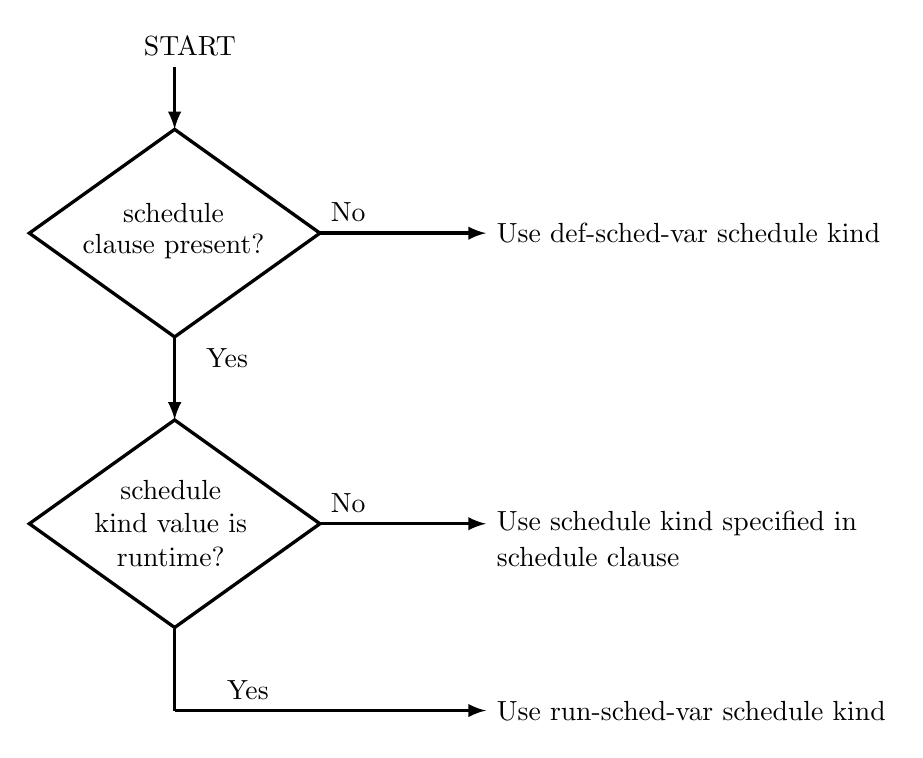
\begin{tikzpicture}
\pgftransformxscale{1.000000}
\pgftransformyscale{-1.000000}
\definecolor{dialinecolor}{rgb}{0.000000, 0.000000, 0.000000}
\pgfsetstrokecolor{dialinecolor}
\definecolor{dialinecolor}{rgb}{1.000000, 1.000000, 1.000000}
\pgfsetfillcolor{dialinecolor}
\definecolor{dialinecolor}{rgb}{1.000000, 1.000000, 1.000000}
\pgfsetfillcolor{dialinecolor}
\fill (18.500000\du,7.000000\du)--(22.000000\du,9.500000\du)--(18.500000\du,12.000000\du)--(15.000000\du,9.500000\du)--cycle;
\pgfsetlinewidth{0.080000\du}
\pgfsetdash{}{0pt}
\pgfsetdash{}{0pt}
\pgfsetmiterjoin
\definecolor{dialinecolor}{rgb}{0.000000, 0.000000, 0.000000}
\pgfsetstrokecolor{dialinecolor}
\draw (18.500000\du,7.000000\du)--(22.000000\du,9.500000\du)--(18.500000\du,12.000000\du)--(15.000000\du,9.500000\du)--cycle;
% setfont left to latex
\definecolor{dialinecolor}{rgb}{0.000000, 0.000000, 0.000000}
\pgfsetstrokecolor{dialinecolor}
\node at (18.500000\du,9.695000\du){};
\pgfsetlinewidth{0.080000\du}
\pgfsetdash{}{0pt}
\pgfsetdash{}{0pt}
\pgfsetbuttcap
{
\definecolor{dialinecolor}{rgb}{0.000000, 0.000000, 0.000000}
\pgfsetfillcolor{dialinecolor}
% was here!!!
\pgfsetarrowsend{latex}
\definecolor{dialinecolor}{rgb}{0.000000, 0.000000, 0.000000}
\pgfsetstrokecolor{dialinecolor}
\draw (18.500000\du,12.000000\du)--(18.500000\du,14.000000\du);
}
\pgfsetlinewidth{0.080000\du}
\pgfsetdash{}{0pt}
\pgfsetdash{}{0pt}
\pgfsetbuttcap
{
\definecolor{dialinecolor}{rgb}{0.000000, 0.000000, 0.000000}
\pgfsetfillcolor{dialinecolor}
% was here!!!
\pgfsetarrowsend{latex}
\definecolor{dialinecolor}{rgb}{0.000000, 0.000000, 0.000000}
\pgfsetstrokecolor{dialinecolor}
\draw (22.000000\du,16.500000\du)--(26.000000\du,16.500000\du);
}
% setfont left to latex
\definecolor{dialinecolor}{rgb}{0.000000, 0.000000, 0.000000}
\pgfsetstrokecolor{dialinecolor}
\node[anchor=west] at (20.000000\du,10.000000\du){};
\pgfsetlinewidth{0.080000\du}
\pgfsetdash{}{0pt}
\pgfsetdash{}{0pt}
\pgfsetbuttcap
{
\definecolor{dialinecolor}{rgb}{0.000000, 0.000000, 0.000000}
\pgfsetfillcolor{dialinecolor}
% was here!!!
\pgfsetarrowsend{latex}
\definecolor{dialinecolor}{rgb}{0.000000, 0.000000, 0.000000}
\pgfsetstrokecolor{dialinecolor}
\draw (18.500000\du,5.500000\du)--(18.500000\du,7.000000\du);
}
% setfont left to latex
\definecolor{dialinecolor}{rgb}{0.000000, 0.000000, 0.000000}
\pgfsetstrokecolor{dialinecolor}
\node[anchor=west] at (31.000000\du,12.000000\du){};
\definecolor{dialinecolor}{rgb}{1.000000, 1.000000, 1.000000}
\pgfsetfillcolor{dialinecolor}
\fill (18.500000\du,14.000000\du)--(22.000000\du,16.500000\du)--(18.500000\du,19.000000\du)--(15.000000\du,16.500000\du)--cycle;
\pgfsetlinewidth{0.080000\du}
\pgfsetdash{}{0pt}
\pgfsetdash{}{0pt}
\pgfsetmiterjoin
\definecolor{dialinecolor}{rgb}{0.000000, 0.000000, 0.000000}
\pgfsetstrokecolor{dialinecolor}
\draw (18.500000\du,14.000000\du)--(22.000000\du,16.500000\du)--(18.500000\du,19.000000\du)--(15.000000\du,16.500000\du)--cycle;
% setfont left to latex
\definecolor{dialinecolor}{rgb}{0.000000, 0.000000, 0.000000}
\pgfsetstrokecolor{dialinecolor}
\node at (18.500000\du,16.695000\du){};
\pgfsetlinewidth{0.080000\du}
\pgfsetdash{}{0pt}
\pgfsetdash{}{0pt}
\pgfsetbuttcap
{
\definecolor{dialinecolor}{rgb}{0.000000, 0.000000, 0.000000}
\pgfsetfillcolor{dialinecolor}
% was here!!!
\pgfsetarrowsend{latex}
\definecolor{dialinecolor}{rgb}{0.000000, 0.000000, 0.000000}
\pgfsetstrokecolor{dialinecolor}
\draw (22.000000\du,9.500000\du)--(26.000000\du,9.500000\du);
}
\pgfsetlinewidth{0.080000\du}
\pgfsetdash{}{0pt}
\pgfsetdash{}{0pt}
\pgfsetbuttcap
{
\definecolor{dialinecolor}{rgb}{0.000000, 0.000000, 0.000000}
\pgfsetfillcolor{dialinecolor}
% was here!!!
\definecolor{dialinecolor}{rgb}{0.000000, 0.000000, 0.000000}
\pgfsetstrokecolor{dialinecolor}
\draw (18.500000\du,19.040000\du)--(18.500000\du,21.000000\du);
}
\pgfsetlinewidth{0.080000\du}
\pgfsetdash{}{0pt}
\pgfsetdash{}{0pt}
\pgfsetbuttcap
{
\definecolor{dialinecolor}{rgb}{0.000000, 0.000000, 0.000000}
\pgfsetfillcolor{dialinecolor}
% was here!!!
\pgfsetarrowsend{latex}
\definecolor{dialinecolor}{rgb}{0.000000, 0.000000, 0.000000}
\pgfsetstrokecolor{dialinecolor}
\draw (18.500000\du,21.000000\du)--(26.000000\du,21.000000\du);
}
% setfont left to latex
\definecolor{dialinecolor}{rgb}{0.000000, 0.000000, 0.000000}
\pgfsetstrokecolor{dialinecolor}
\node[anchor=west] at (17.500000\du,5.000000\du){START};
% setfont left to latex
\definecolor{dialinecolor}{rgb}{0.000000, 0.000000, 0.000000}
\pgfsetstrokecolor{dialinecolor}
\node at (18.471967\du,9.021967\du){\code{schedule} 
};
% setfont left to latex
\definecolor{dialinecolor}{rgb}{0.000000, 0.000000, 0.000000}
\pgfsetstrokecolor{dialinecolor}
\node at (18.471967\du,9.821967\du){clause present?};
% setfont left to latex
\definecolor{dialinecolor}{rgb}{0.000000, 0.000000, 0.000000}
\pgfsetstrokecolor{dialinecolor}
\node at (18.408579\du,15.687353\du){schedule};
% setfont left to latex
\definecolor{dialinecolor}{rgb}{0.000000, 0.000000, 0.000000}
\pgfsetstrokecolor{dialinecolor}
\node at (18.408579\du,16.487353\du){kind value is};
% setfont left to latex
\definecolor{dialinecolor}{rgb}{0.000000, 0.000000, 0.000000}
\pgfsetstrokecolor{dialinecolor}
\node at (18.408579\du,17.287353\du){\code{runtime}?};
% setfont left to latex
\definecolor{dialinecolor}{rgb}{0.000000, 0.000000, 0.000000}
\pgfsetstrokecolor{dialinecolor}
\node[anchor=west] at (26.000000\du,9.500000\du){Use \plc{def-sched-var} schedule kind};
% setfont left to latex
\definecolor{dialinecolor}{rgb}{0.000000, 0.000000, 0.000000}
\pgfsetstrokecolor{dialinecolor}
\node[anchor=west] at (26.000000\du,16.500000\du){Use schedule kind specified in 
};
% setfont left to latex
\definecolor{dialinecolor}{rgb}{0.000000, 0.000000, 0.000000}
\pgfsetstrokecolor{dialinecolor}
\node[anchor=west] at (26.000000\du,17.300000\du){\code{schedule} clause};
% setfont left to latex
\definecolor{dialinecolor}{rgb}{0.000000, 0.000000, 0.000000}
\pgfsetstrokecolor{dialinecolor}
\node[anchor=west] at (26.000000\du,21.000000\du){Use \plc{run-sched-var} schedule kind};
% setfont left to latex
\definecolor{dialinecolor}{rgb}{0.000000, 0.000000, 0.000000}
\pgfsetstrokecolor{dialinecolor}
\node[anchor=west] at (22.000000\du,9.000000\du){No};
% setfont left to latex
\definecolor{dialinecolor}{rgb}{0.000000, 0.000000, 0.000000}
\pgfsetstrokecolor{dialinecolor}
\node[anchor=west] at (19.000000\du,12.500000\du){Yes};
% setfont left to latex
\definecolor{dialinecolor}{rgb}{0.000000, 0.000000, 0.000000}
\pgfsetstrokecolor{dialinecolor}
\node[anchor=west] at (22.000000\du,16.000000\du){No};
% setfont left to latex
\definecolor{dialinecolor}{rgb}{0.000000, 0.000000, 0.000000}
\pgfsetstrokecolor{dialinecolor}
\node[anchor=west] at (19.500000\du,20.500000\du){Yes};
\end{tikzpicture}

\end{quote}
\caption{Determining the \code{schedule} for a Worksharing Loop\label{fig:schedule loop}}
\end{figure}











\subsection{\code{sections} Construct}
\label{subsec:sections Construct}
\index{sections@{\code{sections}}}
\index{constructs!sections@{\code{sections}}}
\summary
The \code{sections} construct is a non-iterative worksharing construct that contains a set of 
structured blocks that are to be distributed among and executed by the threads in a team. 
Each structured block is executed once by one of the threads in the team in the context 
of its implicit task.

\syntax
\ccppspecificstart
The syntax of the \code{sections} construct is as follows:

\begin{boxedcode}
\#pragma omp sections \plc{[clause[ [},\plc{] clause] ... ] new-line}
   \{
   \plc{[}\#pragma omp section \plc{new-line}\plc{]}
      \plc{structured-block}
   \plc{[}\#pragma omp section \plc{new-line}
      \plc{structured-block]}
   \plc{...}
   \}
\end{boxedcode}

where \plc{clause} is one of the following: 

\begin{indentedcodelist}
private(\plc{list})
firstprivate(\plc{list})
lastprivate(\plc{list})
reduction(\plc{reduction-identifier }:\plc{ list})
nowait
\end{indentedcodelist}
\ccppspecificend

\needspace{16\baselineskip}\begin{samepage}
\fortranspecificstart
The syntax of the \code{sections} construct is as follows:

\begin{boxedcode}
!\$omp sections \plc{[clause[ [},\plc{] clause] ... ]}
   \plc{[}!\$omp section\plc{]}
      \plc{structured-block}
   \plc{[}!\$omp section
      \plc{structured-block]}
   \plc{...}
!\$omp end sections \plc{[}nowait\plc{]}
\end{boxedcode}
\end{samepage}

\begin{samepage}
where \plc{clause} is one of the following:

\begin{indentedcodelist}
private(\plc{list})
firstprivate(\plc{list})
lastprivate(\plc{list})
reduction(\plc{reduction-identifier }:\plc{ list})
\end{indentedcodelist}
\fortranspecificend
\end{samepage}

\binding
The binding thread set for a \code{sections} region is the current team. A \code{sections} 
region binds to the innermost enclosing \code{parallel} region. Only the threads of the team 
executing the binding \code{parallel} region participate in the execution of the structured 
blocks and the implied barrier of the \code{sections} region if the barrier is not eliminated 
by a \code{nowait} clause.

\descr
Each structured block in the \code{sections} construct is preceded by a \code{section} directive 
except possibly the first block, for which a preceding \code{section} directive is optional.

The method of scheduling the structured blocks among the threads in the team is 
implementation defined.

There is an implicit barrier at the end of a \code{sections} construct unless a \code{nowait} 
clause is specified.

\restrictions
Restrictions to the \code{sections} construct are as follows:

\begin{itemize}
\item Orphaned \code{section} directives are prohibited. That is, the \code{section} directives must 
appear within the \code{sections} construct and must not be encountered elsewhere in the 
\code{sections} region.

\item The code enclosed in a \code{sections} construct must be a structured block. 

\item Only a single \code{nowait} clause can appear on a \code{sections} directive.

\cppspecificstart
\item A throw executed inside a \code{sections} region must cause execution to resume within 
the same section of the \code{sections} region, and the same thread that threw the 
exception must catch it.
\cppspecificend
\end{itemize}

\crossreferences
\begin{itemize}
\item \code{private}, \code{firstprivate}, \code{lastprivate}, and \code{reduction} clauses, see 
\specref{subsec:Data-Sharing Attribute Clauses}.
\end{itemize}










\subsection{\code{single} Construct}
\index{single@{\code{single}}}
\index{constructs!single@{\code{single}}}
\label{subsec:single Construct}
\summary
The \code{single} construct specifies that the associated structured block is executed by only 
one of the threads in the team (not necessarily the master thread), in the context of its 
implicit task. The other threads in the team, which do not execute the block, wait at an 
implicit barrier at the end of the \code{single} construct unless a \code{nowait} clause is specified.

\parbox{\linewidth}{%
\syntax
\ccppspecificstart}
The syntax of the single construct is as follows:

\begin{boxedcode}
\#pragma omp single \plc{[clause[ [},\plc{] clause] ... ] new-line}
   \plc{structured-block}
\end{boxedcode}

\begin{samepage}
where \plc{clause} is one of the following:

\begin{indentedcodelist}
private(\plc{list})
firstprivate(\plc{list})
copyprivate(\plc{list})
nowait
\end{indentedcodelist}
\ccppspecificend
\end{samepage}

\fortranspecificstart
The syntax of the \code{single} construct is as follows:

\begin{boxedcode}
!\$omp single \plc{[clause[ [},\plc{] clause] ... ]}
   \plc{structured-block} 
!\$omp end single \plc{[end\_clause[ [},\plc{] end\_clause] ... ]}
\end{boxedcode}

where \plc{clause} is one of the following:

\begin{indentedcodelist}
private(\plc{list})
firstprivate(\plc{list})
\end{indentedcodelist}

and \plc{end\_clause} is one of the following: 

\begin{indentedcodelist}
copyprivate(\plc{list})
nowait
\end{indentedcodelist}
\fortranspecificend

\binding
The binding thread set for a \code{single} region is the current team. A \code{single} region 
binds to the innermost enclosing \code{parallel} region. Only the threads of the team 
executing the binding \code{parallel} region participate in the execution of the structured 
block and the implied barrier of the \code{single} region if the barrier is not eliminated by a 
\code{nowait} clause.

\descr
The method of choosing a thread to execute the structured block is implementation 
defined. There is an implicit barrier at the end of the \code{single} construct unless a 
\code{nowait} clause is specified. 

\restrictions
Restrictions to the \code{single} construct are as follows: 

\begin{itemize}
\item The \code{copyprivate} clause must not be used with the \code{nowait} clause.

\item At most one \code{nowait} clause can appear on a \code{single} construct.

\cppspecificstart
\item A throw executed inside a \code{single} region must cause execution to resume within the 
same \code{single} region, and the same thread that threw the exception must catch it.
\cppspecificend
\end{itemize}


\crossreferences
\begin{itemize}
\item \code{private} and \code{firstprivate} clauses, see 
\specref{subsec:Data-Sharing Attribute Clauses}.

\item \code{copyprivate} clause, see 
\specref{subsubsec:copyprivate clause}.
\end{itemize}













% Here we need to force the blue marker lower, and force the subsection header higher
% in order to reduce the space between the marker and the header, per Richard:
\begin{samepage}
\vspace{3\baselineskip}
\fortranspecificstart
\vspace{-3\baselineskip}
\subsection{\code{workshare} Construct}
\index{workshare@{\code{workshare}}}
\index{constructs!workshare@{\code{workshare}}}
\label{subsec:workshare Construct}
\summary
The \code{workshare} construct divides the execution of the enclosed structured block into 
separate units of work, and causes the threads of the team to share the work such that 
each unit is executed only once by one thread, in the context of its implicit task.
\end{samepage}

\begin{samepage}
\syntax
The syntax of the \code{workshare} construct is as follows:

\begin{boxedcode}
!\$omp workshare
    \plc{structured-block} 
!\$omp end workshare \plc{[}nowait\plc{]}
\end{boxedcode}
\end{samepage}

The enclosed structured block must consist of only the following:

\begin{itemize}
\item array assignments 

\item scalar assignments 

\item \code{FORALL} statements

\item \code{FORALL} constructs 

\item \code{WHERE} statements

\item \code{WHERE} constructs

\item \code{atomic} constructs

\item \code{critical} constructs

\item \code{parallel} constructs
\end{itemize}

Statements contained in any enclosed \code{critical} construct are also subject to these 
restrictions. Statements in any enclosed \code{parallel} construct are not restricted.

\binding
The binding thread set for a \code{workshare} region is the current team. A \code{workshare} 
region binds to the innermost enclosing \code{parallel} region. Only the threads of the team 
executing the binding \code{parallel} region participate in the execution of the units of 
work and the implied barrier of the \code{workshare} region if the barrier is not eliminated 
by a \code{nowait} clause.
% blue line floater at top of this page for "Fortran, cont."
\begin{figure}[t!]
\linewitharrows{-1}{dashed}{Fortran (cont.)}{8em}
\end{figure}

\descr
There is an implicit barrier at the end of a \code{workshare} construct unless a \code{nowait} 
clause is specified.

An implementation of the \code{workshare} construct must insert any synchronization that is 
required to maintain standard Fortran semantics. For example, the effects of one 
statement within the structured block must appear to occur before the execution of 
succeeding statements, and the evaluation of the right hand side of an assignment must 
appear to complete prior to the effects of assigning to the left hand side.

The statements in the \code{workshare} construct are divided into units of work as follows:

\begin{itemize}
\item For array expressions within each statement, including transformational array 
intrinsic functions that compute scalar values from arrays:

\begin{itemize} % nested level
\item Evaluation of each element of the array expression, including any references to 
\code{ELEMENTAL} functions, is a unit of work.

\item Evaluation of transformational array intrinsic functions may be freely subdivided 
into any number of units of work.
\end{itemize}

\item For an array assignment statement, the assignment of each element is a unit of work.

\item For a scalar assignment statement, the assignment operation is a unit of work.

\item For a \code{WHERE} statement or construct, the evaluation of the mask expression and the 
masked assignments are each a unit of work.

\item For a \code{FORALL} statement or construct, the evaluation of the mask expression, 
expressions occurring in the specification of the iteration space, and the masked 
assignments are each a unit of work

\item For an \code{atomic} construct, the atomic operation on the storage location designated as 
\plc{x} is a unit of work.

\item For a \code{critical} construct, the construct is a single unit of work.

\item For a \code{parallel} construct, the construct is a unit of work with respect to the 
\code{workshare} construct. The statements contained in the \code{parallel} construct are 
executed by a new thread team.

\item If none of the rules above apply to a portion of a statement in the structured block, 
then that portion is a unit of work.
\end{itemize}

The transformational array intrinsic functions are \code{MATMUL}, \code{DOT\_PRODUCT}, \code{SUM}, 
\code{PRODUCT}, \code{MAXVAL}, \code{MINVAL}, \code{COUNT}, 
\code{ANY}, \code{ALL}, \code{SPREAD}, \code{PACK}, \code{UNPACK}, 
\code{RESHAPE}, \code{TRANSPOSE}, \code{EOSHIFT}, \code{CSHIFT}, \code{MINLOC}, and \code{MAXLOC}.

It is unspecified how the units of work are assigned to the threads executing a 
\code{workshare} region.

If an array expression in the block references the value, association status, or allocation 
status of private variables, the value of the expression is undefined, unless the same 
value would be computed by every thread.

If an array assignment, a scalar assignment, a masked array assignment, or a \code{FORALL} 
assignment assigns to a private variable in the block, the result is unspecified.

The \code{workshare} directive causes the sharing of work to occur only in the \code{workshare} 
construct, and not in the remainder of the \code{workshare} region.

\begin{samepage}
\restrictions
The following restrictions apply to the \code{workshare} construct:

\begin{itemize}
\item All array assignments, scalar assignments, and masked array assignments must be 
intrinsic assignments.

\item The construct must not contain any user defined function calls unless the function is 
\code{ELEMENTAL}.
\end{itemize}
\fortranspecificend
\end{samepage}













\filbreak
\section{SIMD Constructs}
\label{sec:SIMD Constructs}
\index{SIMD Constructs}
\subsection{\code{simd} Construct}
\index{simd@{\code{simd}}}
\index{constructs!simd@{\code{simd}}}
\label{subsec:simd Construct}
\summary
The \code{simd} construct can be applied to a loop to indicate that the loop can be transformed 
into a SIMD loop (that is, multiple iterations of the loop can be executed concurrently 
using SIMD instructions).

\syntax
The syntax of the \code{simd} construct is as follows:

\ccppspecificstart
\begin{boxedcode}
\#pragma omp simd \plc{[clause[ [},\plc{] clause] ... ] new-line}
   \plc{for-loops}
\end{boxedcode}

where \plc{clause} is one of the following:

\begin{indentedcodelist}
safelen(\plc{length})
simdlen(\plc{length})
linear(\plc{list[ }:\plc{ linear-step]})
aligned(\plc{list[ }:\plc{ alignment]})
private(\plc{list})
lastprivate(\plc{list})
reduction(\plc{reduction-identifier }:\plc{ list})
collapse(\plc{n})
\end{indentedcodelist}

The \code{simd} directive places restrictions on the structure of the associated \plc{for-loops}. 
Specifically, all associated \plc{for-loops} must have \plc{canonical loop form} 
(\specref{sec:Canonical Loop Form}).
\ccppspecificend

\fortranspecificstart
\begin{boxedcode}
!\$omp simd \plc{[clause[ [},\plc{] clause ... ]}
   \plc{do-loops}
\plc{[}!\$omp end simd\plc{]}
\end{boxedcode}

where \plc{clause} is one of the following:

\begin{indentedcodelist}
safelen(\plc{length})
simdlen(\plc{length})
linear(\plc{list[ }:\plc{ linear-step]})
aligned(\plc{list[ }:\plc{ alignment]})
private(\plc{list})
lastprivate(\plc{list})
reduction(\plc{reduction-identifier }:\plc{ list})
collapse(\plc{n})
\end{indentedcodelist}

If an \code{end}~\code{simd} directive is not specified, an \code{end}~\code{simd} directive is assumed at the end 
of the \plc{do-loops}.

Any associated \plc{do-loop} must be a \plc{do-construct} or an 
\plc{inner-shared-do-construct} as defined by the Fortran standard. If an 
\code{end}~\code{simd} directive follows a \plc{do-construct} in which 
several loop statements share a \code{DO} termination statement, then the 
directive can only be specified for the outermost of these 
\code{DO} statements. 
\fortranspecificend

\binding
A \code{simd} region binds to the current task region. The binding thread set of the \code{simd} 
region is the current team.

\descr
The \code{simd} construct enables the execution of multiple iterations of the associated loops 
concurrently by means of SIMD instructions.

The \code{collapse} clause may be used to specify how many loops are associated with the 
construct. The parameter of the \code{collapse} clause must be a constant positive integer 
expression. If no \code{collapse} clause is present, the only loop that is associated with the 
loop construct is the one that immediately follows the directive.

If more than one loop is associated with the \code{simd} construct, then the iterations of all 
associated loops are collapsed into one larger iteration space that is then executed with 
SIMD instructions. The sequential execution of the iterations in all associated loops 
determines the order of the iterations in the collapsed iteration space.

The iteration count for each associated loop is computed before entry to the outermost 
loop. If execution of any associated loop changes any of the values used to compute any 
of the iteration counts, then the behavior is unspecified.

The integer type (or kind, for Fortran) used to compute the iteration count for the 
collapsed loop is implementation defined.

A SIMD loop has logical iterations numbered 0,1,...,N-1 where N is the number of loop 
iterations, and the logical numbering denotes the sequence in which the iterations would 
be executed if the associated loop(s) were executed with no SIMD instructions. If the 
\code{safelen} clause is used then no two iterations executed concurrently with SIMD 
instructions can have a greater distance in the logical iteration space than its value. The 
parameter of the \code{safelen} clause must be a constant positive integer expression. 
If used, the \code{simdlen} clause specifies the preferred number of iterations to be executed concurrently. 
The parameter of the \code{simdlen} clause must be a constant positive integer.
The number of iterations that are executed concurrently at any given time is implementation 
defined. Each concurrent iteration will be executed by a different SIMD lane. Each set 
of concurrent iterations is a SIMD chunk. Lexical forward dependencies in the iterations of the original loop must be preserved within each SIMD chunk.

\ccppspecificstart
The \code{aligned} clause declares that the object to which each list item points is aligned to 
the number of bytes expressed in the optional parameter of the \code{aligned} clause.
\ccppspecificend

\fortranspecificstart

The \code{aligned} clause declares that the location of each list item
is aligned to the number of bytes expressed in the optional parameter
of the \code{aligned} clause.

\fortranspecificend

The optional parameter of the \code{aligned} clause, \plc{alignment}, must be a constant positive 
integer expression. If no optional parameter is specified, implementation-defined default 
alignments for SIMD instructions on the target platforms are assumed.

\restrictions
\begin{itemize}
\item All loops associated with the construct must be perfectly nested; that is, there must be 
no intervening code nor any OpenMP directive between any two loops.

\item The associated loops must be structured blocks.

\item A program that branches into or out of a \code{simd} region is non-conforming. 

\item Only one \code{collapse} clause can appear on a \code{simd} directive.

\item A \plc{list-item} cannot appear in more than one \code{aligned} clause.

\item Only one \code{safelen} clause can appear on a \code{simd} directive.

\item Only one \code{simdlen} clause can appear on a \code{simd} directive.

\item If both \code{simdlen} and \code{safelen} clauses are specified, the value of the \code{simdlen} parameter must be less than or equal to the value of the \code{safelen} parameter.

\item A \plc{modifier} may not be specified on a \code{linear} clause.

\item An \code{ordered} construct with the \code{simd} clause is the only OpenMP
construct that can be encountered during execution of a \code{simd}
region.

\ccppspecificstart
\item The \code{simd} region cannot contain calls to the \code{longjmp} or \code{setjmp} functions. 
\ccppspecificend
\bigskip

\cspecificstart
\item The type of list items appearing in the \code{aligned} clause must be array or pointer.
\cspecificend

\cppspecificstart
\item The type of list items appearing in the \code{aligned} clause must be array, pointer, 
reference to array, or reference to pointer. 

\item No exception can be raised in the \code{simd} region. 
\cppspecificend

\fortranspecificstart
\item The \plc{do-loop} iteration variable must be of type \code{integer}.

\item The \plc{do-loop} cannot be a \code{DO WHILE} or a \code{DO} loop without loop control. 

\item If a list item on the \code{aligned} clause has the
  \code{ALLOCATABLE} attribute, the allocation status must be
  allocated.

\item If a list item on the \code{aligned} clause has the
  \code{POINTER} attribute, the association status must be associated.

\item If the type of a list item on the \code{aligned} clause is
  either \code{C\_PTR} or Cray pointer, the list item must be defined.

\fortranspecificend
\end{itemize}

\crossreferences
\begin{itemize}
\item \code{private}, \code{lastprivate}, \code{linear} and \code{reduction} clauses, see 
\specref{subsec:Data-Sharing Attribute Clauses}.
\end{itemize}








\subsection{\code{declare}~\code{simd} Construct}
\index{declare simd@{\code{declare}~\code{simd}}}
\index{constructs!declare simd@{\code{declare}~\code{simd}}}
\label{subsec:declare simd Construct}
\summary
The \code{declare}~\code{simd} construct can be applied to a function (C, C++ and Fortran) or a 
subroutine (Fortran) to enable the creation of one or more versions that can process 
multiple arguments using SIMD instructions from a single invocation in a SIMD 
loop. The \code{declare}~\code{simd} directive is a declarative directive. There may be multiple 
\code{declare}~\code{simd} directives for a function (C, C++, Fortran) or subroutine (Fortran).

\syntax
The syntax of the \code{declare}~\code{simd} construct is as follows:

\ccppspecificstart
\begin{boxedcode}
\#pragma omp declare simd \plc{[clause[ [},\plc{] clause] ... ] new-line}
\plc{[}\#pragma omp declare simd \plc{[clause[ [},\plc{] clause] ... ] new-line]}
\plc{[ ... ]}
   \plc{function definition or declaration}
\end{boxedcode}

where \plc{clause} is one of the following:

\begin{indentedcodelist}
simdlen(\plc{length})
linear(\plc{linear-list[ }:\plc{ linear-step]})
aligned(\plc{argument-list[ }:\plc{ alignment]})
uniform(\plc{argument-list})
inbranch
notinbranch
\end{indentedcodelist}
\ccppspecificend


\fortranspecificstart
\begin{boxedcode}
!\$omp declare simd \plc{[}(\plc{proc-name})\plc{] [clause[ [},\plc{] clause] ... ]}
\end{boxedcode}

where \plc{clause} is one of the following:
\begin{indentedcodelist}
simdlen(\plc{length})
linear(\plc{linear-list[ }:\plc{ linear-step]})
aligned(\plc{argument-list[ }:\plc{ alignment]})
uniform(\plc{argument-list})
inbranch
notinbranch
\end{indentedcodelist}
\fortranspecificend


\descr
\ccppspecificstart
The use of a \code{declare}~\code{simd} construct on a function enables the creation of SIMD 
versions of the associated function that can be used to process multiple arguments from 
a single invocation in a SIMD loop concurrently.

The expressions appearing in the clauses of this directive are evaluated in the scope of 
the arguments of the function declaration or definition.
\ccppspecificend

\begin{samepage}
\fortranspecificstart
The use of a \code{declare}~\code{simd} construct enables the creation of SIMD versions of the 
specified subroutine or function that can be used to process multiple arguments from a 
single invocation in a SIMD loop concurrently. 
\fortranspecificend
\end{samepage}

If a \code{declare}~\code{simd} directive contains multiple SIMD declarations,
each declaration enables the creation of SIMD versions.

If a SIMD version is created, the number of concurrent arguments for the function is 
determined by the \code{simdlen} clause. If the \code{simdlen} clause is used its value 
corresponds to the number of concurrent arguments of the function. The parameter of 
the \code{simdlen} clause must be a constant positive integer expression. Otherwise, the 
number of concurrent arguments for the function is implementation defined.

\cppspecificstart
The special \plc{this} pointer can be used as if was one of the arguments to the function in any of the \code{linear}, \code{aligned}, or \code{uniform} clauses.
\cppspecificend

The \code{uniform} clause declares one or more arguments to have an invariant value for all 
concurrent invocations of the function in the execution of a single SIMD loop.

\begin{samepage}
\ccppspecificstart
The \code{aligned} clause declares that the object to which each list item points is aligned to 
the number of bytes expressed in the optional parameter of the \code{aligned} clause.
\ccppspecificend
\end{samepage}

\needspace{15\baselineskip}\begin{samepage}
\fortranspecificstart
The \code{aligned} clause declares that the target of each list item is aligned to the number 
of bytes expressed in the optional parameter of the \code{aligned} clause.
\fortranspecificend
\end{samepage}

The optional parameter of the \code{aligned} clause, \plc{alignment}, must be a constant positive 
integer expression. If no optional parameter is specified, implementation-defined default 
alignments for SIMD instructions on the target platforms are assumed.

The \code{inbranch} clause specifies that the SIMD version of the function will always be called from inside a 
conditional statement of a SIMD loop. The \code{notinbranch} clause specifies that the 
SIMD version of the function will never be called from inside a conditional statement of a SIMD loop. If 
neither clause is specified, then the SIMD version of the function may or may not be called from inside a 
conditional statement of a SIMD loop.

\restrictions
\begin{itemize}
\item Each argument can appear in at most one \code{uniform} or \code{linear} clause.

\item At most one \code{simdlen} clause can appear in a \code{declare}~\code{simd} directive.

\item Either \code{inbranch} or \code{notinbranch} may be specified, but not both.

\item When a \plc{linear-step} expression is specified in a \code{linear} clause it must be
either a constant integer expression or an integer-typed parameter that is specified in
a \code{uniform} clause on the directive.

\item The function or subroutine body must be a structured block.

\item The execution of the function or subroutine, when called from a SIMD loop, cannot result in the execution of an OpenMP construct except for an \code{ordered} construct with the \code{simd} clause. 

\item The execution of the function or subroutine cannot have any side effects that would 
alter its execution for concurrent iterations of a SIMD chunk.

\item A program that branches into or out of the function is non-conforming.

\ccppspecificstart
\item If the function has any declarations, then the \code{declare}~\code{simd} construct for any 
declaration that has one must be equivalent to the one specified for the definition. 
Otherwise, the result is unspecified.

\item The function cannot contain calls to the \code{longjmp} or \code{setjmp} functions. 
\ccppspecificend

\cspecificstart
\item The type of list items appearing in the \code{aligned} clause must be array or pointer. 
\cspecificend

\cppspecificstart
\item The function cannot contain any calls to \code{throw}. 

\item The type of list items appearing in the \code{aligned} clause must be array, pointer, 
reference to array, or reference to pointer.
\cppspecificend

\fortranspecificstart
\item \plc{proc-name} must not be a generic name, procedure pointer or entry name.

\item If \plc{proc-name} is omitted, the \code{declare}~\code{simd}
  directive must appear in the specification part of a subroutine
  subprogram or a function subprogram for which creation of the SIMD
  versions is enabled.

\item Any \code{declare}~\code{simd} directive must appear in the specification part of a subroutine 
subprogram, function subprogram or interface body to which it applies.

\item If a \code{declare}~\code{simd} directive is specified in an interface block for a procedure, it 
must match a \code{declare}~\code{simd} directive in the definition of the procedure.

\item If a procedure is declared via a procedure declaration statement, the procedure 
\plc{proc-name} should appear in the same specification. 

\item If a \code{declare}~\code{simd} directive is specified for a procedure name with explicit 
interface and a \code{declare}~\code{simd} directive is also specified for the definition of the 
procedure then the two \code{declare}~\code{simd} directives must match. Otherwise the result 
is unspecified.

\item Procedure pointers may not be used to access versions created by the \code{declare}~\code{simd} directive.

\item The type of list items appearing in the \code{aligned} clause must be \code{C\_PTR} or Cray 
pointer, or the list item must have the \code{POINTER} or \code{ALLOCATABLE} attribute.
\fortranspecificend
\end{itemize}

\crossreferences
\begin{itemize}
\item \code{reduction} clause, see 
\specref{subsubsec:reduction clause}.

\item \code{linear} clause, see 
\specref{subsubsec:linear clause}.
\end{itemize}










\begin{samepage}
\subsection{Loop SIMD Construct}
\label{subsec:Loop SIMD Construct}
\index{loop SIMD Construct}
\index{constructs!Loop SIMD}
\index{do SIMD@{\code{do}~\code{simd}}}
\index{for SIMD@{\code{for}~\code{simd}}}
\summary
The loop SIMD construct specifies that the iterations of one or more associated loops will be distributed across threads that already exist in the team and that the iterations executed by each thread can also be executed concurrently using SIMD instructions. The loop SIMD construct is a composite construct.
\end{samepage}

\begin{samepage}
\syntax
\ccppspecificstart
\begin{boxedcode}
\#pragma omp for simd \plc{[clause[ [},\plc{] clause] ... ] new-line}
   \plc{for-loops}
\end{boxedcode}
\end{samepage}

where \plc{clause} can be any of the clauses accepted by the \code{for} or \code{simd} directives with 
identical meanings and restrictions.
\ccppspecificend

\fortranspecificstart
\begin{boxedcode}
!\$omp do simd \plc{[clause[ [},\plc{] clause] ... ]}
   \plc{do-loops}
\plc{[}!\$omp end do simd \plc{[}nowait\plc{] ]}
\end{boxedcode}

where \plc{clause} can be any of the clauses accepted by the \code{simd} or \code{do} directives, with 
identical meanings and restrictions.

If an \code{end}~\code{do}~\code{simd} directive is not specified, an \code{end}~\code{do}~\code{simd} directive is 
assumed at the end of the \plc{do-loops}.
\fortranspecificend

\descr
The loop SIMD construct will first distribute the iterations of the associated loop(s) 
across the implicit tasks of the parallel region in a manner consistent with any clauses 
that apply to the loop construct. The resulting chunks of iterations will then be converted 
to a SIMD loop in a manner consistent with any clauses that apply to the \code{simd} 
construct. The effect of any clause that applies to both constructs is as if it were applied to both constructs separately except the \code{collapse} clause, which is applied once.

\restrictions
All restrictions to the loop construct and the \code{simd} construct apply to the loop SIMD 
construct. In addition, the following restrictions apply:

\begin{itemize}
\item No \code{ordered} clause with a parameter can be specified.
\item A list item may appear in a \code{linear} or \code{firstprivate} clause but not both.
\end{itemize}

\begin{samepage}
\crossreferences
\begin{itemize}
\item loop construct, see 
\specref{subsec:Loop Construct}.

\item \code{simd} construct, see 
\specref{subsec:simd Construct}.

\item Data attribute clauses, see 
\specref{subsec:Data-Sharing Attribute Clauses}. 
\end{itemize}
\end{samepage}



\pagebreak
\section{Tasking Constructs}
\label{sec:Tasking Constructs}
\index{tasking constructs}
\index{constructs!tasking constructs}
\subsection{\code{task} Construct}
\index{task@{\code{task}}}
\index{constructs!task@{\code{task}}}
\label{subsec:task Construct}
\summary
The \code{task} construct defines an explicit task.

\begin{samepage}
\syntax
\ccppspecificstart
The syntax of the \code{task} construct is as follows: 

\begin{boxedcode}
\#pragma omp task \plc{[clause[ [},\plc{] clause] ... ] new-line}
    \plc{structured-block}
\end{boxedcode}
\end{samepage}

\begin{samepage}
where \plc{clause} is one of the following: 

\begin{indentedcodelist}
if(\plc{[} task :\plc{] scalar-expression})
final(\plc{scalar-expression})
untied
default(shared \textnormal{|} none)
mergeable
private(\plc{list})
firstprivate(\plc{list})
shared(\plc{list})
depend(\plc{dependence-type }:\plc{ list})
priority(\plc{priority-value})
\end{indentedcodelist}
\ccppspecificend
\end{samepage}

\fortranspecificstart
The syntax of the \code{task} construct is as follows: 

\begin{boxedcode}
!\$omp task \plc{[clause[ [},\plc{] clause] ... ]}
    \plc{structured-block}
!\$omp end task
\end{boxedcode}

where \plc{clause} is one of the following:

\begin{indentedcodelist}
if(\plc{[} task :\plc{] scalar-logical-expression})
final(\plc{scalar-logical-expression})
untied
default(private \textnormal{|} firstprivate \textnormal{|} shared \textnormal{|} none)
mergeable
private(\plc{list})
firstprivate(\plc{list})
shared(\plc{list})
depend(\plc{dependence-type }:\plc{ list})
priority(\plc{priority-value})
\end{indentedcodelist}
\fortranspecificend

\binding
The binding thread set of the \code{task} region is the current team. A \code{task} region binds to 
the innermost enclosing \code{parallel} region. 

\descr
When a thread encounters a \code{task} construct, a task is generated from the code for the 
associated structured block. The data environment of the task is created according to the 
data-sharing attribute clauses on the \code{task} construct, per-data environment ICVs, and 
any defaults that apply.

The encountering thread may immediately execute the task, or defer its execution. In the 
latter case, any thread in the team may be assigned the task. Completion of the task can 
be guaranteed using task synchronization constructs. 
If a \code{task} construct is encountered during execution of an outer
task, the generated \code{task} region associated with this construct is not a
part of the outer task region unless the generated task is
an included task.

When an \code{if} clause is present on a \code{task} construct, and the \code{if} clause expression 
evaluates to \plc{false}, an undeferred task is generated, and the encountering thread must 
suspend the current task region, for which execution cannot be resumed until the 
generated task is completed. The use of a variable in an \code{if} clause expression 
of a \code{task} construct causes an implicit reference to the variable in all enclosing 
constructs.

When a \code{final} clause is present on a \code{task} construct and the \code{final} clause expression 
evaluates to \plc{true}, the generated task will be a final task. All \code{task} constructs 
encountered during execution of a final task will generate final and included tasks. Note 
that the use of a variable in a \code{final} clause expression of a \code{task} construct causes an 
implicit reference to the variable in all enclosing constructs.

The \code{if} clause expression and the \code{final} clause expression are evaluated in the context 
outside of the \code{task} construct, and no ordering of those evaluations is specified.

A thread that encounters a task scheduling point within the \code{task} region may 
temporarily suspend the \code{task} region. By default, a task is tied and its suspended \code{task} 
region can only be resumed by the thread that started its execution. If the \code{untied} 
clause is present on a \code{task} construct, any thread in the team can resume the \code{task} 
region after a suspension. The \code{untied} clause is ignored if a \code{final} clause is present 
on the same \code{task} construct and the \code{final} clause expression evaluates to \plc{true}, or if a 
task is an included task.

The \code{task} construct includes a task scheduling point in the task region of its generating 
task, immediately following the generation of the explicit task. Each explicit \code{task} 
region includes a task scheduling point at its point of completion. 

When the \code{mergeable} clause is present on a \code{task} construct, the generated task is a \plc{mergeable task}. 

The \code{priority} clause is a hint for the priority of the generated task. The \plc{priority-value} is a
non-negative numerical scalar expression that provides a hint for task execution order. Among all
tasks ready to be executed, higher priority tasks (those with a higher numerical value in the
\code{priority} clause expression) are recommended to execute before lower priority ones. The default
\plc{priority-value} when no \code{priority} clause is specified is zero (the lowest priority). If a value is
specified in the \code{priority} clause that is higher than the \plc{max-task-priority-var} ICV then the
implementation will use the value of that ICV. A program that relies on task execution order
being determined by this \plc{priority-value} may have unspecified behavior.

\notestart
\noteheader – When storage is shared by an explicit \code{task} region, the 
programmer must ensure, by adding proper synchronization, that the storage does not 
reach the end of its lifetime before the explicit \code{task} region completes its execution.
\noteend

\restrictions
Restrictions to the \code{task} construct are as follows:

\begin{itemize}
\item A program that branches into or out of a \code{task} region is non-conforming. 

\item A program must not depend on any ordering of the evaluations of the clauses of the 
\code{task} directive, or on any side effects of the evaluations of the clauses. 

\item At most one \code{if} clause can appear on the directive. 

\item At most one \code{final} clause can appear on the directive.

\item At most one \code{priority} clause can appear on the directive.

\ccppspecificstart
\item A throw executed inside a \code{task} region must cause execution to resume within the 
same \code{task} region, and the same thread that threw the exception must catch it.
\ccppspecificend

\fortranspecificstart
\item Unsynchronized use of Fortran I/O statements by multiple tasks on the same unit has 
unspecified behavior
\fortranspecificend
\end{itemize}

\crossreferences
\begin{itemize}
\item Task scheduling constraints, see \specref{subsec:Task Scheduling}. 
\item \code{depend} clause, see \specref{subsec:depend Clause}.
\item \code{if} Clause, see \specref{sec:if Clause}.
\end{itemize}











% TASKLOOP 
\subsection{\code{taskloop} Construct}
\index{taskloop@{\code{taskloop}}}
\index{constructs!taskloop@{\code{taskloop}}}
\label{subsec:taskloop Construct}
\summary
The \code{taskloop} construct specifies that the iterations of one or more associated loops will be executed in parallel using OpenMP tasks. The iterations are distributed across tasks created by the construct and scheduled to be executed.
\syntax
\ccppspecificstart
The syntax of the \code{taskloop} construct is as follows:
\begin{boxedcode}
\#pragma omp taskloop \plc{[clause[[,] clause] ...] new-line}
    \plc{for-loops}
\end{boxedcode}
where \plc{clause} is one of the following:
\begin{indentedcodelist}
if(\plc{[} taskloop :\plc{] scalar-expr})
shared(\plc{list})
private(\plc{list})
firstprivate(\plc{list})
lastprivate(\plc{list})
default(shared \textnormal{|} none)
grainsize(\plc{grain-size})
num_tasks(\plc{num-tasks})
collapse(\plc{n})
final(\plc{scalar-expr})
priority(\plc{priority-value})
untied
mergeable
nogroup
\end{indentedcodelist}

The \code{taskloop} directive places restrictions on the structure of all associated \plc{for-loops}. Specifically, all associated \plc{for-loops} must have canonical loop form (see \specref{sec:Canonical Loop Form}).
\ccppspecificend
\fortranspecificstart
The syntax of the \code{taskloop} construct is as follows:
\begin{boxedcode}
!\$omp taskloop \plc{[clause[[,] clause] ...]}
    \plc{do-loops}
\plc{[}!\$omp end taskloop\plc{]}
\end{boxedcode}
where \plc{clause} is one of the following:
\begin{indentedcodelist}
if(\plc{[} taskloop :\plc{] scalar-logical-expr})
shared(\plc{list})
private(\plc{list})
firstprivate(\plc{list})
lastprivate(\plc{list})
default(private \textnormal{|} firstprivate \textnormal{|} shared \textnormal{|} none)
grainsize(\plc{grain-size})
num_tasks(\plc{num-tasks})
collapse(\plc{n})
final(\plc{scalar-logical-expr})
priority(\plc{priority-value})
untied
mergeable
nogroup
\end{indentedcodelist}

If an \code{end}~\code{taskloop} directive is not specified, an 
\code{end}~\code{taskloop} directive is assumed at the end of the 
\plc{do-loops}.

Any associated \plc{do-loop} must be \plc{do-construct} or an 
\plc{inner-shared-do-construct} as defined by the Fortran standard. 
If an \code{end}~\code{taskloop} directive follows a \plc{do-construct} 
in which several loop statements share a \code{DO} 
termination statement, then the directive can only be specified for the 
outermost of these \code{DO} statements.

If any of the loop iteration variables would otherwise be shared, they are implicitly made private for the loop-iteration tasks created by the \code{taskloop} construct. Unless the loop iteration variables are specified in a \code{lastprivate} clause on the \code{taskloop} construct, their values after the loop are unspecified.
\fortranspecificend

\binding
The binding thread set of the \code{taskloop} region is the current team. A \code{taskloop} region binds to the innermost enclosing \code{parallel} region.

\descr
When a thread encounters a \code{taskloop} construct, the construct partitions the associated loops into tasks for parallel execution of the loops' iterations. The data environment of the created tasks is created according to the data-sharing attribute clauses on the \code{taskloop} construct, per-data environment ICVs, and any defaults that apply. The order of the creation of the loop tasks is unspecified.
Programs that rely on any execution order of the logical loop iterations are non-conforming. 

If a \code{grainsize} clause is present on the \code{taskloop} construct, the number of logical loop iterations assigned to each created task is greater than or equal to the minimum of the value of the \plc{grain-size} expression and the number of logical loop iterations, but less than two times the value of the \plc{grain-size} expression.
The parameter of the \code{grainsize} clause must be a positive integer expression.
If \code{num\_tasks} is specified, the \code{taskloop} construct creates as many tasks as the minimum of the \plc{num-tasks} expression and the number of logical loop iterations.  
Each task must have at least one logical loop iteration.
The parameter of the \code{num\_tasks} clause must evaluate to a positive integer.
If neither a \code{grainsize} nor \code{num\_tasks} clause is present, the number of loop tasks created and the number of logical loop iterations assigned to these tasks is implementation defined.

The \code{collapse} clause may be used to specify how many loops are associated with the \code{taskloop} construct. The parameter of the \code{collapse} clause must be a constant positive integer expression. If no \code{collapse} clause is present, the only loop that is associated with the \code{taskloop} construct is the one that immediately follows the \code{taskloop} directive.

If more than one loop is associated with the \code{taskloop} construct, then the iterations of all associated loops are collapsed into one larger iteration space that is then divided according to the \code{grainsize} and \code{num\_tasks} clauses. The sequential execution of the iterations in all associated loops determines the order of the iterations in the collapsed iteration space. 
%% TODO: Does this conflict with the note about the independence of loop iterations below?

The iteration count for each associated loop is computed before entry to the outermost loop. If execution of any associated loop changes any of the values used to compute any of the iteration counts, then the behavior is unspecified. 

The integer type (or kind, for Fortran) used to compute the iteration count for the collapsed loop is implementation defined.

When an \code{if} clause is present on a \code{taskloop} construct, and if the \code{if} clause expression evaluates to \plc{false}, undeferred tasks are generated. The use of a variable in an \code{if} clause expression of a \code{taskloop} construct causes an implicit reference to the variable in all enclosing constructs.

When a \code{final} clause is present on a \code{taskloop} construct and the \code{final} clause expression evaluates to \plc{true}, the generated tasks will be final tasks. The use of a variable in a \code{final} clause expression of a \code{taskloop} construct causes an implicit reference to the variable in all enclosing constructs.

When a \code{priority} clause is present on a \code{taskloop} construct,
the generated tasks have the \plc{priority-value} as if it was 
specified for each individual task.  
If the \code{priority} clause is not specified, tasks generated by 
the \code{taskloop} construct have the default task priority (zero).

If the \code{untied} clause is specified, all tasks created by the \code{taskloop} construct are untied tasks.

When the \code{mergeable} clause is present on a \code{taskloop} construct, each generated task is a \plc{mergeable task}. 

By default, the \code{taskloop} construct executes as if it was enclosed in a \code{taskgroup} construct with no statements or directives outside of the \code{taskloop} construct. Thus, the \code{taskloop} construct creates an implicit \code{taskgroup} region. If the \code{nogroup} clause is present, no implicit \code{taskgroup} region is created.

\cppspecificstart
For \code{firstprivate} variables of class type, the number of invocations of copy constructors to perform the initialization  is implementation-defined.
\cppspecificend

\notestart
\noteheader – When storage is shared by a \code{taskloop} region, the programmer must ensure, by adding proper synchronization, that the storage does not reach the end of its lifetime before the \code{taskloop} region and its descendant tasks complete their execution.
\noteend

\restrictions
The restrictions of the \code{taskloop} construct are as follows:
\begin{itemize}
\item A program that branches into or out of a \code{taskloop} region is non-conforming.
\item All loops associated with the \code{taskloop} construct must be perfectly nested; that is, there must be no intervening code nor any OpenMP directive between any two loops.
\item At most one \code{grainsize} clause can appear on a \code{taskloop} directive.
\item At most one \code{num\_tasks} clause can appear on a \code{taskloop} directive.
\item The \code{grainsize} clause and \code{num\_tasks} clause are mutually exclusive and may not appear on the same \code{taskloop} directive.
\item At most one \code{collapse} clause can appear on a \code{taskloop} directive.
\item At most one \code{if} clause can appear on the directive.
\item At most one \code{final} clause can appear on the directive. 
\item At most one \code{priority} clause can appear on the directive.
\end{itemize}

\crossreferences
\begin{itemize}
\item \code{task} construct, \specref{subsec:task Construct}.
\item \code{taskgroup} construct, \specref{subsec:taskgroup Construct}.
\item Data-sharing attribute clauses, \specref{subsec:Data-Sharing Attribute Clauses}. 
\item \code{if} Clause, see \specref{sec:if Clause}.
\end{itemize}






%
%TASKLOOP SIMD
%
\subsection{\code{taskloop}~\code{simd} Construct}
\index{taskloop simd@{\code{taskloop}~\code{simd}}}
\index{constructs!taskloop simd@{\code{taskloop}~\code{simd}}}
\label{subsec:taskloop simd Construct}
\summary
The \code{taskloop}~\code{simd} construct specifies a loop that can be 
executed concurrently using SIMD instructions and that those iterations 
will also be executed in parallel using OpenMP tasks. The \code{taskloop}
\code{simd} construct is a composite construct.

\syntax
\ccppspecificstart
The syntax of the \code{taskloop}~\code{simd} construct is as follows:
\begin{boxedcode}
\#pragma omp taskloop simd \plc{[clause[[,] clause] ...] new-line}
    \plc{for-loops}
\end{boxedcode}
where \plc{clause} can be any of the clauses accepted by the \code{taskloop} or \code{simd} directives with identical meanings and restrictions.
\ccppspecificend
\fortranspecificstart
The syntax of the \code{taskloop}~\code{simd} construct is as follows:
\begin{boxedcode}
!\$omp taskloop simd \plc{[clause[[,] clause] ...]}
    \plc{do-loops}
\plc{[}!\$omp end taskloop simd\plc{]}
\end{boxedcode}
where \plc{clause} can be any of the clauses accepted by the \code{taskloop} or \code{simd} directives with identical meanings and restrictions.

If an \code{end}~\code{taskloop}~\code{simd} directive is not specified, an \code{end}~\code{taskloop}~\code{simd} directive is assumed at the end of the \plc{do-loops}.
\fortranspecificend

\binding
The binding thread set of the \code{taskloop}~\code{simd} region is the current team. A \code{taskloop}~\code{simd} region binds to the innermost enclosing parallel region.

\descr
The \code{taskloop}~\code{simd} construct will first distribute the iterations of the associated loop(s) across tasks in a manner consistent with any clauses that apply to the \code{taskloop} construct. The resulting tasks will then be converted to a SIMD loop in a manner consistent with any clauses that apply to the \code{simd} construct. The effect of any clause that applies to both constructs is as if it were applied to both constructs separately except the \code{collapse} clause, which is applied once.

\restrictions
\begin{itemize}
\item The restrictions for the \code{taskloop} and \code{simd} constructs apply.
\item No \code{reduction} clause can be specified. 
\end{itemize}

\crossreferences
\begin{itemize}
\item \code{taskloop} construct, see \specref{subsec:taskloop Construct}.
\item \code{simd} construct, see \specref{subsec:simd Construct}.
\item Data-sharing attribute clauses, see \specref{subsec:Data-Sharing Attribute Clauses}. 
\end{itemize}




%
%   TASKYIELD CONSTRUCT
%
\subsection{\code{taskyield} Construct}
\index{taskyield@{\code{taskyield}}}
\index{constructs!taskyield@{\code{taskyield}}}
\label{subsec:taskyield Construct}
\summary
The \code{taskyield} construct specifies that the current task can be suspended in favor of 
execution of a different task. The \code{taskyield} construct is a stand-alone directive.

\syntax
\ccppspecificstart
The syntax of the \code{taskyield} construct is as follows:

\begin{boxedcode}
\#pragma omp taskyield \plc{new-line}
\end{boxedcode}
\ccppspecificend

\fortranspecificstart
The syntax of the \code{taskyield} construct is as follows:

\begin{boxedcode}
!\$omp taskyield
\end{boxedcode}
\fortranspecificend

\binding
A \code{taskyield} region binds to the current task region. The binding thread set of the 
\code{taskyield} region is the current team.

\descr
The \code{taskyield} region includes an explicit task scheduling point in the current task 
region.

\crossreferences
\begin{itemize}
\item Task scheduling, see 
\specref{subsec:Task Scheduling}. 
\end{itemize}













\subsection{Task Scheduling}
\index{task scheduling}
\index{scheduling}
\label{subsec:Task Scheduling}
Whenever a thread reaches a task scheduling point, the implementation may cause it to 
perform a task switch, beginning or resuming execution of a different task bound to the 
current team. Task scheduling points are implied at the following locations:

\begin{itemize}
\item the point immediately following the generation of an explicit task;

\item after the point of completion of a \code{task} region;

\item in a \code{taskyield} region;

\item in a \code{taskwait} region;

\item at the end of a \code{taskgroup} region;

\item in an implicit and explicit \code{barrier} region;

\item the point immediately following the generation of a \code{target} region;

\item at the beginning and end of a \code{target}~\code{data} region;

\item in a \code{target}~\code{update} region; 

\item in a \code{target}~\code{enter}~\code{data} region; 

\item in a \code{target}~\code{exit}~\code{data} region; 

\item in the \code{omp\_target\_memcpy} routine; 

\item in the \code{omp\_target\_memcpy\_rect} routine;

\end{itemize}

When a thread encounters a task scheduling point it may do one of the following, 
subject to the \emph{Task Scheduling Constraints} (below):

\begin{itemize}
\item begin execution of a tied task bound to the current team

\item resume any suspended task region, bound to the current team, to which it is tied

\item begin execution of an untied task bound to the current team

\item resume any suspended untied task region bound to the current team.
\end{itemize}

If more than one of the above choices is available, it is unspecified as to which will be 
chosen.

\emph{Task Scheduling Constraints} are as follows:

\begin{enumerate}
\item An included task is executed immediately after generation of the task.

\item Scheduling of new tied tasks is constrained by the set of task regions that are currently 
tied to the thread, and that are not suspended in a \code{barrier} region. If this set is empty, 
any new tied task may be scheduled. Otherwise, a new tied task may be scheduled only 
if it is a descendent task of every task in the set.

\item A dependent task shall not be scheduled until its task dependences are fulfilled.

\item When an explicit task is generated by a construct containing an \code{if} clause for which the 
expression evaluated to \plc{false}, and the previous constraints are already met, the task is 
executed immediately after generation of the task.
\end{enumerate}

A program relying on any other assumption about task scheduling is non-conforming.

\notestart
\noteheader – Task scheduling points dynamically divide task regions into parts. Each part is 
executed uninterrupted from start to end. Different parts of the same task region are 
executed in the order in which they are encountered. In the absence of task 
synchronization constructs, the order in which a thread executes parts of different 
schedulable tasks is unspecified.

A correct program must behave correctly and consistently with all conceivable 
scheduling sequences that are compatible with the rules above.

For example, if \code{threadprivate} storage is accessed (explicitly in the source code or 
implicitly in calls to library routines) in one part of a task region, its value cannot be 
assumed to be preserved into the next part of the same task region if another schedulable 
task exists that modifies it.

As another example, if a lock acquire and release happen in different parts of a task 
region, no attempt should be made to acquire the same lock in any part of another task 
that the executing thread may schedule. Otherwise, a deadlock is possible. A similar 
situation can occur when a \code{critical} region spans multiple parts of a task and another 
schedulable task contains a \code{critical} region with the same name.

The use of threadprivate variables and the use of locks or critical sections in an explicit 
task with an \code{if} clause must take into account that when the \code{if} clause evaluates to 
\plc{false}, the task is executed immediately, without regard to \emph{Task Scheduling Constraint}~2.
\noteend





\section{Device Constructs}
\label{sec:Device Constructs}
\index{device constructs}
\index{constructs!device constructs}
\index{device constructs!device constructs}

\subsection{\code{target}~\code{data} Construct}
\index{target data@{\code{target}~\code{data}}}
\index{constructs!target data@{\code{target}~\code{data}}}
\label{subsec:target data Construct}
\summary
 Map variables to a device data environment for the extent of the region.
\syntax
\ccppspecificstart
The syntax of the \code{target}~\code{data} construct is as follows:

\begin{boxedcode}
\#pragma omp target data \plc{clause[ [ [},\plc{] clause] ... ] new-line}
    \plc{structured-block}
\end{boxedcode}

\needspace{10\baselineskip}\begin{samepage}
where \plc{clause} is one of the following:

\begin{indentedcodelist}
if(\plc{[} target data :\plc{] scalar-expression})
device(\plc{integer-expression})
map(\plc{[[map-type-modifier[,]] map-type}:\plc{ ] list})
use\_device\_ptr(\plc{list})
\end{indentedcodelist}
\ccppspecificend
\medskip
\end{samepage}

\fortranspecificstart
The syntax of the \code{target}~\code{data} construct is as follows:

\begin{boxedcode}
!\$omp target data \plc{clause[ [ [},\plc{] clause] ... ]}
    \plc{structured-block}
!\$omp end target data
\end{boxedcode}

where \plc{clause} is one of the following:

\begin{indentedcodelist}
if(\plc{[} target data :\plc{] scalar-logical-expression})
device(\plc{scalar-integer-expression})
map(\plc{[[map-type-modifier[,]] map-type}:\plc{ ] list})
use\_device\_ptr(\plc{list})
\end{indentedcodelist}

The \code{end}~\code{target}~\code{data} directive denotes the end of the \code{target}~\code{data} construct.
\fortranspecificend

\binding
The binding task set for a \code{target}~\code{data} region is the generating task. The 
\code{target}~\code{data} region binds to the region of the generating task.

\descr
When a \code{target}~\code{data} construct is encountered, the encountering task executes the region. If there is no \code{device} clause, the default device is determined by the \plc{default-device-var} ICV. Variables are mapped for the extent of the region, according to any data-mapping clauses, from the data environment of the encountering task to the device data environment. When an \code{if} clause is present and the \code{if} clause expression evaluates to \plc{false}, the device is the host.

List items that appear in a \code{use\_device\_ptr} clause are converted into
device pointers to the corresponding list item in the device data environment.

\restrictions
\begin{itemize}
  \item A program must not depend on any ordering of the evaluations of the clauses of the
    \code{target}~\code{data} directive, or on any side effects of the evaluations of the clauses.

  \item At most one \code{device} clause can appear on the directive. The \code{device} expression
    must evaluate to a non-negative integer value less than the value
    of \code{omp\_get\_num\_devices()}.

  \item At most one \code{if} clause can appear on the directive.
  \item A \plc{map-type} in a \code{map} clause must be \code{to}, \code{from}, \code{tofrom} or \code{alloc}.
  \item At least one \code{map} clause must appear on the directive.


  \item A list item in a \code{use\_device\_ptr} clause must have a
    corresponding list item in the device data environment.

  \item References in the construct to a list item that appears in a
    \code{use\_device\_ptr} clause must be to the address of the list item.
\end{itemize}

\crossreferences
\begin{itemize}
\item \plc{default-device-var}, see 
\specref{sec:Internal Control Variables}. 

\item \code{if} Clause, see \specref{sec:if Clause}.

\item \code{map} clause, see 
\specref{subsec:map Clause}.
\end{itemize}










\subsection{\code{target}~\code{enter}~\code{data} Construct}
\label{subsec:target enter data Construct}
\index{constructs!target enter data@{\code{target}~\code{enter}~\code{data}}}
\index{device data environments}
\summary
The \code{target}~\code{enter}~\code{data} directive specifies that variables are mapped to a device data environment. The \code{target}~\code{enter}~\code{data} directive is a stand-alone directive.
\syntax
\ccppspecificstart
The syntax of the \code{target}~\code{enter}~\code{data} construct is as follows:
\begin{boxedcode}
\#pragma omp target enter data \plc{[ clause[ [,] clause]...] new-line}
\end{boxedcode}
where \plc{clause} is one of the following:
\begin{indentedcodelist}
if(\plc{[} target enter data :\plc{] scalar-expression})
device(\plc{integer-expression})
map(\plc{[ [map-type-modifier[,]] map-type} : \plc{] list})
depend(\plc{dependence-type} : \plc{list})
nowait
\end{indentedcodelist}
\ccppspecificend
\fortranspecificstart
The syntax of the \code{target}~\code{enter}~\code{data} is as follows:
\begin{boxedcode}
!\$omp target enter data \plc{[ clause[ [,] clause]...]}
\end{boxedcode}
where clause is one of the following:
\begin{indentedcodelist}
if(\plc{[} target enter data :\plc{] scalar-logical-expression})
device(\plc{scalar-integer-expression})
map(\plc{[ [map-type-modifier[,]] map-type} : \plc{] list})
depend(\plc{dependence-type} : \plc{list})
nowait
\end{indentedcodelist}
\fortranspecificend

\binding
The binding task set for a \code{target}~\code{enter}~\code{data} region is
the generating task, which is the \plc{target task} generated by the
\code{target}~\code{enter}~\code{data} construct. The
\code{target}~\code{enter}~\code{data} region binds to the corresponding
\plc{target task} region.

\descr
When a \code{target}~\code{enter}~\code{data} construct is encountered, the list items are mapped to the device data environment according to the \code{map} clause semantics.

The \code{target}~\code{enter}~\code{data} construct is a task generating construct.  The generated task is a \plc{target task}.  The generated task region encloses the \code{target}~\code{enter}~\code{data} region.

All clauses are evaluated when the \code{target}~\code{enter}~\code{data} construct is encountered.  The data environment of the \plc{target task} is created according to the data-sharing attribute clauses on the \code{target}~\code{enter}~\code{data} construct, per-data environment ICVs, and any default data-sharing attribute rules that apply to the \code{target}~\code{enter}~\code{data} construct.  A variable that is mapped in the \code{target}~\code{enter}~\code{data} construct has a default data-sharing attribute of shared in the data environment of the \plc{target task}.

Assignment operations associated with mapping a variable ({see \specref{subsec:map Clause}) occur when the \plc{target task} executes.

If the \code{nowait} clause is present, execution of the \plc{target task} may be deferred.  If the \code{nowait} clause is not present, the \plc{target task} is an included task.

If a \code{depend} clause is present, it is associated with the \plc{target task}.

If there is no \code{device} clause, the default device is determined by the \plc{default-device-var} ICV.

When an \code{if} clause is present and the \code{if} clause expression evaluates to \plc{false}, the device is the host. 

\restrictions
\begin{itemize}
\item A program must not depend on any ordering of the evaluations of the clauses of the \code{target}~\code{enter}~\code{data} directive, or on any side effects of the evaluations of the clauses.
\item At least one \code{map} clause must appear on the directive.
\item At most one \code{device} clause can appear on the directive. The \code{device} expression must evaluate to a non-negative integer value.
\item At most one \code{if} clause can appear on the directive.
\item A \plc{map-type} must be specified in all \code{map} clauses and must be either \code{to} or \code{alloc}.
\end{itemize}

\crossreferences
\begin{itemize}
\item \plc{default-device-var}, see \specref{subsec:ICV Descriptions}.

\item \code{task}, see \specref{subsec:task Construct}.

\item \code{task}~\code{scheduling}~\code{constraints}, 
      see \specref{subsec:Task Scheduling}. 

\item \code{target}~\code{data}, see \specref{subsec:target data Construct}.

\item \code{target}~\code{exit}~\code{data}, 
      see \specref{subsec:target exit data Construct}.

\item \code{if} Clause, see \specref{sec:if Clause}.

\item \code{map} clause, see \specref{subsec:map Clause}.
\end{itemize}





\subsection{\code{target}~\code{exit}~\code{data} Construct}
\label{subsec:target exit data Construct}
\index{constructs!target exit data@{\code{target}~\code{exit}~\code{data}}}
\index{device data environments}
\summary
The \code{target}~\code{exit}~\code{data} directive specifies that list items are unmapped from a device data environment. The \code{target}~\code{exit}~\code{data} directive is a stand-alone directive.
\syntax
\ccppspecificstart
The syntax of the \code{target}~\code{exit}~\code{data} construct is as follows:
\begin{boxedcode}
\#pragma omp target exit data \plc{[ clause[ [,] clause]...] new-line}
\end{boxedcode}
where \plc{clause} is one of the following:
\begin{indentedcodelist}
if(\plc{[} target exit data :\plc{] scalar-expression})
device(\plc{integer-expression})
map(\plc{[ [map-type-modifier[,]] map-type} : \plc{] list})
depend(\plc{dependence-type} : \plc{list})
nowait
\end{indentedcodelist}
\ccppspecificend
\fortranspecificstart
The syntax of the \code{target}~\code{exit}~\code{data} is as follows:
\begin{boxedcode}
!\$omp target exit data \plc{[ clause[ [,] clause]...]}
\end{boxedcode}
where clause is one of the following:
\begin{indentedcodelist}
if(\plc{[} target exit data :\plc{] scalar-logical-expression})
device(\plc{scalar-integer-expression})
map(\plc{[ [map-type-modifier[,]] map-type} : \plc{] list})
depend(\plc{dependence-type} : \plc{list})
nowait
\end{indentedcodelist}
\fortranspecificend

\begin{samepage}

\binding
The binding task set for a \code{target}~\code{exit}~\code{data} region is
the generating task, which is the \plc{target task} generated by the
\code{target}~\code{exit}~\code{data} construct. The
\code{target}~\code{exit}~\code{data} region binds to the corresponding
\plc{target task} region.

\descr
When a \code{target}~\code{exit}~\code{data} construct is encountered, the list items in the \code{map} clauses are unmapped from the device data environment according to the \code{map} clause semantics.

The \code{target}~\code{exit}~\code{data} construct is a task generating construct.  The generated task is a \plc{target task}.  The generated task region encloses the \code{target}~\code{exit}~\code{data} region.

All clauses are evaluated when the \code{target}~\code{exit}~\code{data} construct is encountered.  The data environment of the \plc{target task} is created according to the data-sharing attribute clauses on the \code{target}~\code{exit}~\code{data} construct, per-data environment ICVs, and any default data-sharing attribute rules that apply to the \code{target}~\code{exit}~\code{data} construct.  A variable that is mapped in the \code{target}~\code{exit}~\code{data} construct has a default data-sharing attribute of shared in the data environment of the \plc{target task}.

\end{samepage}

Assignment operations associated with mapping a variable ({see \specref{subsec:map Clause}) occur when the \plc{target task} executes.

If the \code{nowait} clause is present, execution of the \plc{target task} may be deferred.  If the \code{nowait} clause is not present, the \plc{target task} is an included task.

If a \code{depend} clause is present, it is associated with the \plc{target task}.

If there is no \code{device} clause, the default device is determined by the \plc{default-device-var} ICV.

When an \code{if} clause is present and the \code{if} clause expression evaluates to \plc{false}, the device is the host. 
\restrictions
\begin{itemize}
\item A program must not depend on any ordering of the evaluations of the clauses of the \code{target}~\code{exit}~\code{data} directive, or on any side effects of the evaluations of the clauses.
\item At least one \code{map} clause must appear on the directive.
\item At most one \code{device} clause can appear on the directive. The \code{device} expression must evaluate to a non-negative integer value.
\item At most one \code{if} clause can appear on the directive.
\item A \plc{map-type} must be specified in all \code{map} clauses and must be either \code{from}, \code{release}, or \code{delete}.
\end{itemize}

\crossreferences
\begin{itemize}
\item \plc{default-device-var}, see \specref{subsec:ICV Descriptions}.

\item \code{task}, see \specref{subsec:task Construct}.

\item \code{task}~\code{scheduling}~\code{constraints}, 
      see \specref{subsec:Task Scheduling}. 

\item \code{target}~\code{data}, see \specref{subsec:target data Construct}.

\item \code{target}~\code{enter}~\code{data}, 
      see \specref{subsec:target enter data Construct}.

\item \code{if} Clause, see \specref{sec:if Clause}.

\item \code{map} clause, see \specref{subsec:map Clause}.
\end{itemize}





\pagebreak

\subsection{\code{target} Construct}
\index{target@{\code{target}}}
\index{constructs!target@{\code{target}}}
\index{device constructs!target@{\code{target}}}
\label{subsec:target Construct}
\summary
Map variables to a device data environment and execute the construct on that device.
\syntax
\ccppspecificstart
The syntax of the \code{target} construct is as follows:

\begin{boxedcode}
\#pragma omp target \plc{[clause[ [},\plc{] clause] ... ] new-line}
    \plc{structured-block}
\end{boxedcode}

where \plc{clause} is one of the following:

\begin{indentedcodelist}
if(\plc{[} target :\plc{] scalar-expression})
device(\plc{integer-expression})
private(\plc{list})
firstprivate(\plc{list})
map(\plc{[[map-type-modifier[,]] map-type}:\plc{ ] list})
is\_device\_ptr(\plc{list})
defaultmap(tofrom:scalar)
nowait
depend(\plc{dependence-type}: \plc{list})
\end{indentedcodelist}
\ccppspecificend

\begin{samepage}
\smallskip
\fortranspecificstart
The syntax of the \code{target} construct is as follows:

\begin{boxedcode}
!\$omp target \plc{[clause[ [},\plc{] clause] ... ]}
    \plc{structured-block}
!\$omp end target
\end{boxedcode}
\end{samepage}

\begin{samepage}
where \plc{clause} is one of the following:

\begin{indentedcodelist}
if(\plc{[} target :\plc{] scalar-logical-expression})
device(\plc{scalar-integer-expression})
private(\plc{list})
firstprivate(\plc{list})
map(\plc{[[map-type-modifier[,]] map-type}:\plc{ ] list})
is\_device\_ptr(\plc{list})
defaultmap(tofrom:scalar)
nowait
depend (\plc{dependence-type} : \plc{list})
\end{indentedcodelist}
\end{samepage}

The \code{end}~\code{target} directive denotes the end of the \code{target} construct
\fortranspecificend

\binding
The binding task set for a \code{target} region is the
generating task, which is the \plc{target task} generated
by the \code{target} construct. The \code{target}
region binds to the corresponding \plc{target task} region.

\descr
The \code{target} construct provides a superset of the functionality
provided by the \code{target}~\code{data} directive, except for 
the \code{use\_device\_ptr} clause.

The functionality added to the \code{target} directive is the inclusion of an executable region to be executed by a device. That is, the \code{target} directive is an executable directive.

The \code{target} construct is a task generating construct.  The generated task is a \plc{target task}.  The generated task region encloses the \code{target} region.

All clauses are evaluated when the \code{target} construct is encountered.  The data environment of the \plc{target task} is created according to the data-sharing attribute clauses on the \code{target} construct, per-data environment ICVs, and any default data-sharing attribute rules that apply to the \code{target} construct.  A variable that is mapped in the \code{target} construct has a default data-sharing attribute of shared in the data environment of the \plc{target task}.

Assignment operations associated with mapping a variable ({see \specref{subsec:map Clause}) occur when the \plc{target task} executes.

If the \code{nowait} clause is present, execution of the \plc{target task} may be deferred.  If the \code{nowait} clause is not present, the \plc{target task} is an included task.

If a \code{depend} clause is present, it is associated with the \plc{target task}.

When an \code{if} clause is present and the \code{if} clause expression evaluates to \plc{false}, the \code{target} region is executed by the host device in the host data environment.

The \code{is\_device\_ptr} clause is used to indicate that a list item is a device
pointer already in the device data environment and that it should be used
directly.  Support for device pointers created outside of OpenMP, specifically
outside of the \code{omp\_target\_alloc} routine and the \code{use\_device\_ptr} clause,
is implementation defined.

\ccppspecificstart
If an array section is a list item in a \code{map} clause and the array section is derived from a variable for which the type is pointer then the data-sharing attribute for that variable in the construct is firstprivate.  Prior to the execution of the construct, the private variable is initialized with the address of the storage location of the corresponding array section in the device data environment.

If a zero-length array section is a list item in a \code{map} clause, and the array section is derived from a variable for the which the type is pointer then that variable is initialized with the address of the corresponding storage location in the device data environment.  If the corresponding storage location is not present in the device data environment then the private variable is initialized to NULL.  
\ccppspecificend

\restrictions
\begin{itemize}
\item If a \code{target}, \code{target}~\code{update}, 
\code{target}~\code{data}, \code{target}~\code{enter}~\code{data}, or 
\code{target}~\code{exit}~\code{data} construct is encountered during
execution of a \code{target} region, the behavior is unspecified.

\item The result of an \code{omp\_set\_default\_device}, 
\code{omp\_get\_default\_device}, or \code{omp\_get\_num\_devices} 
routine called within a \code{target} region is unspecified.

\item The effect of an access to a \code{threadprivate} variable in a target region is 
unspecified.

\item If a list item in a \code{map} clause is a structure element, any other 
element of that structure that is referenced in the \code{target} construct 
must also appear as a list item in a \code{map} clause.

\item A variable referenced in a \code{target} region but not the \code{target} construct that is not 
declared in the \code{target} region must appear in a \code{declare}~\code{target} directive. 

\item At most one \code{defaultmap} clause can appear on the directive.

\item A \plc{map-type} in a \code{map} clause must be \code{to}, \code{from}, \code{tofrom} or \code{alloc}.

\item A list item that appears in an \code{is\_device\_ptr} clause must be a valid device pointer in the device data environment.

\cspecificstart
\item A list item that appears in an \code{is\_device\_ptr} clause must have a type of pointer or array.
\cspecificend

\cppspecificstart
\item A list item that appears in an \code{is\_device\_ptr} clause must have a type
  of pointer, array, reference to pointer or reference to array.
\item A throw executed inside a \code{target} region must cause execution to resume within the
same \code{target} region, and the same thread that threw the exception must catch it. 
\cppspecificend

\fortranspecificstart
\item A list item that appears in an \code{is\_device\_ptr} clause must be a dummy
  argument.
\item If a list item in a \code{map} clause is an array section, and the array section is derived from a variable with a \code{POINTER} or \code{ALLOCATABLE} attribute then the behavior is unspecified if the corresponding list item's variable is modified in the region.
\fortranspecificend
\end{itemize}

\crossreferences
\begin{itemize}
\item \plc{default-device-var}, see 
\specref{sec:Internal Control Variables}. 

\item \code{task} construct, see 
\specref{subsec:task Construct}.

\item \code{task} scheduling constraints, see 
\specref{subsec:Task Scheduling}

\item \code{target}~\code{data} construct, see 
\specref{subsec:target data Construct}.

\item \code{if} Clause, see \specref{sec:if Clause}.

\item \code{private} and \code{firstprivate} clauses, see 
\specref{subsec:Data-Sharing Attribute Clauses}.

\item Data-mapping Attribute Rules and Clauses, see 
\specref{subsec:Data-mapping Attribute Rules and Clauses}.
\end{itemize}







\vspace{-24pt}

\subsection{\code{target}~\code{update} Construct}
\index{target update@{\code{target}~\code{update}}}
\index{constructs!target update@{\code{target}~\code{update}}}
\index{device constructs!target update@{\code{target}~\code{update}}}
\label{subsec:target update Construct}
\summary
The \code{target}~\code{update} directive makes the corresponding list items in the device data 
environment consistent with their original list items, according to the specified motion 
clauses. The \code{target}~\code{update} construct is a stand-alone directive.

\syntax
\ccppspecificstart
The syntax of the \code{target}~\code{update} construct is as follows:

\begin{boxedcode}
\#pragma omp target update \plc{clause[ [ [},\plc{] clause] ... ] new-line}
\end{boxedcode}
where \plc{clause} is either \plc{motion-clause} or one of the following:

\begin{indentedcodelist}
if(\plc{[} target update :\plc{] scalar-expression})
device(\plc{integer-expression})
nowait
depend (\plc{dependence-type} : \plc{list})
\end{indentedcodelist}

and \plc{motion-clause} is one of the following:

\begin{indentedcodelist}
to(\plc{list})
from(\plc{list})
\end{indentedcodelist}
\ccppspecificend

\fortranspecificstart
The syntax of the \code{target}~\code{update} construct is as follows:

\begin{boxedcode}
!\$omp target update \plc{clause[ [ [},\plc{] clause] ... ]}
\end{boxedcode}

where \plc{clause} is either \plc{motion-clause} or one of the following:

\begin{indentedcodelist}
if(\plc{[}target update :\plc{] scalar-logical-expression})
device(\plc{scalar-integer-expression})
nowait
depend (\plc{dependence-type} : \plc{list})
\end{indentedcodelist}

and \plc{motion-clause} is one of the following:

\begin{indentedcodelist}
to(\plc{list})
from(\plc{list})
\end{indentedcodelist}
\fortranspecificend

\begin{samepage}

\binding
The binding task set for a \code{target}~\code{update} region is the
generating task, which is the \plc{target task} generated
by the \code{target}~\code{update} construct. The \code{target}~\code{update}
region binds to the corresponding \plc{target task} region.

\descr
For each list item in a \code{to} or \code{from} clause there is a corresponding list item and an 
original list item. If the corresponding list item is not present in the device data environment then no assignment occurs to or from the original list item. Otherwise, each corresponding list item in the 
device data environment has an original list item in the current task's data environment.

For each list item in a \code{from} clause the value of the corresponding list item is assigned 
to the original list item.

For each list item in a \code{to} clause the value of the original list item is assigned to the 
corresponding list item.

\end{samepage}

The list items that appear in the \code{to} or \code{from} clauses may include array sections.

The \code{target}~\code{update} construct is a task generating construct.  The generated task is a \plc{target task}.  The generated task region encloses the \code{target}~\code{update} region.

All clauses are evaluated when the \code{target}~\code{update} construct is encountered.  The data environment of the \plc{target task} is created according to the data-sharing attribute clauses on the \code{target}~\code{update} construct, per-data environment ICVs, and any default data-sharing attribute rules that apply to the \code{target}~\code{update} construct.  A variable that is mapped in the \code{target}~\code{update} construct has a default data-sharing attribute of shared in the data environment of the \plc{target task}.

Assignment operations associated with mapping a variable ({see \specref{subsec:map Clause}) occur when the \plc{target task} executes.

If the \code{nowait} clause is present, execution of the \plc{target task} may be deferred.  If the \code{nowait} clause is not present, the \plc{target task} is an included task.

If a \code{depend} clause is present, it is associated with the \plc{target task}.

The device is specified in the \code{device} clause. If there is no \code{device} clause, the device 
is determined by the \plc{default-device-var} ICV. When an \code{if} clause is present and the \code{if} 
clause expression evaluates to \plc{false} then no assignments occur.

\restrictions
\begin{itemize}
\item A program must not depend on any ordering of the evaluations of the clauses of the 
\code{target}~\code{update} directive, or on any side effects of the evaluations of the clauses. 

\item At least one \plc{motion-clause} must be specified.

\item If a list item is an array section it must specify contiguous storage. 

\item A list item can only appear in a \code{to} or \code{from} clause, but not both.

\item A list item in a \code{to} or \code{from} clause must have a mappable type.

\item At most one \code{device} clause can appear on the directive. The \code{device} expression
      must evaluate to a non-negative integer value less than the value
      of \code{omp\_get\_num\_devices()}.

\item At most one \code{if} clause can appear on the directive. 
\end{itemize}

\crossreferences
\begin{itemize}
\item \plc{default-device-var}, see 
\specref{sec:Internal Control Variables}.

\item Array sections, 
\specref{sec:Array Sections}

\item \code{task} construct, see 
\specref{subsec:task Construct}.

\item \code{task} scheduling constraints, see 
\specref{subsec:Task Scheduling}

\item \code{target}~\code{data}, see 
\specref{subsec:target data Construct}. 

\item \code{if} Clause, see \specref{sec:if Clause}.


\end{itemize}










\subsection{\code{declare}~\code{target} Directive}
\index{declare target@{\code{declare}~\code{target}}}
\index{directives!declare target@{\code{declare}~\code{target}}}
\index{constructs!declare target@{\code{declare}~\code{target}}}
\index{device constructs!declare target@{\code{declare}~\code{target}}}
\label{subsec:declare target Directive}
\summary
The \code{declare}~\code{target} directive specifies that variables, 
functions (C, C++ and Fortran), and subroutines (Fortran) are mapped 
to a device. The \code{declare}~\code{target} directive is a declarative 
directive.

\syntax
\ccppspecificstart
The syntax of the \code{declare}~\code{target} directive takes either of 
the following forms:

\begin{boxedcode}
\#pragma omp declare target \plc{new-line}
\plc{declaration-definition-seq}
\#pragma omp end declare target \plc{new-line}
\end{boxedcode}

or

\begin{boxedcode}
\#pragma omp declare target (\plc{extended-list}) \plc{new-line}
\end{boxedcode}

or

\begin{boxedcode}
\#pragma omp declare target \plc{clause[ [},\plc{] clause ... ] new-line}
\end{boxedcode}

where \plc{clause} is one of the following:

\begin{indentedcodelist}
to(\plc{extended-list})
link(\plc{list})
\end{indentedcodelist}
\ccppspecificend

\begin{samepage}

\fortranspecificstart
The syntax of the \code{declare}~\code{target} directive is as follows:

\begin{boxedcode}
!\$omp declare target (\plc{extended-list})
\end{boxedcode}

or

\begin{boxedcode}
!\$omp declare target \plc{[clause[ [},\plc{] clause] ... ]} 
\end{boxedcode}

where \plc{clause} is one of the following:

\begin{indentedcodelist}
to(\plc{extended-list})
link(\plc{list})
\end{indentedcodelist}
\fortranspecificend

\descr

The \code{declare} \code{target} directive ensures that procedures
and global variables can be executed or accessed on a device.
Variables are mapped for all device executions, or for specific
device executions through a \code{link} clause.

If an \plc{extended-list} is present with no clause then the \code{to}
clause is assumed.

If a list item of a \code{to} clause is a function (C, C++, Fortran) 
or subroutine (Fortran) then a device-specific version of the routine is 
created that can be called from a \code{target} region.

\end{samepage}

If a list item of a \code{to} clause is a variable then the original 
variable is mapped to a corresponding variable in the device data environment 
of all devices as if it had appeared in a \code{map} clause with the
\plc{map-type} \code{to} on the implicit \code{target}~\code{data} construct 
for each device. The list item is never removed from those device data 
environments as if its reference count is initialized to positive infinity.

The list items of a \code{link} clause are not mapped 
by the \code{declare}~\code{target} directive. Instead, their mapping
is deferred until they are mapped by \code{target}~\code{data} 
or \code{target} constructs. They are mapped only for such regions.

\pagebreak
\ccppspecificstart
The form of the \code{declare}~\code{target} directive that has no clauses 
and requires a matching \code{end}~\code{declare}~\code{target} directive
defines an implicit \plc{extended-list} to an implicit \code{to}
clause. The implicit \plc{extended-list} consists of the variable names 
of any variable declarations at file or namespace scope that appear between 
the two directives and of the function names of any function declarations at 
file, namespace or class scope that appear between the two directives.
\ccppspecificend

\fortranspecificstart
If a \code{declare}~\code{target} does not have any clauses then an implicit 
\plc{extended-list} to an implicit \code{to} clause of one item is formed from
the name of the enclosing subroutine subprogram, function subprogram or 
interface body to which it applies.
\fortranspecificend

\restrictions
\begin{itemize}
\item A threadprivate variable cannot appear in a 
      \code{declare}~\code{target} directive.

\item A variable declared in a \code{declare}~\code{target} directive 
      must have a mappable type.

\item The same list item must not appear multiple times in clauses on the same directive.

\item The same list item must not appear in both a \code{to} clause on one
\code{declare}~\code{target} directive and a \code{link} clause on
another \code{declare}~\code{target} directive.

\ccppspecificstart
\item All declarations and definitions for a function must have a 
      \code{declare}~\code{target} directive if one is specified for 
      any of them. Otherwise, the result is unspecified.

\item The \plc{declaration-definition-seq} defined by a 
      \code{declare}~\code{target} directive and an 
      \code{end}~\code{declare}~\code{target} directive must not contain
      any \code{declare}~\code{target} directives.
\end{itemize}
\ccppspecificend

\cppspecificstart
\begin{itemize}
\item The function names of overloaded functions or template functions
may only be specified within an implicit \plc{extended-list}.
\end{itemize}
\cppspecificend

\fortranspecificstart
\begin{itemize}
\item If a list item is a procedure name, it must not be a generic name, 
      procedure pointer or entry name.

\item Any \code{declare}~\code{target} directive with clauses must appear 
      in a specification part of a subroutine subprogram, function subprogram,
      program or module.

\item Any \code{declare}~\code{target} directive without clauses must appear 
      in a specification part of a subroutine subprogram, function subprogram 
      or interface body to which it applies.

\item If a \code{declare}~\code{target} directive is specified in an 
      interface block for a procedure, it must match a 
      \code{declare}~\code{target} directive in the definition of the 
      procedure.

\item If an external procedure is a type-bound procedure of a derived 
      type and a \code{declare}~\code{target} directive is specified in 
      the definition of the external procedure, such a directive must 
      appear in the interface block that is accessible to the derived 
      type definition.

\item If any procedure is declared via a procedure declaration statement 
      that is not in the type-bound procedure part of a derived-type 
      definition, any \code{declare}~\code{target} with the procedure 
      name must appear in the same specification part.

\item A variable that is part of another variable (as an array or structure 
      element) cannot appear in a \code{declare}~\code{target} directive.

\item The \code{declare}~\code{target} directive must appear in the 
      declaration section of a scoping unit in which the common block 
      or variable is declared. Although variables in common blocks can 
      be accessed by use association or host association, common block 
      names cannot. This means that a common block name specified in a 
      \code{declare}~\code{target} directive must be declared to be a 
      common block in the same scoping unit in which the 
      \code{declare}~\code{target} directive appears.

\item If a \code{declare}~\code{target} directive specifying a common 
      block name appears in one program unit, then such a directive must 
      also appear in every other program unit that contains a \code{COMMON} 
      statement specifying the same name. It must appear after the last 
      such \code{COMMON} statement in the program unit.

\item If a list item is declared with the \code{BIND} attribute, the 
      corresponding C entities must also be specified in a 
      \code{declare}~\code{target} directive in the C program.

\item A blank common block cannot appear in a \code{declare}~\code{target} 
      directive.

\item A variable can only appear in a \code{declare}~\code{target} directive 
      in the scope in which it is declared. It must not be an element of a 
      common block or appear in an \code{EQUIVALENCE} statement.

\item A variable that appears in a \code{declare}~\code{target} directive 
      must be declared in the Fortran scope of a module or have the 
      \code{SAVE} attribute, either explicitly or implicitly. 
\end{itemize}
\fortranspecificend







\subsection{\code{teams} Construct}
\index{teams@{\code{teams}}}
\index{constructs!teams@{\code{teams}}}
\index{device constructs!teams@{\code{teams}}}
\label{subsec:teams Construct}
\summary
The \code{teams} construct creates a league of thread teams and the master thread of each 
team executes the region.

\syntax
\ccppspecificstart
The syntax of the \code{teams} construct is as follows:

\begin{boxedcode}
\#pragma omp teams \plc{[clause[ [},\plc{] clause] ... ] new-line}
    \plc{structured-block}
\end{boxedcode}

where \plc{clause} is one of the following:

\begin{indentedcodelist}
num\_teams(\plc{integer-expression})
thread\_limit(\plc{integer-expression})
default(shared \textnormal{|} none)
private(\plc{list})
firstprivate(\plc{list})
shared(\plc{list})
reduction(\plc{reduction-identifier }:\plc{ list})
\end{indentedcodelist}
\ccppspecificend

\fortranspecificstart
The syntax of the \code{teams} construct is as follows:

\begin{boxedcode}
!\$omp teams \plc{[clause[ [},\plc{] clause] ... ]}
    \plc{structured-block}
!\$omp end teams
\end{boxedcode}

where \plc{clause} is one of the following:

\begin{indentedcodelist}
num\_teams(\plc{scalar-integer-expression})
thread\_limit(\plc{scalar-integer-expression})
default(shared \textnormal{|} firstprivate \textnormal{|} private \textnormal{|} none)
private(\plc{list})
firstprivate(\plc{list})
shared(\plc{list})
reduction(\plc{reduction-identifier }:\plc{ list})
\end{indentedcodelist}

The \code{end}~\code{teams} directive denotes the end of the \code{teams} construct.
\fortranspecificend

\begin{samepage}

\binding
The binding thread set for a \code{teams} region is the encountering thread,
which is the initial thread of the \code{target} region.

\descr
When a thread encounters a \code{teams} construct, a league of thread teams is created and 
the master thread of each thread team executes the \code{teams} region.

The number of teams created is implementation defined, but is less than or equal to the 
value specified in the \code{num\_teams} clause.
A thread may obtain the number of teams by a call to the \code{omp\_get\_num\_teams} routine.

\end{samepage}

The maximum number of threads participating in the contention group that each team 
initiates is implementation defined, but is less than or equal to the value specified in the 
\code{thread\_limit} clause.

On a combined or composite construct that includes \code{target} and
\code{teams} constructs, the expressions in \code{num\_teams} and
\code{thread\_limit} clauses are evaluated on the host device on
entry to the \code{target} construct.

Once the teams are created, the number of teams remains constant for the duration of the 
\code{teams} region.

Within a \code{teams} region, team numbers uniquely identify each team. Team numbers are 
consecutive whole numbers ranging from zero to one less than the number of teams. A 
thread may obtain its own team number by a call to the \code{omp\_get\_team\_num} library 
routine.

After the teams have completed execution of the \code{teams} region, the encountering thread 
resumes execution of the enclosing \code{target} region.

There is no implicit barrier at the end of a \code{teams} construct.

\restrictions
Restrictions to the \code{teams} construct are as follows:

\begin{itemize}
\item A program that branches into or out of a \code{teams} region is non-conforming.

\item A program must not depend on any ordering of the evaluations of the clauses of the 
\code{teams} directive, or on any side effects of the evaluation of the clauses.

\item At most one \code{thread\_limit} clause can appear on the directive. The 
\code{thread\_limit} expression must evaluate to a positive integer value.

\item At most one \code{num\_teams} clause can appear on the directive. The \code{num\_teams}
expression must evaluate to a positive integer value.

\item If specified, a \code{teams} construct must be contained within a \code{target} construct. That \code{target} construct must contain no statements, declarations or directives outside of the \code{teams} construct.

\item \code{distribute}, \code{distribute simd}, distribute parallel loop,
distribute parallel loop SIMD, and \code{parallel} regions, including any
\code{parallel} regions arising from combined constructs, are the only OpenMP regions
that may be strictly nested inside the \code{teams} region.

\end{itemize}

\crossreferences
\begin{itemize}

\item \code{default}, \code{shared}, \code{private}, \code{firstprivate}, and \code{reduction} clauses, see 
\specref{subsec:Data-Sharing Attribute Clauses}.

\item \code{omp\_get\_num\_teams} routine, see 
\specref{subsec:omp_get_num_teams}.

\item \code{omp\_get\_team\_num} routine, see 
\specref{subsec:omp_get_team_num}.
\end{itemize}









\subsection{\code{distribute} Construct}
\index{distribute@{\code{distribute}}}
\index{constructs!distribute@{\code{distribute}}}
\index{device constructs!distribute@{\code{distribute}}}
\label{subsec:distribute Construct}
\summary
The \code{distribute} construct specifies that the iterations of one or more loops will be 
executed by the thread teams in the context of their implicit tasks. The iterations are 
distributed across the master threads of all teams that execute the \code{teams} region to 
which the \code{distribute} region binds.

\syntax
\ccppspecificstart
The syntax of the \code{distribute} construct is as follows:

\begin{boxedcode}
\#pragma omp distribute \plc{[clause[ [},\plc{] clause] ... ] new-line}
   \plc{for-loops}
\end{boxedcode}

Where \plc{clause} is one of the following:

\begin{indentedcodelist}
private(\plc{list})
firstprivate(\plc{list})
lastprivate(\plc{list})
collapse(\plc{n})
dist\_schedule(\plc{kind[},\plc{ chunk\_size]})
\end{indentedcodelist}

All associated \plc{for-loops} must have the canonical form described in 
\specref{sec:Canonical Loop Form}.
\ccppspecificend
\bigskip

\fortranspecificstart
The syntax of the \code{distribute} construct is as follows:

\begin{boxedcode}
!\$omp distribute \plc{[clause[ [},\plc{] clause] ... ]}
   \plc{do-loops}
\plc{[}!\$omp end distribute\plc{]}
\end{boxedcode}

Where \plc{clause} is one of the following:

\begin{indentedcodelist}
private(\plc{list})
firstprivate(\plc{list})
lastprivate(\plc{list})
collapse(\plc{n})
dist\_schedule(\plc{kind[},\plc{ chunk\_size]})
\end{indentedcodelist}

If an \code{end}~\code{distribute} directive is not specified, an \code{end}~\code{distribute} directive 
is assumed at the end of the \plc{do-loops}.

Any associated \plc{do-loop} must be a \plc{do-construct} or an
\plc{inner-shared-do-construct} as defined by the Fortran standard. If an 
\code{end}~\code{distribute} directive follows a \plc{do-construct} in which several loop statements share a \code{DO} 
termination statement, then the directive can only be specified for the outermost of these 
\code{DO} statements.
\fortranspecificend

\begin{samepage}

\binding
The binding thread set for a \code{distribute} region is the set of master
threads executing an enclosing \code{teams} region. A \code{distribute} region
binds to this \code{teams} region. Only the threads executing the binding \code{teams} region participate in the 
execution of the loop iterations.

\descr
The \code{distribute} construct is associated with a loop nest consisting of one or more 
loops that follow the directive.

There is no implicit barrier at the end of a \code{distribute} construct.
To avoid data races the original
list items modified due to \code{lastprivate} or \code{linear} clauses
should not be accessed between the end of the \code{distribute} construct and the end
of the \code{teams} region to which the \code{distribute} binds.

\end{samepage}

The \code{collapse} clause may be used to specify how many loops are associated with the 
\code{distribute} construct. The parameter of the \code{collapse} clause must be a constant 
positive integer expression. If no \code{collapse} clause is present, the only loop that is 
associated with the \code{distribute} construct is the one that immediately follows the 
\code{distribute} construct.

If more than one loop is associated with the \code{distribute} construct, then the iteration 
of all associated loops are collapsed into one larger iteration space. The sequential 
execution of the iterations in all associated loops determines the order of the iterations in 
the collapsed iteration space.

The iteration count for each associated loop is computed before entry to the outermost loop. If execution of any associated loop changes any of the values used to compute any of the iteration counts, then the behavior is unspecified. 

The integer type (or kind, for Fortran) used to compute the iteration count for the collapsed loop is implementation defined.

If \code{dist\_schedule} is specified, \plc{kind} must be \code{static}. If specified, iterations are 
divided into chunks of size \plc{chunk\_size}, chunks are assigned to the teams of the league in 
a round-robin fashion in the order of the team number. When no \plc{chunk\_size} is specified, 
the iteration space is divided into chunks that are approximately equal in size, and at 
most one chunk is distributed to each team of the league. The size of the 
chunks is unspecified in this case.

When no \code{dist\_schedule} clause is specified, the schedule is implementation defined.

\restrictions
Restrictions to the \code{distribute} construct are as follows:

\begin{itemize}
\item The \code{distribute} construct inherits the restrictions of the loop construct.

\item The region associated with the \code{distribute} construct must be
strictly nested inside a \code{teams} region.

\item A list item may appear in a \code{firstprivate} or \code{lastprivate} clause but not both.
\end{itemize}

\crossreferences
\begin{itemize}
\item loop construct, see 
\specref{subsec:Loop Construct}.

\item \code{teams} construct, see 
\specref{subsec:teams Construct}
\end{itemize}










\subsection{\code{distribute}~\code{simd} Construct}
\index{distribute simd@{\code{distribute}~\code{simd}}}
\index{constructs!distribute simd@{\code{distribute}~\code{simd}}}
\index{device constructs!distribute simd@{\code{distribute}~\code{simd}}}
\label{subsec:distribute simd Construct}
\summary
The \code{distribute}~\code{simd} construct specifies a loop that will be distributed across the 
master threads of the \code{teams} region and executed concurrently using SIMD instructions. The \code{distribute}~\code{simd} construct is a composite construct.

\syntax
The syntax of the \code{distribute}~\code{simd} construct is as follows:

\ccppspecificstart
\begin{boxedcode}
\#pragma omp distribute simd \plc{[clause[ [},\plc{] clause] ... ] newline}
   \plc{for-loops}
\end{boxedcode}

where \plc{clause} can be any of the clauses accepted by the \code{distribute} or \code{simd} 
directives with identical meanings and restrictions.
\ccppspecificend

\fortranspecificstart
\begin{boxedcode}
!\$omp distribute simd \plc{[clause[ [},\plc{] clause] ... ]}
   \plc{do-loops}
\plc{[}!\$omp end distribute simd\plc{]}
\end{boxedcode}

where \plc{clause} can be any of the clauses accepted by the \code{distribute} or \code{simd} 
directives with identical meanings and restrictions.

If an \code{end}~\code{distribute}~\code{simd} directive is not specified, an \code{end}~\code{distribute}~\code{simd}
directive is assumed at the end of the \plc{do-loops}.
\fortranspecificend

\descr
The \code{distribute}~\code{simd} construct will first distribute the iterations of the associated 
loop(s) according to the semantics of the \code{distribute} construct and any clauses that 
apply to the distribute construct. The resulting chunks of iterations will then be 
converted to a SIMD loop in a manner consistent with any clauses that apply to the 
\code{simd} construct. The effect of any clause that applies to both constructs is as if it were applied to both constructs separately except the \code{collapse} clause, which is applied once.

\restrictions
\begin{itemize}
\item The restrictions for the \code{distribute} and \code{simd} constructs apply.

\item A list item may not appear in a \code{linear} clause, unless it is the loop iteration variable.
\end{itemize}

\crossreferences
\begin{itemize}
\item \code{simd} construct, see 
\specref{subsec:simd Construct}.

\item \code{distribute} construct, see 
\specref{subsec:distribute Construct}.

\item Data attribute clauses, see 
\specref{subsec:Data-Sharing Attribute Clauses}.
\end{itemize}









\subsection{Distribute Parallel Loop Construct}
\index{distribute parallel loop construct}
\index{constructs!distribute parallel loop}
\index{device constructs!distribute parallel loop}
\index{constructs!distribute parallel for@{\code{distribute}~\code{parallel}~\code{for}}}
\index{constructs!distribute parallel do@{\code{distribute}~\code{parallel}~\code{do}}}
\label{subsec:Distribute Parallel Loop Construct}
\summary
The distribute parallel loop construct specifies a loop that can be executed in parallel by 
multiple threads that are members of multiple teams. The distribute parallel loop construct is a composite construct.

\syntax
The syntax of the distribute parallel loop construct is as follows:

\ccppspecificstart
\begin{boxedcode}
\#pragma omp distribute parallel for \plc{[clause[ [},\plc{] clause] ... ] newline}
    \plc{for-loops}
\end{boxedcode}

where \plc{clause} can be any of the clauses accepted by the \code{distribute} or parallel loop 
directives with identical meanings and restrictions.
\ccppspecificend

\fortranspecificstart
\begin{boxedcode}
!\$omp distribute parallel do \plc{[clause[ [},\plc{] clause] ... ]}
    \plc{do-loops}
\plc{[}!\$omp end distribute parallel do\plc{]}
\end{boxedcode}

where \plc{clause} can be any of the clauses accepted by the \code{distribute} or parallel loop 
directives with identical meanings and restrictions.

If an \code{end}~\code{distribute}~\code{parallel}~\code{do} directive is not specified, an 
\code{end}~\code{distribute}~\code{parallel}~\code{do} directive is assumed at the end of the \plc{do-loops}.
\fortranspecificend

\descr
The distribute parallel loop construct will first distribute the iterations of the associated loop(s) into chunks according to the semantics of the \code{distribute} construct and any clauses that apply to the \code{distribute} construct. Each of these chunks will form a loop. Each resulting loop will then be distributed across the threads within the teams region to which the \code{distribute} construct binds in a manner consistent with any clauses that apply to the parallel loop construct. 
The effect of any clause that applies to both constructs is as if it were applied to both constructs separately except the \code{collapse} clause, which is applied once.

%% BRONIS: Ugly trick to avoid page starting with end c/C++ sentinel
\vspace{-6pt}

\restrictions
\begin{itemize}
\item The restrictions for the \code{distribute} and parallel loop constructs apply.
\item No \code{ordered} clause can be specified.
\item No \code{linear} clause can be specified.
\end{itemize}

%% BRONIS: Another ugly trick to avoid page starting with end c/C++ sentinel
\vspace{-6pt}

\crossreferences
\begin{itemize}
\item \code{distribute} construct, see 
\specref{subsec:distribute Construct}.

\item Parallel loop construct, see 
\specref{subsec:Parallel Loop Construct}.

\item Data attribute clauses, see 
\specref{subsec:Data-Sharing Attribute Clauses}.
\end{itemize}






%% BRONIS: Another ugly trick to avoid page starting with end c/C++ sentinel
\vspace{-24pt}

\subsection{Distribute Parallel Loop SIMD Construct}
\label{subsec:Distribute Parallel Loop SIMD Construct}
\index{distribute parallel loop SIMD construct}
\index{constructs!distribute parallel loop SIMD}
\index{constructs!distribute parallel for simd@{\code{distribute}~\code{parallel}~\code{for}~\code{simd}}}
\index{constructs!distribute parallel do simd@{\code{distribute}~\code{parallel}~\code{do}~\code{simd}}}
\index{device constructs!distribute parallel loop SIMD}
\summary
The distribute parallel loop SIMD construct specifies a loop that can be executed 
concurrently using SIMD instructions in parallel by multiple threads that are members 
of multiple teams. The distribute parallel loop SIMD construct is a composite construct.

\syntax
\ccppspecificstart
The syntax of the distribute parallel loop SIMD construct is as follows:

\begin{boxedcode}
\#pragma omp distribute parallel for simd \plc{[clause[ [},\plc{] clause] ... ] newline}
    \plc{for-loops}
\end{boxedcode}

where \plc{clause} can be any of the clauses accepted by the \code{distribute} or parallel loop 
SIMD directives with identical meanings and restrictions
\ccppspecificend

\fortranspecificstart
The syntax of the distribute parallel loop SIMD construct is as follows:

\begin{boxedcode}
!\$omp distribute parallel do simd \plc{[clause[ [},\plc{] clause] ... ]}
    \plc{do-loops}
\plc{[}!\$omp end distribute parallel do simd\plc{]}
\end{boxedcode}

where \plc{clause} can be any of the clauses accepted by the \code{distribute} or parallel loop 
SIMD directives with identical meanings and restrictions.

If an \code{end}~\code{distribute}~\code{parallel}~\code{do}~\code{simd} directive is not specified, an 
\code{end}~\code{distribute}~\code{parallel}~\code{do}~\code{simd} directive is assumed at the end of the \plc{do-loops}.
\fortranspecificend

\descr
The distribute parallel loop SIMD construct will first distribute the iterations of the 
associated loop(s) according to the semantics of the \code{distribute} construct and any 
clauses that apply to the \code{distribute} construct. The resulting loops will then be 
distributed across the threads contained within the \code{teams} region to which the
\code{distribute} construct binds in a manner consistent with any clauses that apply to the 
parallel loop construct. The resulting chunks of iterations will then be converted to a 
SIMD loop in a manner consistent with any clauses that apply to the \code{simd} construct. 
The effect of any clause that applies to both constructs is as if it were applied to both constructs separately except the \code{collapse} clause, which is applied once.


\restrictions
\begin{itemize}
\item The restrictions for the \code{distribute} and parallel loop SIMD constructs apply.
\item No \code{ordered} clause can be specified.
\item A list item may not appear in a \code{linear} clause, unless it is the loop iteration variable.
\end{itemize}

\crossreferences
\begin{itemize}
\item \code{distribute} construct, see 
\specref{subsec:distribute Construct}.

\item Parallel loop SIMD construct, see 
\specref{subsec:Parallel Loop SIMD Construct}.

\item Data attribute clauses, see \specref{subsec:Data-Sharing Attribute Clauses}.
\end{itemize}





%
% COMBINED CONSTRUCTS
%
\section{Combined Constructs}
\label{sec:Combined Constructs}
\index{combined constructs}
\index{constructs!combined constructs}
Combined constructs are shortcuts for specifying one construct immediately nested 
inside another construct. The semantics of the combined constructs are identical to that 
of explicitly specifying the first construct containing one instance of the second 
construct and no other statements.

Some combined constructs have clauses that are permitted on both constructs that were
combined. Where specified, the effect is as if applying the clauses to one or both
constructs. If not specified and applying the clause to one construct would result in
different program behavior than applying the clause to the other construct then the
program's behavior is unspecified.











\subsection{Parallel Loop Construct}
\label{subsec:Parallel Loop Construct}
\index{parallel loop construct}
\index{constructs!parallel loop construct}
\index{constructs!parallel for@{\code{parallel}~\code{for} \emph{C/C++}}}
\index{constructs!parallel do@{\code{parallel}~\code{do} \emph{Fortran}}}
\index{combined constructs!parallel loop construct}
\index{worksharing!parallel}
\summary
The parallel loop construct is a shortcut for specifying a \code{parallel} construct
containing one loop constuct with one or more associated loops and no other statements.

\syntax
\ccppspecificstart
The syntax of the parallel loop construct is as follows:

\begin{boxedcode}
\#pragma omp parallel for \plc{[clause[ [},\plc{] clause] ... ] new-line}
   \plc{for-loops}
\end{boxedcode}

where \plc{clause} can be any of the clauses accepted by the \code{parallel} or \code{for} directives, 
except the \code{nowait} clause, with identical meanings and restrictions.
\ccppspecificend

\fortranspecificstart
The syntax of the parallel loop construct is as follows:

\begin{boxedcode}
!\$omp parallel do \plc{[clause[ [},\plc{] clause] ... ]}
   \plc{do-loops}
\plc{[}!\$omp end parallel do\plc{]} 
\end{boxedcode}

where \plc{clause} can be any of the clauses accepted by the \code{parallel} or \code{do} directives, 
with identical meanings and restrictions. 

If an \code{end}~\code{parallel}~\code{do} directive is not specified, an \code{end}~\code{parallel}~\code{do} directive is 
assumed at the end of the \plc{do-loops}. \code{nowait} may not be specified on an 
\code{end}~\code{parallel}~\code{do} directive.
\fortranspecificend

\descr
The semantics are identical to explicitly specifying a \code{parallel} directive immediately 
followed by a loop directive.

\restrictions
\begin{itemize}
\item The restrictions for the \code{parallel} construct and the loop construct apply.
\end{itemize}

\crossreferences
\begin{itemize}
\item \code{parallel} construct, see 
\specref{sec:parallel Construct}.

\item loop SIMD construct, see 
\specref{subsec:Loop SIMD Construct}.

\item Data attribute clauses, see 
\specref{subsec:Data-Sharing Attribute Clauses}.
\end{itemize}







\subsection{\code{parallel}~\code{sections} Construct}
\index{parallel sections@{\code{parallel}~\code{sections}}}
\index{constructs!parallel sections@{\code{parallel}~\code{sections}}}
\index{combined constructs!parallel sections@{\code{parallel}~\code{sections}}}
\label{subsec:parallel sections Construct}
\summary
The \code{parallel}~\code{sections} construct is a shortcut for specifying a \code{parallel} 
construct containing one \code{sections} construct and no other statements.

\syntax
\ccppspecificstart
The syntax of the \code{parallel}~\code{sections} construct is as follows:

\begin{boxedcode}
\#pragma omp parallel sections \plc{[clause[ [},\plc{] clause] ... ] new-line}
    \{
    \plc{[}\#pragma omp section \plc{new-line]}
        \plc{structured-block}
    \plc{[}\#pragma omp section \plc{new-line}
        \plc{structured-block]}
    \plc{...}
    \}
\end{boxedcode}

where \plc{clause} can be any of the clauses accepted by the \code{parallel} or \code{sections} 
directives, except the \code{nowait} clause, with identical meanings and restrictions.
\ccppspecificend

\fortranspecificstart
The syntax of the \code{parallel}~\code{sections} construct is as follows:

\begin{boxedcode}
!\$omp parallel sections \plc{[clause[ [},\plc{] clause] ... ]}
    \plc{[}!\$omp section\plc{]}
        \plc{structured-block}
    \plc{[}!\$omp section 
        \plc{structured-block]}
    \plc{...}
!\$omp end parallel sections
\end{boxedcode}

where \plc{clause} can be any of the clauses accepted by the \code{parallel} or \code{sections} 
directives, with identical meanings and restrictions. 

The last section ends at the \code{end}~\code{parallel}~\code{sections} directive. \code{nowait} cannot be 
specified on an \code{end}~\code{parallel}~\code{sections} directive.
\fortranspecificend

\descr
\ccppspecificstart
The semantics are identical to explicitly specifying a \code{parallel} directive immediately 
followed by a \code{sections} directive.
\ccppspecificend

\fortranspecificstart
The semantics are identical to explicitly specifying a \code{parallel} directive immediately 
followed by a \code{sections} directive, and an \code{end}~\code{sections} directive immediately 
followed by an \code{end}~\code{parallel} directive. 
\fortranspecificend

\restrictions
The restrictions for the \code{parallel} construct and the \code{sections} construct apply.

\crossreferences
\begin{itemize}
\item \code{parallel} construct, see 
\specref{sec:parallel Construct}. 

\item \code{sections} construct, see 
\specref{subsec:sections Construct}.

\item Data attribute clauses, see 
\specref{subsec:Data-Sharing Attribute Clauses}.
\end{itemize}









% Here we need to force the blue floater down lower and force the subsection
% header higher to reduce the space between the blue floater and the header,
% as per Richard:
\vspace{3\baselineskip}
\fortranspecificstart
\vspace{-3\baselineskip}
\subsection{\code{parallel}~\code{workshare} Construct}
\index{parallel workshare@{\code{parallel}~\code{workshare}}}
\index{constructs!parallel workshare@{\code{parallel}~\code{workshare}}}
\index{combined constructs!parallel workshare@{\code{parallel}~\code{workshare}}}
\label{subsec:parallel workshare Construct}
\summary
The \code{parallel}~\code{workshare} construct is a shortcut for specifying a \code{parallel} 
construct containing one \code{workshare} construct and no other statements.

\syntax
The syntax of the \code{parallel}~\code{workshare} construct is as follows:

\begin{boxedcode}
!\$omp parallel workshare \plc{[clause[ [},\plc{] clause] ... ]}
   \plc{structured-block }
!\$omp end parallel workshare
\end{boxedcode}

where \plc{clause} can be any of the clauses accepted by the \code{parallel} directive, with 
identical meanings and restrictions. \code{nowait} may not be specified on an 
\code{end}~\code{parallel}~\code{workshare} directive.

\descr
The semantics are identical to explicitly specifying a \code{parallel} directive immediately 
followed by a \code{workshare} directive, and an \code{end}~\code{workshare} directive immediately 
followed by an \code{end}~\code{parallel} directive. 

\restrictions
The restrictions for the \code{parallel} construct and the \code{workshare} construct apply.

\crossreferences
\begin{itemize}
\item \code{parallel} construct, see 
\specref{sec:parallel Construct}. 

\item \code{workshare} construct, see 
\specref{subsec:workshare Construct}.

\item Data attribute clauses, see 
\specref{subsec:Data-Sharing Attribute Clauses}.
\end{itemize}
\fortranspecificend










\subsection{Parallel Loop SIMD Construct}
\label{subsec:Parallel Loop SIMD Construct}
\index{parallel loop SIMD construct}
\index{constructs!parallel loop SIMD construct}
\index{combined constructs!parallel loop SIMD construct}
\summary
The parallel loop SIMD construct is a shortcut for specifying a \code{parallel} construct 
containing one loop SIMD construct and no other statement.

\begin{samepage}
\syntax
\ccppspecificstart
The syntax of the parallel loop SIMD construct is as follows:

\begin{boxedcode}
\#pragma omp parallel for simd \plc{[clause[ [},\plc{] clause] ... ] new-line}
    \plc{for-loops}
\end{boxedcode}

where \plc{clause} can be any of the clauses accepted by the \code{parallel}
or \code{for}~\code{simd} directives, except the \code{nowait} clause, with 
identical meanings and restrictions.
\ccppspecificend
\end{samepage}

\begin{samepage}
\fortranspecificstart
The syntax of the parallel loop SIMD construct is as follows:

\begin{boxedcode}
!\$omp parallel do simd \plc{[clause[ [},\plc{] clause] ... ]}
    \plc{do-loops}
\plc{[}!\$omp end parallel do simd\plc{]}
\end{boxedcode}
\end{samepage}

where \plc{clause} can be any of the clauses accepted by the \code{parallel}
or \code{do}~\code{simd} directives, with identical meanings and restrictions.

\begin{samepage}
If an \code{end}~\code{parallel}~\code{do}~\code{simd} directive is not specified, an 
\code{end}~\code{parallel}~\code{do}~\code{simd} directive is assumed at the end of the 
\plc{do-loops}. \code{nowait} may not be specified on 
an \code{end}~\code{parallel}~\code{do}~\code{simd} directive.
\fortranspecificend
\end{samepage}

\descr
The semantics of the parallel loop SIMD construct are identical to explicitly specifying 
a \code{parallel} directive immediately followed by a loop SIMD directive. The effect of 
any clause that applies to both constructs is as if it were applied to the loop SIMD 
construct and not to the \code{parallel} construct.

\restrictions
The restrictions for the \code{parallel} construct and the loop SIMD construct apply.

\crossreferences
\begin{itemize}
\item \code{parallel} construct, see 
\specref{sec:parallel Construct}.

\item loop SIMD construct, see 
\specref{subsec:Loop SIMD Construct}.

\item Data attribute clauses, see 
\specref{subsec:Data-Sharing Attribute Clauses}. 
\end{itemize}









\subsection{\code{target}~\code{parallel} Construct}
\label{subsec:target parallel Construct}
\index{target parallel@{\code{target}~\code{parallel}}}
\index{constructs!target parallel@{\code{target}~\code{parallel}}}
\index{combined constructs!target parallel@{\code{target}~\code{parallel}}}
\summary
The \code{target} \code{parallel} construct is a shortcut for specifying a \code{target} 
construct containing a \code{parallel} construct and no other statements.

\syntax
\ccppspecificstart
The syntax of the \code{target} \code{parallel} construct is as follows:

\begin{boxedcode}
\#pragma omp\plc{ }target\plc{ }parallel \plc{[clause[ [},\plc{] clause] ... ] new-line}
    \plc{structured-block}
\end{boxedcode}

where \plc{clause} can be any of the clauses accepted by the \code{target} or
\code{parallel} directives, except for \code{copyin}, with identical meanings and restrictions.
\ccppspecificend

\pagebreak

\begin{samepage}
\fortranspecificstart
The syntax of the \code{target} \code{parallel} construct is as follows:

\begin{boxedcode}
!\$omp target parallel \plc{[clause[ [},\plc{] clause] ... ]}
    \plc{structured-block}
!\$omp end target parallel
\end{boxedcode}
\end{samepage}

where \plc{clause} can be any of the clauses accepted by the \code{target} or 
\code{parallel} directives, except for \code{copyin}, with identical meanings and restrictions.
\fortranspecificend

\descr
The semantics are identical to explicitly specifying a \code{target} directive 
immediately followed by a \code{parallel} directive. 

\restrictions

The restrictions for the \code{target} and \code{parallel} constructs apply except for the following explicit modifications:

\begin{itemize}
\item If any \code{if} clause on the directive includes a
      \plc{directive-name-modifier} then all \code{if} clauses 
      on the directive must include a \plc{directive-name-modifier}.

\item At most one \code{if} clause without a 
      \plc{directive-name-modifier} can appear on the directive.

\item At most one \code{if} clause with the \code{parallel} 
      \plc{directive-name-modifier} can appear on the directive.


\item At most one \code{if} clause with the \code{target} 
      \plc{directive-name-modifier} can appear on the directive.
\end{itemize}

\crossreferences
\begin{itemize}
\item \code{parallel} construct, see 
\specref{sec:parallel Construct}.

\item \code{target} construct, see 
\specref{subsec:target Construct}.

\item \code{if} Clause, see \specref{sec:if Clause}.

\item Data attribute clauses, see 
\specref{subsec:Data-Sharing Attribute Clauses}.


%% \item Multi-if Clause, see \specref{subsec:Multi-if Clause}.
\end{itemize}









%Similar to Distribute Parallel Loop Construct

\subsection{Target Parallel Loop Construct}
\label{subsec:Target Parallel Loop Construct}
\index{target parallel loop construct}
\index{constructs!target parallel loop}
\index{constructs!target parallel for@{\code{target}~\code{parallel}~\code{for}}}
\index{constructs!target parallel do@{\code{target}~\code{parallel}~\code{do}}}
\index{combined constructs!target parallel loop}
\summary
The target parallel loop construct is a shortcut for specifying a \code{target} 
construct containing a parallel loop construct and no other statements.

\syntax
\ccppspecificstart
The syntax of the target parallel loop construct is as follows:

\begin{boxedcode}
\#pragma omp\plc{ }target\plc{ }parallel\plc{ }for \plc{[clause[ [},\plc{] clause] ... ] new-line}
    \plc{for-loops}
\end{boxedcode}

where \plc{clause} can be any of the clauses accepted by the \code{target} or
\code{parallel}~\code{for} directives, except for \code{copyin}, with identical meanings and restrictions.
\ccppspecificend

\needspace{6\baselineskip}\begin{samepage}
\fortranspecificstart
The syntax of the target parallel loop construct is as follows:

\begin{boxedcode}
!\$omp target parallel do \plc{[clause[ [},\plc{] clause] ... ]}
    \plc{do-loops}
\plc{[}!\$omp end target parallel do\plc{]}
\end{boxedcode}
\end{samepage}

where \plc{clause} can be any of the clauses accepted by the \code{target} or 
\code{parallel}~\code{do} directives, except for \code{copyin}, with identical meanings and restrictions.

If an \code{end}~\code{target}~\code{parallel}~\code{do} directive is not specified, an 
\code{end}~\code{target}~\code{parallel}~\code{do} directive is assumed at the end of 
the \plc{do-loops}.
\fortranspecificend

\descr
The semantics are identical to explicitly specifying a \code{target} directive
immediately followed by a parallel loop directive.


\restrictions
The restrictions for the \code{target} and parallel loop constructs apply except for the following explicit modifications:

\begin{itemize}
\item If any \code{if} clause on the directive includes a
      \plc{directive-name-modifier} then all \code{if} clauses 
      on the directive must include a \plc{directive-name-modifier}.

\item At most one \code{if} clause without a 
      \plc{directive-name-modifier} can appear on the directive.

\item At most one \code{if} clause with the \code{parallel} 
      \plc{directive-name-modifier} can appear on the directive.


\item At most one \code{if} clause with the \code{target} 
      \plc{directive-name-modifier} can appear on the directive.
\end{itemize}

\crossreferences
\begin{itemize}
\item \code{target} construct, see
\specref{subsec:target Construct}.

\item Parallel loop construct, see
\specref{subsec:Parallel Loop Construct}.

\item \code{if} Clause, see \specref{sec:if Clause}.

\item Data attribute clauses, see
\specref{subsec:Data-Sharing Attribute Clauses}.

%% \item Multi-if Clause, see \specref{subsec:Multi-if Clause}.
\end{itemize}









% Similar to Distribute Parallel Loop SIMD Construct

\subsection{Target Parallel Loop SIMD Construct}
\label{subsec:Target Parallel Loop SIMD Construct}
\index{target parallel loop SIMD construct}
\index{constructs!target parallel loop SIMD}
\index{constructs!target parallel for simd@{\code{target}~\code{parallel}~\code{for}~\code{simd}}}
\index{constructs!target parallel do simd@{\code{target}~\code{parallel}~\code{do}~\code{simd}}}
\index{combined constructs!target parallel loop SIMD}
\summary
The target parallel loop SIMD construct is a shortcut for specifying a \code{target} 
construct containing a parallel loop SIMD construct and no other statements.

\syntax
\ccppspecificstart
The syntax of the target parallel loop SIMD construct is as follows:

\begin{boxedcode}
\#pragma omp\plc{ }target\plc{ }parallel\plc{ }for\plc{ }simd \plc{[clause[
[},\plc{] clause] ... ] new-line}
    \plc{for-loops}
\end{boxedcode}

where \plc{clause} can be any of the clauses accepted by the \code{target} or
\code{parallel}~\code{for}~\code{simd} directives, except for \code{copyin}, with identical meanings and restrictions.
\ccppspecificend

\needspace{6\baselineskip}\begin{samepage}
\fortranspecificstart
The syntax of the target parallel loop SIMD construct is as follows:

\begin{boxedcode}
!\$omp target parallel do simd \plc{[clause[ [},\plc{] clause] ... ]}
    \plc{do-loops}
\plc{[}!\$omp end target parallel do simd\plc{]}
\end{boxedcode}
\end{samepage}

where \plc{clause} can be any of the clauses accepted by the \code{target} or 
\code{parallel}~\code{do}~\code{simd} directives, except for \code{copyin}, with identical meanings and restrictions.

If an \code{end}~\code{target}~\code{parallel}~\code{do}~\code{simd} directive is not specified, an 
\code{end}~\code{target}~\code{parallel}~\code{do}~\code{simd} directive is assumed at the end of 
the \plc{do-loops}.
\fortranspecificend

\descr
The semantics are identical to explicitly specifying a \code{target} directive
immediately followed by a parallel loop SIMD directive.


\restrictions
The restrictions for the \code{target} and parallel loop SIMD constructs apply except for the following explicit modifications:

\begin{itemize}
\item If any \code{if} clause on the directive includes a
      \plc{directive-name-modifier} then all \code{if} clauses 
      on the directive must include a \plc{directive-name-modifier}.

\item At most one \code{if} clause without a 
      \plc{directive-name-modifier} can appear on the directive.

\item At most one \code{if} clause with the \code{parallel} 
      \plc{directive-name-modifier} can appear on the directive.


\item At most one \code{if} clause with the \code{target} 
      \plc{directive-name-modifier} can appear on the directive.
\end{itemize}

\crossreferences
\begin{itemize}
\item \code{target} construct, see
\specref{subsec:target Construct}.

\item Parallel loop SIMD construct, see
\specref{subsec:Parallel Loop SIMD Construct}.

\item \code{if} Clause, see \specref{sec:if Clause}.

\item Data attribute clauses, see
\specref{subsec:Data-Sharing Attribute Clauses}.

%% \item Multi-if Clause, see \specref{subsec:Multi-if Clause}.
\end{itemize}










\subsection{\code{target}~\code{simd} Construct}
\index{target simd@{\code{target}~\code{simd}}}
\index{constructs!target simd@{\code{target}~\code{simd}}}
\index{combined constructs!target simd@{\code{target}~\code{simd}}}
\label{subsec:target simd Construct}

\summary
The \code{target} \code{simd} construct is a shortcut for specifying a \code{target} 
construct containing a \code{simd} construct and no other statements.

\syntax
\ccppspecificstart
The syntax of the \code{target} \code{simd} construct is as follows:

\begin{boxedcode}
\#pragma omp\plc{ }target\plc{ }simd \plc{[clause[ [},\plc{] clause] ... ] new-line}
    \plc{for-loops}
\end{boxedcode}

where \plc{clause} can be any of the clauses accepted by the \code{target} or
\code{simd} directives with identical meanings and restrictions.

\ccppspecificend

\needspace{6\baselineskip}\begin{samepage}
\fortranspecificstart
The syntax of the \code{target} \code{simd} construct is as follows:

\begin{boxedcode}
!\$omp target simd \plc{[clause[ [},\plc{] clause] ... ]}
    \plc{do-loops}
\plc{[}!\$omp end target simd\plc{]}
\end{boxedcode}
\end{samepage}

where \plc{clause} can be any of the clauses accepted by the \code{target} or 
\code{simd} directives with identical meanings and restrictions.

If an \code{end}~\code{target}~\code{simd} directive is not specified, an 
\code{end}~\code{target}~\code{simd} directive is assumed at the end of 
the \plc{do-loops}.
\fortranspecificend

\descr
The semantics are identical to explicitly specifying a \code{target} directive 
immediately followed by a \code{simd} directive. 

\restrictions

The restrictions for the \code{target} and \code{simd} constructs apply.

\crossreferences
\begin{itemize}
\item \code{simd} construct, see 
\specref{subsec:simd Construct}.

\item \code{target} construct, see 
\specref{subsec:target Construct}.

\item Data attribute clauses, see 
\specref{subsec:Data-Sharing Attribute Clauses}.
\end{itemize}









\subsection{\code{target}~\code{teams} Construct}
\label{subsec:target teams Construct}
\index{target teams@{\code{target}~\code{teams}}}
\index{constructs!target teams@{\code{target}~\code{teams}}}
\index{combined constructs!target teams@{\code{target}~\code{teams}}}
\summary
The \code{target}~\code{teams} construct is a shortcut for specifying a \code{target} construct 
containing a \code{teams} construct and no other statements.

\syntax
\ccppspecificstart
The syntax of the \code{target}~\code{teams} construct is as follows:

\begin{boxedcode}
\#pragma omp target teams \plc{[clause[ [},\plc{] clause] ... ] new-line}
   \plc{structured-block}
\end{boxedcode}

where \plc{clause} can be any of the clauses accepted by the \code{target} or \code{teams} directives 
with identical meanings and restrictions.
\ccppspecificend

\fortranspecificstart
The syntax of the \code{target}~\code{teams} construct is as follows:

\begin{boxedcode}
!\$omp target teams \plc{[clause[ [},\plc{] clause] ... ]}
    \plc{structured-block}
!\$omp end target teams
\end{boxedcode}

where \plc{clause} can be any of the clauses accepted by the \code{target} or \code{teams} directives 
with identical meanings and restrictions.
\fortranspecificend

\descr

The semantics are identical to explicitly specifying a \code{target} directive 
immediately followed by a \code{teams} directive. 

\restrictions
The restrictions for the \code{target} and \code{teams} constructs apply.

\crossreferences
\begin{itemize}
\item \code{target} construct, see 
\specref{subsec:target Construct}.

\item \code{teams} construct, see 
\specref{subsec:teams Construct}.

\item Data attribute clauses, see 
\specref{subsec:Data-Sharing Attribute Clauses}.
\end{itemize}









\subsection{\code{teams}~\code{distribute} Construct}
\index{teams distribute@{\code{teams}~\code{distribute}}}
\index{constructs!teams distribute@{\code{teams}~\code{distribute}}}
\index{combined constructs!teams distribute@{\code{teams}~\code{distribute}}}
\label{subsec:teams distribute Construct}
\summary
The \code{teams}~\code{distribute} construct is a shortcut for specifying a \code{teams} construct 
containing a \code{distribute} construct and no other statements.

\syntax
\ccppspecificstart
The syntax of the \code{teams}~\code{distribute} construct is as follows:

\begin{boxedcode}
\#pragma omp teams distribute \plc{[clause[ [},\plc{] clause] ... ] new-line}
    \plc{for-loops}
\end{boxedcode}

where \plc{clause} can be any of the clauses accepted by the \code{teams} or \code{distribute} 
directives with identical meanings and restrictions.
\ccppspecificend

\fortranspecificstart
The syntax of the \code{teams}~\code{distribute} construct is as follows:

\begin{boxedcode}
!\$omp teams distribute \plc{[clause[ [},\plc{] clause] ... ]}
    \plc{do-loops}
\plc{[}!\$omp end teams distribute\plc{]}
\end{boxedcode}

where \plc{clause} can be any of the clauses accepted by the \code{teams} or \code{distribute} 
directives with identical meanings and restrictions.

If an \code{end}~\code{teams}~\code{distribute} directive is not specified, an 
\code{end}~\code{teams}~\code{distribute} directive is assumed at the end of the \plc{do-loops}.
\fortranspecificend

\descr
The semantics are identical to explicitly specifying a \code{teams} directive immediately 
followed by a \code{distribute} directive. The effect of any clause that applies to both constructs is as if it were applied to both constructs separately.


\restrictions
The restrictions for the \code{teams} and \code{distribute} constructs apply.

\crossreferences
\begin{itemize}
\item \code{teams} construct, see 
\specref{subsec:teams Construct}.

\item \code{distribute} construct, see 
\specref{subsec:distribute Construct}.

\item Data attribute clauses, see 
\specref{subsec:Data-Sharing Attribute Clauses}.
\end{itemize}












\subsection{\code{teams}~\code{distribute}~\code{simd} Construct}
\index{teams distribute simd@{\code{teams}~\code{distribute}~\code{simd}}}
\index{constructs!teams distribute simd@{\code{teams}~\code{distribute}~\code{simd}}}
\index{combined constructs!teams distribute simd@{\code{teams}~\code{distribute}~\code{simd}}}
\label{subsec:teams distribute simd Construct}
\summary
The \code{teams}~\code{distribute}~\code{simd} construct is a shortcut for specifying a \code{teams} construct 
containing a \code{distribute}~\code{simd} construct and no other statements.

\syntax
\ccppspecificstart
The syntax of the \code{teams}~\code{distribute}~\code{simd} construct is as follows:

\begin{boxedcode}
\#pragma omp teams distribute simd \plc{[clause[ [},\plc{] clause] ... ] new-line}
    \plc{for-loops}
\end{boxedcode}

where \plc{clause} can be any of the clauses accepted by the \code{teams} or \code{distribute}~\code{simd} 
directives with identical meanings and restrictions.
\ccppspecificend

\fortranspecificstart
The syntax of the \code{teams}~\code{distribute}~\code{simd} construct is as follows:

\begin{boxedcode}
!\$omp teams distribute simd \plc{[clause[ [},\plc{] clause] ... ]}
    \plc{do-loops}
\plc{[}!\$omp end teams distribute simd\plc{]}
\end{boxedcode}

where \plc{clause} can be any of the clauses accepted by the \code{teams} or \code{distribute}~\code{simd} 
directives with identical meanings and restrictions.

If an \code{end}~\code{teams}~\code{distribute}~\code{simd} directive is 
not specified, an \code{end}~\code{teams}~\code{distribute}~\code{simd} 
directive is assumed at the end of the \plc{do-loops}.
\fortranspecificend

\descr
The semantics are identical to explicitly specifying a \code{teams} directive immediately 
followed by a \code{distribute}~\code{simd} directive. The effect of any clause that applies to both constructs is as if it were applied to both constructs separately.


\restrictions
The restrictions for the \code{teams} and \code{distribute}~\code{simd} constructs apply.

\crossreferences
\begin{itemize}
\item \code{teams} construct, see 
\specref{subsec:teams Construct}.

\item \code{distribute}~\code{simd} construct, see 
\specref{subsec:distribute simd Construct}.

\item Data attribute clauses, see 
\specref{subsec:Data-Sharing Attribute Clauses}.
\end{itemize}











\subsection{\code{target}~\code{teams}~\code{distribute} Construct}
\index{target teams distribute@{\code{target}~\code{teams}~\code{distribute}}}
\index{constructs!target teams distribute@{\code{target}~\code{teams}~\code{distribute}}}
\index{combined constructs!target teams distribute@{\code{target}~\code{teams}~\code{distribute}}}
\label{subsec:target teams distribute construct}
\summary
The \code{target}~\code{teams}~\code{distribute} construct is a shortcut for specifying a \code{target} construct 
containing a \code{teams}~\code{distribute} construct and no other statements.

\syntax
\ccppspecificstart
The syntax of the \code{target}~\code{teams}~\code{distribute} construct is as follows:

\begin{boxedcode}
\#pragma omp target teams distribute \plc{[clause[ [},\plc{] clause] ... ] new-line}
   \plc{for-loops}
\end{boxedcode}

where \plc{clause} can be any of the clauses accepted by the \code{target} or \code{teams}~\code{distribute} directives 
with identical meanings and restrictions.
\ccppspecificend

\fortranspecificstart
The syntax of the \code{target}~\code{teams}~\code{distribute} construct is as follows:

\begin{boxedcode}
!\$omp target teams distribute \plc{[clause[ [},\plc{] clause] ... ]}
    \plc{do-loops}
\plc{[}!\$omp end target teams distribute\plc{]}
\end{boxedcode}

where \plc{clause} can be any of the clauses accepted by the \code{target} or \code{teams}~\code{distribute} directives 
with identical meanings and restrictions.

If an \code{end}~\code{target}~\code{teams}~\code{distribute} directive is not specified, an 
\code{end}~\code{target}~\code{teams}~\code{distribute} directive is assumed at the end of the \plc{do-loops}.
\fortranspecificend

\descr
The semantics are identical to explicitly specifying a \code{target} directive immediately 
followed by a \code{teams}~\code{distribute} directive.

\restrictions
The restrictions for the \code{target} and \code{teams}~\code{distribute} constructs apply.

\crossreferences
\begin{itemize}
\item \code{target} construct, see 
\specref{subsec:target data Construct}.

\item \code{teams}~\code{distribute} construct, see 
\specref{subsec:teams distribute Construct}.

\item Data attribute clauses, see 
\specref{subsec:Data-Sharing Attribute Clauses}.
\end{itemize}










\subsection{\code{target}~\code{teams}~\code{distribute}~\code{simd} Construct}
\index{target teams distribute simd@{\code{target}~\code{teams}~\code{distribute}~\code{simd}}}
\index{constructs!target teams distribute simd@{\code{target}~\code{teams}~\code{distribute}~\code{simd}}}
\index{combined constructs!target teams distribute simd@{\code{target}~\code{teams}~\code{distribute}~\code{simd}}}
\label{subsec:target teams distribute simd construct}
\summary
The \code{target}~\code{teams}~\code{distribute}~\code{simd} construct is a shortcut for specifying a \code{target} construct 
containing a \code{teams}~\code{distribute}~\code{simd} construct and no other statements.

\syntax
\ccppspecificstart
The syntax of the \code{target}~\code{teams}~\code{distribute}~\code{simd} construct is as follows:

\begin{boxedcode}
\#pragma omp target teams distribute simd \plc{[clause[ [},\plc{] clause] ...  ] new-line}
   \plc{for-loops}
\end{boxedcode}

where \plc{clause} can be any of the clauses accepted by the \code{target} or 
\code{teams}~\code{distribute}~\code{simd} directives with identical meanings and restrictions.
\ccppspecificend

\fortranspecificstart
The syntax of the \code{target}~\code{teams}~\code{distribute}~\code{simd} construct is as follows:

\begin{boxedcode}
!\$omp target teams distribute simd \plc{[clause[ [},\plc{] clause] ... ]}
    \plc{do-loops}
\plc{[}!\$omp end target teams distribute simd\plc{]}
\end{boxedcode}

where \plc{clause} can be any of the clauses accepted by the \code{target} or 
\code{teams}~\code{distribute}~\code{simd} directives with identical meanings and restrictions.

If an \code{end}~\code{target}~\code{teams}~\code{distribute}~\code{simd} directive is not specified, an 
\code{end}~\code{target}~\code{teams}~\code{distribute}~\code{simd} directive is assumed at the end of the \plc{do-loops}.
\fortranspecificend

\descr
The semantics are identical to explicitly specifying a \code{target} directive immediately 
followed by a \code{teams}~\code{distribute}~\code{simd} directive.

\restrictions
The restrictions for the \code{target} and \code{teams}~\code{distribute}~\code{simd} constructs apply.

\crossreferences
\begin{itemize}
\item \code{target} construct, see 
\specref{subsec:target data Construct}.

\item \code{teams}~\code{distribute}~\code{simd} construct, see 
\specref{subsec:teams distribute simd Construct}.

\item Data attribute clauses, see 
\specref{subsec:Data-Sharing Attribute Clauses}.
\end{itemize}











\subsection{Teams Distribute Parallel Loop Construct}
\label{subsec:Teams Distribute Parallel Loop Construct}
\index{teams distribute parallel loop construct}
\index{constructs!teams distribute parallel loop construct}
\index{combined constructs!teams distribute parallel loop construct}
\summary
The teams distribute parallel loop construct is a shortcut for specifying a \code{teams} 
construct containing a distribute parallel loop construct and no other statements.

\syntax
\ccppspecificstart
The syntax of the teams distribute parallel loop construct is as follows:

\begin{boxedcode}[fontsize=\small]
\#pragma omp teams distribute parallel for \plc{[clause[ [},\plc{] clause] ...  ] new-line}
    \plc{for-loops}
\end{boxedcode}

where \plc{clause} can be any of the clauses accepted by the \code{teams} or 
\code{distribute}~\code{parallel}~\code{for} directives with identical meanings and restrictions.
\ccppspecificend

\fortranspecificstart
The syntax of the teams distribute parallel loop construct is as follows:

\begin{boxedcode}
!\$omp teams distribute parallel do \plc{[clause[ [},\plc{] clause] ... ]}
   \plc{do-loops}
\plc{[} !\$omp end teams distribute parallel do \plc{]}
\end{boxedcode}

where \plc{clause} can be any of the clauses accepted by the \code{teams} or 
\code{distribute}~\code{parallel}~\code{do} directives with identical meanings and restrictions.

If an \code{end}~\code{teams}~\code{distribute}~\code{parallel}~\code{do} directive is not specified, an 
\code{end}~\code{teams}~\code{distribute}~\code{parallel}~\code{do} directive is assumed at the end of the \plc{do-loops}.
\fortranspecificend

\descr
The semantics are identical to explicitly specifying a \code{teams} directive immediately 
followed by a distribute parallel loop directive. The effect of any clause that applies to 
both constructs is as if it were applied to both constructs separately.

\restrictions
The restrictions for the \code{teams} and distribute parallel loop constructs apply.

\crossreferences
\begin{itemize}
\item \code{teams} construct, see 
\specref{subsec:teams Construct}.

\item Distribute parallel loop construct, see 
\specref{subsec:Distribute Parallel Loop Construct}.

\item Data attribute clauses, see 
\specref{subsec:Data-Sharing Attribute Clauses}.
\end{itemize}









\subsection{Target Teams Distribute Parallel Loop Construct}
\label{subsec:Target Teams Distribute Parallel Loop Construct}
\index{target teams distribute parallel loop construct}
\index{constructs!target teams distribute parallel loop construct}
\index{combined constructs!target teams distribute parallel loop construct}
\summary
The target teams distribute parallel loop construct is a shortcut for specifying a \code{target} 
construct containing a teams distribute parallel loop construct and no other statements.

\syntax
\ccppspecificstart
The syntax of the target teams distribute parallel loop construct is as follows:

\begin{boxedcode}[fontsize=\small]
\#pragma omp\plc{ }target\plc{ }teams\plc{ }distribute\plc{ }parallel\plc{ }for \plc{[clause[ [},\plc{] clause] ... ] new-line}
    \plc{for-loops}
\end{boxedcode}

where \plc{clause} can be any of the clauses accepted by the \code{target} or
\code{teams}~\code{distribute}~\code{parallel}~\code{for} directives with identical 
meanings and restrictions.
\ccppspecificend

\needspace{6\baselineskip}\begin{samepage}
\fortranspecificstart
The syntax of the target teams distribute parallel loop construct is as follows:

\begin{boxedcode}
!\$omp target teams distribute parallel do \plc{[clause[ [},\plc{] clause] ... ]}
    \plc{do-loops}
\plc{[}!\$omp end target teams distribute parallel do\plc{]}
\end{boxedcode}
\end{samepage}

where \plc{clause} can be any of the clauses accepted by the \code{target} or 
\code{teams}~\code{distribute}~\code{parallel}~\code{do} directives with 
identical meanings and restrictions.

If an \code{end}~\code{target}~\code{teams}~\code{distribute}~\code{parallel}~\code{do} directive is not specified, an 
\code{end}~\code{target}~\code{teams}~\code{distribute}~\code{parallel}~\code{do} 
directive is assumed at the end of the \plc{do-loops}.
\fortranspecificend

\descr
The semantics are identical to explicitly specifying a \code{target} 
directive immediately followed by a teams distribute parallel loop directive.


\restrictions
The restrictions for the \code{target} and teams distribute parallel 
loop constructs apply except for the following explicit modifications:

\begin{itemize}
\item If any \code{if} clause on the directive includes a
      \plc{directive-name-modifier} then all \code{if} clauses 
      on the directive must include a \plc{directive-name-modifier}.

\item At most one \code{if} clause without a 
      \plc{directive-name-modifier} can appear on the directive.

\item At most one \code{if} clause with the \code{parallel} 
      \plc{directive-name-modifier} can appear on the directive.


\item At most one \code{if} clause with the \code{target} 
      \plc{directive-name-modifier} can appear on the directive.
\end{itemize}

\crossreferences
\begin{itemize}
\item \code{target} construct, see \specref{subsec:target Construct}.

\item Teams distribute parallel loop construct, see
      \specref{subsec:Teams Distribute Parallel Loop Construct}.

\item \code{if} Clause, see \specref{sec:if Clause}.

\item Data attribute clauses, see 
      \specref{subsec:Data-Sharing Attribute Clauses}.
\end{itemize}










\subsection{Teams Distribute Parallel Loop SIMD Construct}
\label{subsec:Teams Distribute Parallel Loop SIMD Construct}
\index{teams distribute parallel loop SIMD construct}
\index{constructs!teams distribute parallel loop SIMD construct}
\index{combined constructs!teams distribute parallel loop SIMD construct}
\summary
The teams distribute parallel loop SIMD construct is a shortcut for specifying a \code{teams} 
construct containing a distribute parallel loop SIMD construct and no other statements.

\syntax
\ccppspecificstart
The syntax of the teams distribute parallel loop construct is as follows:

\begin{boxedcode}[fontsize=\small]
\#pragma omp teams distribute parallel for simd \plc{[clause[ [},\plc{] clause] ... ] new-line}
    \plc{for-loops}
\end{boxedcode}

where \plc{clause} can be any of the clauses accepted by the \code{teams} or 
\code{distribute}~\code{parallel}~\code{for}~\code{simd}
directives with identical meanings and restrictions.
\ccppspecificend

\fortranspecificstart
The syntax of the teams distribute parallel loop construct is as follows:

\begin{boxedcode}
!\$omp teams distribute parallel do simd \plc{[clause[ [},\plc{] clause] ... ]}
    \plc{do-loops}
\plc{[}!\$omp end teams distribute parallel do simd\plc{]}
\end{boxedcode}

where \plc{clause} can be any of the clauses accepted by the \code{teams} or 
\code{distribute}~\code{parallel}~\code{do}~\code{simd}
directives with identical meanings and restrictions.

If an \code{end}~\code{teams}~\code{distribute}~\code{parallel}~\code{do}~\code{simd} directive is not specified, an 
\code{end}~\code{teams}~\code{distribute}~\code{parallel}~\code{do}~\code{simd} directive is assumed at the end of 
the \plc{do-loops}.
\fortranspecificend

\descr
The semantics are identical to explicitly specifying a \code{teams} directive immediately 
followed by a distribute parallel loop SIMD directive. The effect of any clause that 
applies to both constructs is as if it were applied to both constructs separately.

\restrictions
The restrictions for the \code{teams} and distribute parallel loop
SIMD constructs apply.

\crossreferences
\begin{itemize}
\item \code{teams} construct, see 
\specref{subsec:teams Construct}.

\item Distribute parallel loop SIMD construct, see 
\specref{subsec:Distribute Parallel Loop SIMD Construct}.

\item Data attribute clauses, see 
\specref{subsec:Data-Sharing Attribute Clauses}.
\end{itemize}










\subsection{Target Teams Distribute Parallel Loop SIMD Construct}
\label{subsec:Target Teams Distribute Parallel Loop SIMD Construct}
\index{target teams distribute parallel loop SIMD construct}
\index{constructs!target teams distribute parallel loop SIMD construct}
\index{combined constructs!target teams distribute parallel loop SIMD construct}
\summary
The target teams distribute parallel loop SIMD construct is a shortcut for specifying a \code{target} 
construct containing a teams distribute parallel loop SIMD construct and no other statements.

\syntax
\ccppspecificstart
The syntax of the target teams distribute parallel loop SIMD construct is as follows:

\begin{boxedcode}
\#pragma omp target teams distribute parallel for simd \plc{\textbackslash}
            \plc{[clause[ [},\plc{] clause] ... ] new-line}
    \plc{for-loops}
\end{boxedcode}

where \plc{clause} can be any of the clauses accepted by the \code{target} or 
\code{teams}~\code{distribute}~\code{parallel}~\code{for}~\code{simd}
directives with identical meanings and restrictions.
\ccppspecificend

\pagebreak

\fortranspecificstart
The syntax of the target teams distribute parallel loop SIMD construct is as follows:

\begin{boxedcode}
!\$omp target teams distribute parallel do simd \plc{[clause[ [},\plc{] clause] ... ]}
    \plc{do-loops}
\plc{[}!\$omp end target teams distribute parallel do simd\plc{]}
\end{boxedcode}

where \plc{clause} can be any of the clauses accepted by the 
\code{target} or \code{teams}~\code{distribute}~\code{parallel}~\code{do}~\code{simd}
directives with identical meanings and restrictions.

If an \code{end}~\code{target}~\code{teams}~\code{distribute}~\code{parallel}~\code{do}~\code{simd} 
directive is not specified, an 
\code{end}~\code{target}~\code{teams}~\code{distribute}~\code{parallel}~\code{do}~\code{simd} 
directive is assumed at the end of the \plc{do-loops}.
\fortranspecificend

\descr
The semantics are identical to explicitly specifying a \code{target} 
directive immediately followed by a teams distribute parallel loop 
SIMD directive.

\restrictions
The restrictions for the \code{target} and teams distribute parallel 
loop SIMD constructs apply except for the following explicit modifications:

\begin{itemize}
\item If any \code{if} clause on the directive includes a
      \plc{directive-name-modifier} then all \code{if} clauses 
      on the directive must include a \plc{directive-name-modifier}.

\item At most one \code{if} clause without a 
      \plc{directive-name-modifier} can appear on the directive.

\item At most one \code{if} clause with the \code{parallel}
      \plc{directive-name-modifier} can appear on the directive.

\item At most one \code{if} clause with the \code{target}
      \plc{directive-name-modifier} can appear on the directive.
\end{itemize}

\crossreferences
\begin{itemize}
\item \code{target} construct, see \specref{subsec:target Construct}.

\item Teams distribute parallel loop SIMD construct, see 
      \specref{subsec:Teams Distribute Parallel Loop SIMD Construct}.

\item \code{if} Clause, see \specref{sec:if Clause}.

\item Data attribute clauses, see 
      \specref{subsec:Data-Sharing Attribute Clauses}.
\end{itemize}




\section{\code{if} Clause}
\index{clauses!if Clause@{\code{if} Clause}}
\index{if Clause@{\code{if} Clause}}
\label{sec:if Clause}

\summary
The semantics of an \code{if} clause are described in the section on the
construct to which it applies. 
The \code{if} clause \plc{directive-name-modifier} names the associated
construct to which an expression applies, and is particularly useful for 
composite and combined constructs.

\syntax
\ccppspecificstart

The syntax of the \code{if} clause is as follows:

\begin{boxedcode}
if(\plc{[ directive-name-modifier }:\plc{] scalar-expression}) 
\end{boxedcode}
\ccppspecificend

\fortranspecificstart

The syntax of the \code{if} clause is as follows:

\begin{boxedcode}
if(\plc{[ directive-name-modifier }:\plc{] scalar-logical-expression}) 
\end{boxedcode}
\fortranspecificend

\descr
The effect of the \code{if} clause depends on the construct to 
which it is applied. For combined or composite constructs, the
\code{if} clause only applies to the semantics of the construct 
named in the \plc{directive-name-modifier} if one is specified. 
If no  \plc{directive-name-modifier} is specified for a combined 
or composite construct then the \code{if} clause applies to all 
constructs to which an \code{if} clause can apply.




\section{Master and Synchronization Constructs and Clauses}
\label{sec:Master and Synchronization Constructs and Clauses}
\index{master and synchronization constructs and clauses}
\index{synchronization constructs}
OpenMP provides the following synchronization constructs:
\begin{itemize}
\item the \code{master} construct;

\item the \code{critical} construct;

\item the \code{barrier} construct;

\item the \code{taskwait} construct;

\item the \code{taskgroup} construct;

\item the \code{atomic} construct;

\item the \code{flush} construct;

\item the \code{ordered} construct.
\end{itemize}










\subsection{\code{master} Construct}
\index{maste@{\code{master}}}
\index{constructs!master@{\code{master}}}
\label{subsec:master Construct}
\summary
The \code{master} construct specifies a structured block that is executed by the master thread 
of the team.

\syntax
\ccppspecificstart
The syntax of the \code{master} construct is as follows:

\begin{boxedcode}
\#pragma omp master \plc{new-line}
   \plc{structured-block}
\end{boxedcode}
\ccppspecificend

\fortranspecificstart
The syntax of the \code{master} construct is as follows:

\begin{boxedcode}
!\$omp master
   \plc{structured-block}
!\$omp end master
\end{boxedcode}
\fortranspecificend

\binding
The binding thread set for a \code{master} region is the current team. A \code{master} region 
binds to the innermost enclosing \code{parallel} region. Only the master thread of the team 
executing the binding \code{parallel} region participates in the execution of the structured 
block of the \code{master} region.

\descr
Other threads in the team do not execute the associated structured block. There is no 
implied barrier either on entry to, or exit from, the \code{master} construct.

\restrictions
\cppspecificstart
\begin{itemize}
\item A throw executed inside a \code{master} region must cause execution to resume within the 
same \code{master} region, and the same thread that threw the exception must catch it
\end{itemize}
\cppspecificend











\subsection{\code{critical} Construct}
\index{critical@{\code{critical}}}
\index{constructs!critical@{\code{critical}}}
\label{subsec:critical Construct}
\summary
The \code{critical} construct restricts execution of the associated structured block to a 
single thread at a time.

\syntax
\ccppspecificstart
The syntax of the \code{critical} construct is as follows:

\begin{boxedcode}
\#pragma omp critical \plc{[}(\plc{name}) \plc{[}hint(\plc{hint-expression})\plc{] ] new-line}
    \plc{structured-block}
\end{boxedcode}

where \plc{hint-expression} is an integer constant expression that
evaluates to a valid lock hint (as described 
in~\specref{subsec:omp_init_lock_with_hint and omp_init_nest_lock_with_hint}).
\ccppspecificend

\pagebreak

\fortranspecificstart
The syntax of the \code{critical} construct is as follows:

\begin{boxedcode}
!\$omp critical \plc{[}(\plc{name}) \plc{[}hint(\plc{hint-expression})\plc{] ]}
    \plc{structured-block}
!\$omp end critical \plc{[}(\plc{name})\plc{]}  
\end{boxedcode}

where \plc{hint-expression} is a constant expression that evaluates to
a scalar value with kind \code{omp\_lock\_hint\_kind} and  a value
that is a valid lock hint (as described 
in~\specref{subsec:omp_init_lock_with_hint and omp_init_nest_lock_with_hint}).
\fortranspecificend

\binding
The binding thread set for a \code{critical} region is all threads in the contention group. 
The region is executed as if only a single thread at a time among all threads in the 
contention group is entering the region for execution, without regard to the team(s) to which the threads belong. 

\descr
An optional \plc{name} may be used to identify the \code{critical} construct. All \code{critical} 
constructs without a name are considered to have the same unspecified name. 

\ccppspecificstart
Identifiers used to identify a \code{critical} construct have external linkage and are in a 
name space that is separate from the name spaces used by labels, tags, members, and 
ordinary identifiers.
\ccppspecificend

\fortranspecificstart
The names of \code{critical} constructs are global entities of the program. If a name 
conflicts with any other entity, the behavior of the program is unspecified.
\fortranspecificend

The threads of a contention group execute the \code{critical} region as if only one thread of the contention group is executing the \code{critical} region at a time.
The \code{critical} construct enforces these execution semantics with respect to all \code{critical} constructs with the same name in all 
threads in the contention group, not just those threads in the current team.

The presence of a \code{hint} clause does not affect the isolation
guarantees provided by the \code{critical} construct. If no
\code{hint} clause is specified, the effect is as if \code{hint(omp\_lock\_hint\_none)}
had been specified.

% Replaced by the above paragraph
% If the \code{hint} clause is present, the effect of the \code{critical} 
% construct is implementation defined, but retains the mutual exclusion 
% semantics. If no
% \code{hint} clause is specified, the effect is as if \code{hint(none)}
% has been specified.


\restrictions
\begin{itemize}
\item If the \code{hint} clause is specified, the \code{critical} 
      construct must have a \plc{name}.
\item If the \code{hint} clause is specified, each of the
  \code{critical} constructs with the same \plc{name} must have a
  \code{hint} clause for which the \plc{hint-expression} evaluates to the same
  value.

% \item All \code{critical} constructs with the same \plc{name} must 
%       have a \code{hint} clause for which the \plc{hint-expression} evaluates 
%       to the same value if any of them has a \code{hint} clause. 
\end{itemize}

\cppspecificstart
\begin{itemize}
\item A throw executed inside a \code{critical} region must cause execution to resume within 
the same \code{critical} region, and the same thread that threw the exception must catch 
it.
\end{itemize}
\cppspecificend

\fortranspecificstart
The following restrictions apply to the critical construct:

\begin{itemize}
\item If a \plc{name} is specified on a \code{critical} directive, the same \plc{name} must also be 
specified on the \code{end}~\code{critical} directive. 

\item If no \plc{name} appears on the \code{critical} directive, no \plc{name} can appear on the 
\code{end}~\code{critical} directive.
\end{itemize}
\fortranspecificend

\crossreferences
\begin{itemize}
\item \code{omp\_init\_lock\_with\_hint} and \code{omp\_init\_nest\_lock\_with\_hint} routines, see \specref{subsec:omp_init_lock_with_hint and omp_init_nest_lock_with_hint}.
\end{itemize}









\subsection{\code{barrier} Construct}
\index{barrier@{\code{barrier}}}
\index{constructs!barrier@{\code{barrier}}}
\label{subsec:barrier Construct}
\summary
The \code{barrier} construct specifies an explicit barrier at the point at which the construct 
appears. The \code{barrier} construct is a stand-alone directive.

\syntax
\ccppspecificstart
The syntax of the \code{barrier} construct is as follows:

\begin{boxedcode}
\#pragma omp barrier \plc{new-line}
\end{boxedcode}
\ccppspecificend

\fortranspecificstart
The syntax of the \code{barrier} construct is as follows:

\begin{boxedcode}
!\$omp barrier
\end{boxedcode}
\fortranspecificend

\binding
The binding thread set for a \code{barrier} region is the current team. A \code{barrier} region 
binds to the innermost enclosing \code{parallel} region. 

\descr
All threads of the team executing the binding \code{parallel} region must execute the 
\code{barrier} region and complete execution of all explicit tasks bound to this \code{parallel} 
region before any are allowed to continue execution beyond the barrier.

The \code{barrier} region includes an implicit task scheduling point in the current task 
region.

\restrictions
The following restrictions apply to the \code{barrier} construct:

\begin{itemize}
\item Each \code{barrier} region must be encountered by all threads in a team or by none at all, 
unless cancellation has been requested for the innermost enclosing parallel region.

\item The sequence of worksharing regions and \code{barrier} regions encountered must be the 
same for every thread in a team.
\end{itemize}









\subsection{\code{taskwait} Construct}
\index{taskwait@{\code{taskwait}}}
\index{constructs!taskwait@{\code{taskwait}}}
\label{subsec:taskwait Construct}
\summary
The \code{taskwait} construct specifies a wait on the completion of child tasks of the 
current task. The \code{taskwait} construct is a stand-alone directive.

\syntax
\ccppspecificstart
The syntax of the \code{taskwait} construct is as follows:

\begin{boxedcode}
\#pragma omp taskwait \plc{newline }
\end{boxedcode}
\ccppspecificend

\fortranspecificstart
The syntax of the \code{taskwait} construct is as follows:

\begin{boxedcode}
!\$omp taskwait 
\end{boxedcode}
\fortranspecificend

\binding
The \code{taskwait} region binds to the current task region. The binding thread set of the 
\code{taskwait} region is the current team.

\descr

The \code{taskwait} region includes an implicit task scheduling point in the current task 
region. The current task region is suspended at the task scheduling point until all child 
tasks that it generated before the \code{taskwait} region complete execution.










\subsection{\code{taskgroup} Construct}
\index{taskgroup@{\code{taskgroup}}}
\index{constructs!taskgroup@{\code{taskgroup}}}
\label{subsec:taskgroup Construct}
\summary
The \code{taskgroup} construct specifies a wait on completion of child tasks of the current 
task and their descendent tasks.

\syntax
\ccppspecificstart
The syntax of the \code{taskgroup} construct is as follows:

\begin{boxedcode}
\#pragma omp taskgroup \plc{new-line}
    \plc{structured-block}
\end{boxedcode}
\ccppspecificend

\fortranspecificstart
The syntax of the \code{taskgroup} construct is as follows:

\begin{boxedcode}
!\$omp taskgroup
    \plc{structured-block}
!\$omp end taskgroup
\end{boxedcode}
\fortranspecificend

\binding
A \code{taskgroup} region binds to the current task region. A \code{taskgroup} region binds to 
the innermost enclosing \code{parallel} region. 

\descr
When a thread encounters a \code{taskgroup} construct, it starts executing 
the region. All child tasks generated in the \code{taskgroup} region and all 
of their descendants that bind to the same \code{parallel} region as the 
\code{taskgroup} region are part of the \plc{taskgroup set} associated with 
the \code{taskgroup} region.

There is an implicit task scheduling point at the end of the \code{taskgroup} 
region. The current task is suspended at the task scheduling point until all 
tasks in the \plc{taskgroup set} complete execution.

\crossreferences
\begin{itemize}
\item Task scheduling, see 
\specref{subsec:Task Scheduling}.
\end{itemize}










\subsection{\code{atomic} Construct}
\index{atomic@{\code{atomic}}}
\index{constructs!atomic@{\code{atomic}}}
\index{constructs!atomic@{\code{atomic}}}
\index{write, atomic@{\code{write, atomic}}}
\index{read, atomic@{\code{read, atomic}}}
\index{update, atomic@{\code{update, atomic}}}
\label{subsec:atomic Construct}
\summary
The \code{atomic} construct ensures that a specific storage location is accessed atomically, 
rather than exposing it to the possibility of multiple, simultaneous reading and writing 
threads that may result in indeterminate values.

\syntax
In the following syntax, \plc{atomic-clause} is a clause that indicates
the semantics for which atomicity is enforced and is one of the following:

\begin{indentedcodelist}
read
write
update
capture
\end{indentedcodelist}

\ccppspecificstart
The syntax of the \code{atomic} construct takes one of the following forms:

\begin{boxedcode}
\#pragma omp atomic \plc{[}seq\_cst\plc{[},\plc{]]} \plc{atomic-clause} \plc{[[},\plc{]}seq\_cst\plc{]} \plc{new-line}
   \plc{expression-stmt}
\end{boxedcode}

%% where \plc{atomic-clause} is one of the following:
%%
%% \begin{indentedcodelist}
%% read
%% write
%% update
%% capture
%% \end{indentedcodelist}

or

\begin{boxedcode}
\#pragma omp atomic \plc{[}seq\_cst\plc{]} \plc{new-line} 
   \plc{expression-stmt}
\end{boxedcode}

or

\begin{boxedcode}
\#pragma omp atomic \plc{[}seq\_cst\plc{[},\plc{]]} capture \plc{[[},\plc{]}seq\_cst\plc{]} \plc{new-line}
    \plc{structured-block}
\end{boxedcode}

%% \needspace{6\baselineskip}
where \plc{expression-stmt} is an expression statement with one of the following forms:

\begin{itemize}
\item If \plc{atomic-clause} is \code{read}:\\
\code{\plc{v} = \plc{x};}

\item If \plc{atomic-clause} is \code{write}:\\
\code{\plc{x} = \plc{expr};}

\item If \plc{atomic-clause} is \code{update} or not present:\\
\code{\plc{x}++;}\\
\code{\plc{x}\--\--;}\\
\code{++\plc{x};}\\
\code{\--\--\plc{x};}\\
\code{\plc{x} \plc{binop}= \plc{expr};}\\
\code{\plc{x} = \plc{x} \plc{binop} \plc{expr};}\\
\code{\plc{x} = \plc{expr} \plc{binop} \plc{x};}

\item If \plc{atomic-clause} is \code{capture}:\\
\code{\plc{v} = \plc{x}++;}\\
\code{\plc{v} = \plc{x}\--\--;}\\
\code{\plc{v} = ++\plc{x};}\\
\code{\plc{v} = \--\--\plc{x};}\\
\code{\plc{v} = \plc{x} \plc{binop}= \plc{expr};}\\
\code{\plc{v} = \plc{x} = \plc{x} \plc{binop} \plc{expr};}\\
\code{\plc{v} = \plc{x} = \plc{expr} \plc{binop} \plc{x};}

and where \plc{structured-block} is a structured block with one of the following forms:

% blue line floater at top of this page for "C/C++, cont."
\begin{figure}[t!]
\linewitharrows{-1}{dashed}{C/C++ (cont.)}{8em}
\end{figure}

\code{\{\plc{v} = \plc{x}; \plc{x} \plc{binop}= \plc{expr};\}}\\
\code{\{\plc{x} \plc{binop}= \plc{expr}; \plc{v} = \plc{x};\}}\\
\code{\{\plc{v} = \plc{x}; \plc{x} = \plc{x} \plc{binop} \plc{expr};\}}\\
\code{\{\plc{v} = \plc{x}; \plc{x} = \plc{expr} \plc{binop} \plc{x};\}}\\
\code{\{\plc{x} = \plc{x} \plc{binop} \plc{expr}; \plc{v} = \plc{x};\}}\\
\code{\{\plc{x} = \plc{expr} \plc{binop} \plc{x}; \plc{v} = \plc{x};\}}\\
\code{\{\plc{v} = \plc{x}; \plc{x} = \plc{expr};\}}\\
\code{\{\plc{v} = \plc{x}; \plc{x}++;\}}\\
\code{\{\plc{v} = \plc{x}; ++\plc{x};\}}\\
\code{\{++\plc{x}; \plc{v} = \plc{x};\}}\\
\code{\{\plc{x}++\code{;} \plc{v} = \plc{x};\}}\\
\code{\{\plc{v} = \plc{x}; \plc{x}\--\--;\}}\\
\code{\{\plc{v} = \plc{x}; \--\--\plc{x};\}}\\
\code{\{\--\--\plc{x}; \plc{v} = \plc{x};\}}\\
\code{\{\plc{x}\--\--; \plc{v} = \plc{x};\}}
\end{itemize}

In the preceding expressions:

\begin{itemize}
\item \plc{x} and \plc{v} (as applicable) are both \plc{l-value} expressions with scalar type.

\item During the execution of an atomic region, multiple syntactic occurrences of \plc{x} must 
designate the same storage location.

\item Neither of \plc{v} and \plc{expr} (as applicable) may access the storage location designated by \plc{x}.

\item Neither of \plc{x} and \plc{expr} (as applicable) may access the storage location designated by \plc{v}.

\item \plc{expr} is an expression with scalar type. 

\item \plc{binop} is one of \code{+}, \code{*}, \code{-}, \code{/}, 
\code{\&}, \code{\^}, \code{|}, \code{\textless \hspace{0.05em}\textless}, or 
\code{\textgreater \hspace{0.05em}\textgreater}.

\item \plc{binop}, \plc{binop}\code{=}, \code{++}, and \code{\--\--} are not overloaded operators.

\item The expression \plc{x} \plc{binop} \plc{expr} must be numerically equivalent to 
\plc{x} \plc{binop} \plc{(expr)}. This 
requirement is satisfied if the operators in \plc{expr} have precedence greater than \plc{binop}, 
or by using parentheses around \plc{expr} or subexpressions of \plc{expr}.

\item The expression \plc{expr} \plc{binop} \plc{x} must be numerically equivalent to 
\plc{(expr)} \plc{binop} \plc{x}. This 
requirement is satisfied if the operators in \plc{expr} have precedence equal to or greater 
than \plc{binop}, or by using parentheses around \plc{expr} or subexpressions of \plc{expr}.

\item For forms that allow multiple occurrences of \plc{x}, the number of times that \plc{x} is 
evaluated is unspecified.
\end{itemize}
\ccppspecificend

\begin{samepage}
\fortranspecificstart
The syntax of the \code{atomic} construct takes any of the following forms: 

\begin{boxedcode}
!\$omp atomic \plc{[}seq\_cst\plc{[},\plc{]]} read \plc{[[},\plc{]}seq\_cst\plc{]}
    \plc{capture-statement }
\plc{[}!\$omp end atomic\plc{]}
\end{boxedcode}
\end{samepage}

or

\begin{boxedcode}
!\$omp atomic \plc{[}seq\_cst\plc{[},\plc{]]} write \plc{[[},\plc{]}seq\_cst\plc{]}
    \plc{write-statement }
\plc{[}!\$omp end atomic\plc{]}
\end{boxedcode}

or

\begin{boxedcode}
!\$omp atomic \plc{[}seq\_cst\plc{[},\plc{]]} update \plc{[[},\plc{]}seq\_cst\plc{]}
    \plc{update-statement }
\plc{[}!\$omp end atomic\plc{]}
\end{boxedcode}

or

\begin{boxedcode}
!\$omp atomic \plc{[}seq\_cst\plc{]} 
    \plc{update-statement }
\plc{[}!\$omp end atomic\plc{]}
\end{boxedcode}

or

\begin{boxedcode}
!\$omp atomic \plc{[}seq\_cst\plc{[},\plc{]]} capture \plc{[[},\plc{]}seq\_cst\plc{]}
    \plc{update-statement }
    \plc{capture-statement}
!\$omp end atomic
\end{boxedcode}

or

\begin{boxedcode}
!\$omp atomic \plc{[}seq\_cst\plc{[},\plc{]]} capture \plc{[[},\plc{]}seq\_cst\plc{]}
    \plc{capture-statement}
    \plc{update-statement}
!\$omp end atomic
\end{boxedcode}

or

\begin{boxedcode}
!\$omp atomic \plc{[}seq\_cst\plc{[},\plc{]]} capture \plc{[[},\plc{]}seq\_cst\plc{]}
    \plc{capture-statement}
    \plc{write-statement}
!\$omp end atomic
\end{boxedcode}

where \plc{write-statement} has the following form (if \plc{atomic-clause} 
is \code{capture} or \code{write}):

\begin{quote}
\code{\plc{x} = \plc{expr}}
\end{quote}

where \plc{capture-statement} has the following form (if \plc{atomic-clause} 
is \code{capture} or \code{read}):

\begin{quote}
\code{\plc{v} = \plc{x}}
\end{quote}

% blue line floater at top of this page for "Fortran, cont."
\begin{figure}[t!]
\linewitharrows{-1}{dashed}{Fortran (cont.)}{8em}
\end{figure}
and where \plc{update-statement} has one of the following forms (if \plc{atomic-clause} is \code{update}, 
\code{capture}, or not present):

\begin{quote}
\code{\plc{x} = \plc{x operator expr}}

\code{\plc{x} = \plc{expr operator x}}

\code{\plc{x} = \plc{intrinsic\_procedure\_name} (\plc{x}, \plc{expr\_list})}

\code{\plc{x} = \plc{intrinsic\_procedure\_name} (\plc{expr\_list}, \plc{x})}
\end{quote}

In the preceding statements:

\begin{itemize}
\item \plc{x} and \plc{v} (as applicable) are both scalar variables of intrinsic type.

\item \plc{x} must not have the \code{ALLOCATABLE} attribute.

\item During the execution of an atomic region, multiple syntactic occurrences of \plc{x} must 
designate the same storage location.

\item None of \plc{v}, \plc{expr}, and \plc{expr\_list} (as applicable) may access the same storage location as 
\plc{x}. 

\item None of \plc{x}, \plc{expr}, and \plc{expr\_list} (as applicable) may access the same storage location as 
\plc{v}.

\item \plc{expr} is a scalar expression.

\item \plc{expr\_list} is a comma-separated, non-empty list of scalar expressions. If 
\plc{intrinsic\_procedure\_name} refers to \code{IAND}, \code{IOR}, or \code{IEOR}, exactly one expression 
must appear in \plc{expr\_list}.

\item \plc{intrinsic\_procedure\_name} is one of \code{MAX}, \code{MIN}, \code{IAND}, \code{IOR}, or \code{IEOR}.

\item \plc{operator} is one of \code{+}, \code{*}, \code{-}, \code{/}, \code{.AND.}, \code{.OR.}, \code{.EQV.}, or \code{.NEQV.}.

\item The expression \plc{x operator expr} must be numerically equivalent to \plc{x operator (expr)}. 
This requirement is satisfied if the operators in \plc{expr} have precedence greater than 
\plc{operator}, or by using parentheses around \plc{expr} or subexpressions of \plc{expr}.

\item The expression \plc{expr operator x} must be numerically equivalent to \plc{(expr) operator 
x}. This requirement is satisfied if the operators in \plc{expr} have precedence equal to or 
greater than \plc{operator}, or by using parentheses around \plc{expr} or subexpressions of \plc{expr}.

\item \plc{intrinsic\_procedure\_name} must refer to the intrinsic procedure name and not to other 
program entities.

\item \plc{operator} must refer to the intrinsic operator and not to a user-defined operator.

\item All assignments must be intrinsic assignments.

\item For forms that allow multiple occurrences of \plc{x}, the number of times that \plc{x} is 
evaluated is unspecified.
\fortranspecificend

%% \item In all \code{atomic} construct forms, the \code{seq\_cst} clause and the clause that denotes the 
%% type of the atomic construct can appear in any order. In addition, an optional comma 
%% may be used to separate the clauses
\end{itemize}

\begin{samepage}

\binding
If the size of \plc{x} is 8, 16, 32, or 64 bits and \plc{x} is aligned to a
multiple of its size, the binding thread set for the \code{atomic} region is 
all threads on the device. Otherwise, the binding thread set for the 
\code{atomic} region is all threads in the contention group.  \code{atomic} 
regions enforce exclusive access with respect to other \code{atomic} regions 
that access the same storage location \plc{x} among all threads in the 
binding thread set without regard to the teams to which the threads belong. 

\descr
The \code{atomic} construct with the \code{read} clause forces an atomic read of the location 
designated by \plc{x} regardless of the native machine word size.
\end{samepage}

The \code{atomic} construct with the \code{write} clause forces an atomic write of the location 
designated by \plc{x} regardless of the native machine word size.

The \code{atomic} construct with the \code{update} clause forces an atomic update of the location 
designated by \plc{x} using the designated operator or intrinsic. Note that when no clause is 
present, the semantics are equivalent to atomic update. Only the read and write of the 
location designated by \plc{x} are performed mutually atomically. The evaluation of \plc{expr} or 
\plc{expr\_list} need not be atomic with respect to the read or write of the location designated 
by \plc{x}. No task scheduling points are allowed between the read and the write of the 
location designated by \plc{x}.

The \code{atomic} construct with the \code{capture} clause forces an atomic update of the 
location designated by \plc{x} using the designated operator or intrinsic while also capturing 
the original or final value of the location designated by \plc{x} with respect to the atomic 
update. The original or final value of the location designated by \plc{x} is written in the 
location designated by \plc{v} depending on the form of the \code{atomic} construct structured 
block or statements following the usual language semantics. Only the read and write of 
the location designated by \plc{x} are performed mutually atomically. Neither the evaluation 
of \plc{expr} or \plc{expr\_list}, nor the write to the location designated by \plc{v}, need be atomic with
respect to the read or write of the location designated by \plc{x}. No task scheduling points 
are allowed between the read and the write of the location designated by \plc{x}.

Any \code{atomic} construct with a \code{seq\_cst} clause forces the atomically performed 
operation to include an implicit flush operation without a list.

\notestart
\noteheader – As with other implicit flush regions, 
\specref{subsec:OpenMP Memory Consistency} 
reduces the 
ordering that must be enforced. The intent is that, when the analogous operation exists 
in C++11 or C11, a sequentially consistent \code{atomic} construct has the same semantics as 
a \code{memory\_order\_seq\_cst} atomic operation in C++11/C11. Similarly, a 
non-sequentially consistent \code{atomic} construct has the same semantics as a 
\code{memory\_order\_relaxed} atomic operation in C++11/C11.

Unlike non-sequentially consistent \code{atomic} constructs, sequentially consistent \code{atomic} 
constructs preserve the interleaving (sequentially consistent) behavior of correct, 
data race free programs. However, they are not designed to replace the \code{flush} directive 
as a mechanism to enforce ordering for non-sequentially consistent \code{atomic} constructs, 
and attempts to do so require extreme caution. For example, a sequentially consistent 
\code{atomic}~\code{write} construct may appear to be reordered with a subsequent 
non-sequentially consistent \code{atomic}~\code{write} construct, since such reordering would not 
be observable by a correct program if the second write were outside an \code{atomic} 
directive.
\noteend

For all forms of the \code{atomic} construct, any combination of two or more
of these \code{atomic} constructs enforces mutually exclusive access to the
locations designated by \plc{x} among threads in the binding thread set.  To
avoid race conditions, all accesses of the locations designated by \plc{x}
that could potentially occur in parallel must be protected with an
\code{atomic} construct. 

\code{atomic} regions do not guarantee exclusive access with respect to any accesses outside 
of \code{atomic} regions to the same storage location \plc{x} even if those accesses occur during a 
\code{critical} or \code{ordered} region, while an OpenMP lock is owned by the executing 
task, or during the execution of a \code{reduction} clause.

However, other OpenMP synchronization can ensure the desired exclusive access. For 
example, a barrier following a series of atomic updates to \plc{x} guarantees that subsequent 
accesses do not form a race with the atomic accesses. 

A compliant implementation may enforce exclusive access between \code{atomic} regions 
that update different storage locations. The circumstances under which this occurs are 
implementation defined. 

If the storage location designated by \plc{x} is not size-aligned (that is, if the byte alignment 
of \plc{x} is not a multiple of the size of \plc{x}), then the behavior of the \code{atomic} region is 
implementation defined.

\needspace{16\baselineskip}\begin{samepage}
\restrictions

The following restrictions apply to the \code{atomic} construct:

\begin{itemize}
\item At most one \code{seq\_cst} clause may appear on the construct.
\end{itemize}

\ccppspecificstart
\begin{itemize}
\item All atomic accesses to the storage locations designated by \plc{x} throughout the program 
are required to have a compatible type. 
\end{itemize}
\ccppspecificend
\end{samepage}

\fortranspecificstart
\begin{itemize}
\item All atomic accesses to the storage locations designated by \plc{x} throughout the program 
are required to have the same type and type parameters. 
\end{itemize}
\fortranspecificend

\begin{itemize}
\item OpenMP constructs may not be encountered during execution of an
\code{atomic} region.
\end{itemize}

\crossreferences
\begin{itemize}
\item \code{critical} construct, see 
\specref{subsec:critical Construct}. 

\item \code{barrier} construct, see 
\specref{subsec:barrier Construct}.

\item \code{flush} construct, see 
\specref{subsec:flush Construct}.

\item \code{ordered} construct, see 
\specref{subsec:ordered Construct}.

\item \code{reduction} clause, see 
\specref{subsubsec:reduction clause}.

\item lock routines, see 
\specref{sec:Lock Routines}.
\end{itemize}









\subsection{\code{flush} Construct}
\index{flush@{\code{flush}}}
\index{constructs!flush@{\code{flush}}}
\label{subsec:flush Construct}
\summary
The \code{flush} construct executes the OpenMP flush operation. This operation makes a 
thread’s temporary view of memory consistent with memory and enforces an order on 
the memory operations of the variables explicitly specified or implied. See the memory 
model description in \specref{sec:Memory Model} for more details. The \code{flush} construct is a 
stand-alone directive.

\syntax
\ccppspecificstart
The syntax of the \code{flush} construct is as follows:

\begin{boxedcode}
\#pragma omp flush \plc{[}(\plc{list})\plc{] new-line}
\end{boxedcode}
\ccppspecificend

\fortranspecificstart
The syntax of the \code{flush} construct is as follows:

\begin{boxedcode}
!\$omp flush \plc{[}(\plc{list})\plc{]}
\end{boxedcode}
\fortranspecificend

\binding
The binding thread set for a \code{flush} region is the encountering thread. Execution of a 
\code{flush} region affects the memory and the temporary view of memory of only the thread 
that executes the region. It does not affect the temporary view of other threads. Other 
threads must themselves execute a flush operation in order to be guaranteed to observe 
the effects of the encountering thread’s flush operation

\descr
A \code{flush} construct without a list, executed on a given thread, operates as if the whole 
thread-visible data state of the program, as defined by the base language, is flushed. A 
\code{flush} construct with a list applies the flush operation to the items in the list, and does 
not return until the operation is complete for all specified list items. An implementation 
may implement a \code{flush} with a list by ignoring the list, and treating it the same as a 
\code{flush} without a list.

\ccppspecificstart
If a pointer is present in the list, the pointer itself is flushed, not the memory block to 
which the pointer refers.
\ccppspecificend

\fortranspecificstart
If the list item or a subobject of the list item has the \code{POINTER} attribute, the allocation 
or association status of the \code{POINTER} item is flushed, but the pointer target is not. If the 
list item is a Cray pointer, the pointer is flushed, but the object to which it points is not. 
If the list item is of type \code{C\_PTR}, the variable is flushed, but the storage that corresponds 
to that address is not flushed. If the list item or the subobject of the list item has the 
\code{ALLOCATABLE} attribute and has an allocation status of currently allocated, the 
allocated variable is flushed; otherwise the allocation status is flushed.
\fortranspecificend

\begin{samepage}
\notestart
\noteheader – Use of a \code{flush} construct with a list is extremely error prone and users are 
strongly discouraged from attempting it. The following examples illustrate the ordering 
properties of the flush operation. In the following incorrect pseudocode example, the 
programmer intends to prevent simultaneous execution of the protected section by the 
two threads, but the program does not work properly because it does not enforce the 
proper ordering of the operations on variables \code{a} and \code{b}. Any shared data accessed in the 
protected section is not guaranteed to be current or consistent during or after the 
protected section. The atomic notation in the pseudocode in the following two examples 
indicates that the accesses to \code{a} and \code{b} are \code{ATOMIC} writes and captures. Otherwise both 
examples would contain data races and automatically result in unspecified behavior. 
\end{samepage}

% Outlined mixed code and text:

\parbox{\linewidth}{%
\begin{spacing}{0.90}\begin{framed}
\emph{Incorrect example:}\\
\hspace{0.3\textwidth}\code{a = b = 0}
\begin{tabular}{ p{0.5\textwidth} p{0.5\textwidth}}\\
\hspace{0.1\textwidth}\plc{thread 1} & \hspace{0.1\textwidth}\plc{thread 2}\\[1.0em]
\code{atomic(b = 1)} & \code{atomic(a = 1)}\\
\code{\plc{flush}(b)} & \code{\plc{flush}(a)}\\
\code{\plc{flush}(a)} & \code{\plc{flush}(b)}\\
\code{atomic(tmp = a)} & \code{atomic(tmp = b)}\\
\code{if (tmp == 0) then} & \code{if (tmp == 0) then}\\
\hspace{1.25em}\plc{protected section} & \hspace{1.25em}\plc{protected section}\\
\code{end if} & \code{end if}\\
\end{tabular}
\end{framed}\end{spacing}} % use \parbox to keep the lines together for code only

The problem with this example is that operations on variables \code{a} and \code{b} are not ordered 
with respect to each other. For instance, nothing prevents the compiler from moving the 
flush of \code{b} on thread 1 or the flush of \code{a} on thread 2 to a position completely after the 
protected section (assuming that the protected section on thread 1 does not reference \code{b} and 
the protected section on thread 2 does not reference \code{a}). If either re-ordering happens, both 
threads can simultaneously execute the protected section.

The following pseudocode example correctly ensures that the protected section is executed 
by not more than one of the two threads at any one time. Execution of the 
protected section by neither thread is considered correct in this example. This occurs if 
both flushes complete prior to either thread executing its \code{if} statement.

\parbox{\linewidth}{%
\begin{spacing}{0.95}\begin{framed}
\emph{Correct example:}\\
\hspace{0.3\textwidth}\code{a = b = 0}
\begin{tabular}{ p{0.5\textwidth} p{0.5\textwidth}}\\
\hspace{0.1\textwidth}\plc{thread 1} & \hspace{0.1\textwidth}\plc{thread 2}\\[1.0em]
\code{atomic(b = 1)} & \code{atomic(a = 1)}\\
\code{\plc{flush}(a,b)} & \code{\plc{flush}(a,b)}\\
\code{atomic(tmp = a)} & \code{atomic(tmp = b)}\\
\code{if (tmp == 0) then} & \code{if (tmp == 0) then}\\
\hspace{1.25em}\plc{protected section} & \hspace{1.25em}\plc{protected section}\\
\code{end if} & \code{end if}\\
\end{tabular}
\end{framed}\end{spacing}} % use \parbox to keep lines together for code only
\bigskip

The compiler is prohibited from moving the flush at all for either thread, ensuring that the 
respective assignment is complete and the data is flushed before the \code{if} statement is 
executed.
\noteend
\bigskip

A \code{flush} region without a list is implied at the following locations:
\begin{itemize}
\item During a barrier region.
\item At entry to a \code{target update} region whose corresponding construct has a \code{to} clause.
\item At exit from a \code{target update} region whose corresponding construct has a \code{from} clause.
\item At entry to and exit from \code{parallel}, \code{critical}, \code{target} and \code{target data} regions.
\item At entry to and exit from an \code{ordered} region, if a \code{threads} clause or a \code{depend} clause is present, or if no clauses are present.
\item At entry to a \code{target enter data} region. 
\item At exit from a \code{target exit data} region. 
\item At exit from worksharing regions unless a \code{nowait} is present.
\item At entry to and exit from the \code{atomic} operation (read, write, update, or capture) 
performed in a sequentially consistent atomic region.
\item During \code{omp\_set\_lock} and \code{omp\_unset\_lock} regions.
\item During \code{omp\_test\_lock}, \code{omp\_set\_nest\_lock}, \code{omp\_unset\_nest\_lock} 
and \code{omp\_test\_nest\_lock} regions, if the region causes the lock to be set or unset.
\item Immediately before and immediately after every task scheduling point.
\item During a \code{cancel} or \code{cancellation point} region, if the \plc{cancel-var} ICV is \plc{true} and cancellation has been activated.
\end{itemize}

A \code{flush} region with a list is implied at the following locations:
\begin{itemize}
\item At entry to and exit from the \code{atomic} operation (read, write, update, or capture) 
performed in a non-sequentially consistent \code{atomic} region, where the list contains 
only the storage location designated as x according to the description of the syntax of 
the \code{atomic} construct in 
\specref{subsec:atomic Construct}.
\end{itemize}

\notestart
\noteheader – A \code{flush} region is not implied at the following locations:

\begin{itemize}
\item At entry to worksharing regions.

\item At entry to or exit from a \code{master} region.
\end{itemize}
\noteend










\subsection{\code{ordered} Construct}
\index{ordered@{\code{ordered}}}
\index{constructs!ordered@{\code{ordered}}}
\label{subsec:ordered Construct}
\summary
The \code{ordered} construct either specifies a structured block in a loop,
\code{simd}, or loop SIMD region that will be executed in the order of the
loop iterations, or it is a stand-alone directive that specifies
cross-iteration dependences in a doacross loop nest. The \code{ordered}
construct sequentializes and orders the execution of \code{ordered} regions
while allowing code outside the region to run in parallel.

\begin{samepage}
\syntax
\ccppspecificstart
The syntax of the \code{ordered} construct is as follows:

\begin{boxedcode}
\#pragma omp ordered \plc{[clause[ [},\plc{] clause] ]} \plc{new-line}
   \plc{structured-block}
\end{boxedcode}

where \plc{clause} is one of the following:
\begin{indentedcodelist}
threads
simd
\end{indentedcodelist}

or

\begin{boxedcode}
\#pragma omp ordered \plc{clause [[[},\plc{] clause] ... ]} \plc{new-line}
\end{boxedcode}
where \plc{clause} is one of the following:
\begin{indentedcodelist}
depend(source)
depend(sink : \plc{vec})
\end{indentedcodelist}


\ccppspecificend
\end{samepage}

\fortranspecificstart
The syntax of the \code{ordered} construct is as follows:

\begin{boxedcode}
!\$omp ordered \plc{[clause[ [},\plc{] clause] ]}
    \plc{structured-block}
!\$omp end ordered
\end{boxedcode}

where \plc{clause} is one of the following:
\begin{indentedcodelist}
threads
simd
\end{indentedcodelist}

or

\begin{boxedcode}
!\$omp ordered \plc{clause [[[},\plc{] clause] ... ]}
\end{boxedcode}

where \plc{clause} is one of the following:
\begin{indentedcodelist}
depend(source)
depend(sink : \plc{vec})
\end{indentedcodelist}
\fortranspecificend

If the \code{depend} clause is specified, the \code{ordered} construct is a stand-alone directive.
 
\binding
The binding thread set for an \code{ordered} region is the current team. An \code{ordered} region 
binds to the innermost enclosing \code{simd} or loop SIMD region if the
\code{simd} clause is present, and otherwise it binds to the innermost
enclosing loop region. \code{ordered} regions that bind to different regions
execute independently of each other.

\descr
If no clause is specified, the \code{ordered} construct behaves as if the
\code{threads} clause had been specified. If the \code{threads} clause is
specified, the threads in the team executing the loop region execute
\code{ordered} regions sequentially in the order of the loop iterations.
If any \code{depend} clauses are specified then those clauses specify the 
order in which the threads in the team execute \code{ordered} regions. If
the \code{simd} clause is specified, the \code{ordered} regions encountered by
any thread will use only a single SIMD lane to execute the \code{ordered}
regions in the order of the loop iterations.

When the thread executing the first iteration of the loop encounters an
\code{ordered} construct, it can enter the \code{ordered} region without
waiting. When a thread executing any subsequent iteration encounters an
\code{ordered} construct without a \code{depend} clause, it waits at the
beginning of the \code{ordered} region until execution of all \code{ordered}
regions belonging to all previous iterations has completed. When a thread
executing any subsequent iteration encounters an \code{ordered} construct with
one or more \code{depend(sink:\plc{vec})} clauses, it waits until its dependences on 
all valid iterations specified by the \code{depend} clauses
are satisfied before it completes execution of the \code{ordered} region.
A specific dependence is satisfied when a thread executing the corresponding
iteration encounters an \code{ordered} construct with a \code{depend(source)} clause.

\restrictions
Restrictions to the \code{ordered} construct are as follows:

\begin{itemize}
\item At most one \code{threads} clause can appear on an \code{ordered} construct.

\item At most one \code{simd} clause can appear on an \code{ordered} construct.

\item At most one \code{depend(source)} clause can appear on an \code{ordered} construct.

\item Either \code{depend(sink:\plc{vec})} clauses or \code{depend(source)}
clauses may appear on an \code{ordered} construct, but not both.

\item The loop or loop SIMD region to which an \code{ordered}
region arising from an \code{ordered} construct without a \code{depend}
clause binds must have an \code{ordered} clause without the parameter
specified on the corresponding loop or loop SIMD directive.

\item The loop region to which an \code{ordered} region arising from an
\code{ordered} construct with any \code{depend}
clauses binds must have an \code{ordered} clause with the parameter specified 
on the corresponding loop directive. 

\item An \code{ordered} construct with the \code{depend} clause specified must
be closely nested inside a loop (or parallel loop) construct. 

\item An \code{ordered} region arising from an \code{ordered} construct with
the \code{simd} clause specified must be closely nested inside a
\code{simd} or loop SIMD region.

\item An \code{ordered} region arising from an \code{ordered} construct with
  both the \code{simd} and \code{threads} clauses must be closely nested inside
  a loop SIMD region.
  
\item During execution of an iteration of a loop or a loop nest within a loop, \code{simd}, or loop SIMD
region, a thread must not execute more than one \code{ordered} region arising
from an \code{ordered} construct without a \code{depend} clause. 
\end{itemize}
\cppspecificstart
\begin{itemize}
\item A throw executed inside a \code{ordered} region must cause execution to 
resume within the same \code{ordered} region, and the same thread that threw 
the exception must catch it.
\end{itemize}
\cppspecificend



\crossreferences
\begin{itemize}
\item loop construct, see 
\specref{subsec:Loop Construct}.

\item \code{simd} construct, see
\specref{subsec:simd Construct}.

\item parallel loop construct, see 
\specref{subsec:Parallel Loop Construct}.

\item \code{depend} Clause, see
\specref{subsec:depend Clause}
\end{itemize}


\subsection{\code{depend} Clause}
\index{depend@{\code{depend}}}
\index{clauses!depend@{\code{depend}}}
\label{subsec:depend Clause}
\summary
The \code{depend} clause enforces additional constraints on the scheduling of tasks or loop iterations.  These 
constraints establish dependences only between sibling tasks or between loop iterations. 

\syntax
The syntax of the \code{depend} clause is as follows:

\begin{boxedcode}
depend(\plc{dependence-type }:\plc{ list})
\end{boxedcode}

where \plc{dependence-type} is one of the following:
\begin{indentedcodelist}
in
out
inout
\end{indentedcodelist}

or

\begin{boxedcode}
depend(\plc{dependence-type})
\end{boxedcode}

where \plc{dependence-type} is:
\begin{indentedcodelist}
source
\end{indentedcodelist}

or

\begin{boxedcode}
depend(\plc{dependence-type} : \plc{vec})
\end{boxedcode}

where \plc{dependence-type} is:
\begin{indentedcodelist}
sink
\end{indentedcodelist}

and where \plc{vec} is the iteration vector, which has the form:

x$_{1}$ [$\pm $ d$_{1}$], x$_{2}$ [$\pm $ d$_{2}$], \ldots, x$_{\plc{n}}$ [$\pm $ d$_{\plc{n}}$]

where \plc{n} is the value specified by the \code{ordered} clause in the loop
directive, x$_{\plc{i}}$ denotes the loop iteration variable of the \plc{i}-th
nested loop associated with the loop directive, and d$_{\plc{i}}$ is a
constant non-negative integer.

\descr
Task dependences are derived from the \plc{dependence-type} of a \code{depend} clause and its list 
items when \plc{dependence-type} is \code{in}, \code{out}, or \code{inout}.

For the \code{in} \plc{dependence-type}, if the storage location of at least one
of the list items is the same as the storage location of a list item appearing
in an \code{out} or \code{inout} \plc{dependence-type} list of a \code{task} construct
from which a sibling task was previously generated, then the generated task
will be a dependent task of that sibling task.

For the \code{out} and \code{inout} \plc{dependence-types}, if the storage location of at least one
of the list items is the same as the storage location of a list item appearing
in an \code{in}, \code{out}, or \code{inout} \plc{dependence-type} list of
a \code{task} construct from which a sibling task was previously generated, then the
generated task will be a dependent task of that sibling task.

\fortranspecificstart
If a list item has the \code{ALLOCATABLE} attribute and its allocation
status is "not currently allocated", the behavior is unspecified. If a
list item has the \code{POINTER} attribute and its association status
is disassociated or undefined, the behavior is unspecified.
\fortranspecificend

The list items that appear in the \code{depend} clause may include array sections.

\notestart
\noteheader – The enforced task dependence establishes a synchronization of memory 
accesses performed by a dependent task with respect to accesses performed by the 
predecessor tasks. However, it is the responsibility of the programmer to synchronize properly with respect to other concurrent accesses that occur outside of those tasks.
\noteend

The \code{source} \plc{dependence-type} specifies the satisfaction of
cross-iteration dependences that arise from the current iteration.

The \code{sink} \plc{dependence-type} specifies a cross-iteration dependence,
where the iteration vector \plc{vec} indicates the iteration that satisfies
the dependence.

If the iteration vector \plc{vec} does not occur in the iteration space,
the \code{depend} clause is ignored.  If all \code{depend} clauses on an
\code{ordered} construct are ignored then the construct is ignored.

\notestart
\noteheader – If the iteration vector \plc{vec} does not indicate a lexicographically earlier iteration, it can cause a deadlock.
\noteend

\restrictions
Restrictions to the \code{depend} clause are as follows:

\begin{itemize}
\item List items used in \code{depend} clauses of the same task or sibling tasks must indicate 
identical storage locations or disjoint storage locations. 

\item List items used in \code{depend} clauses cannot be zero-length array sections. 

\item A variable that is part of another variable (such as an element of a structure) but is not an 
array element or an array section cannot appear in a \code{depend} clause.

\item For a \plc{vec} element of \code{sink} \plc{dependence-type} of the form
x$_{i}$ $+$ d$_{i}$ or x$_{i}$ $-$ d$_{i}$ if the loop iteration variable
x$_{i}$ has an integral or pointer type, the expression x$_{i}$ $+$ d$_{i}$ or
x$_{i}$ $-$ d$_{i}$ for any value of the loop iteration variable x$_{i}$ that
can encounter the \code{ordered} construct must be computable in the
loop iteration variable's type without overflow.

\cppspecificstart
\item For a \plc{vec} element of \code{sink} \plc{dependence-type} of the form
x$_{i}$ $+$ d$_{i}$ or x$_{i}$ $-$ d$_{i}$ if the loop iteration variable
x$_{i}$ is of a random access iterator type other than pointer type,
the expression $($ x$_{i}$ - lb$_{i}$ $)$ $+$ d$_{i}$ or
$($ x$_{i}$ - lb$_{i}$ $)$ $-$ d$_{i}$ for any value of the loop iteration variable
x$_{i}$ that can encounter the \code{ordered} construct must be computable in the
type that would be used by \plc{std::distance} applied to variables of the
type of x$_{i}$ without overflow.
\cppspecificend

\end{itemize}

\crossreferences
\begin{itemize}
\item Array sections, see
\specref{sec:Array Sections}.

\item \code{task} construct, see 
\specref{subsec:task Construct}.

\item Task scheduling constraints, see
\specref{subsec:Task Scheduling}. 

\item \code{ordered} construct, see
\specref{subsec:ordered Construct}. 
\end{itemize}







\section{Cancellation Constructs}
\label{sec:Cancellation Constructs}
\index{cancellation constructs}
\index{constructs!cancellation constructs}
\subsection{\code{cancel} Construct}
\index{cancel@{\code{cancel}}}
\index{constructs!cancel@{\code{cancel}}}
\index{cancellation constructs!cancel@{\code{cancel}}}
\label{subsec:cancel Construct}
\summary
The \code{cancel} construct activates cancellation of the innermost enclosing region of the 
type specified. The \code{cancel} construct is a stand-alone directive.

\syntax
\ccppspecificstart
The syntax of the \code{cancel} construct is as follows:

\begin{boxedcode}
\#pragma omp cancel \plc{construct-type-clause [ [},\plc{] if-clause] new-line}
\end{boxedcode}

\begin{samepage}
where \plc{construct-type-clause} is one of the following:

\begin{indentedcodelist}
parallel
sections
for
taskgroup
\end{indentedcodelist}
\end{samepage}

and \plc{if-clause} is
\begin{indentedcodelist}
if (\plc{scalar-expression})
\end{indentedcodelist}
\ccppspecificend

\fortranspecificstart
The syntax of the \code{cancel} construct is as follows:

\begin{boxedcode}
!\$omp cancel \plc{construct-type-clause [ [},\plc{] if-clause]}
\end{boxedcode}

\begin{samepage}
where \plc{construct-type-clause} is one of the following:
\begin{indentedcodelist}
parallel
sections
do
taskgroup
\end{indentedcodelist}
\end{samepage}

and \plc{if-clause} is

\begin{indentedcodelist}
if (\plc{scalar-logical-expression})
\end{indentedcodelist}
\fortranspecificend

\begin{samepage}

\binding
The binding thread set of the \code{cancel} region is the current team.
The binding region of the \code{cancel} region 
is the innermost enclosing region of the type corresponding to the \plc{construct-type-clause} 
specified in the directive (that is, the innermost \code{parallel}, \code{sections}, loop, or 
\code{taskgroup} region).

\descr
The \code{cancel} construct activates cancellation of the binding region only if the \plc{cancel-var} ICV
is \plc{true}, in which case the \code{cancel} construct causes the encountering task to continue execution 
at the end of the binding region if \plc{construct-type-clause} is \code{parallel}, \code{for}, \code{do}, or \code{sections}. 
If the \plc{cancel-var} ICV is \plc{true} and \plc{construct-type-clause} is \code{taskgroup}, the encountering task continues execution at the end of the current task region.
If the \plc{cancel-var} ICV is \plc{false}, the \code{cancel} construct is 
ignored.

\end{samepage}

Threads check for active cancellation only at cancellation points that are 
implied at the following locations:

\begin{itemize}
\item \code{cancel} regions;
\item \code{cancellation}~\code{point} regions;
\item \code{barrier} regions;
\item implicit barriers regions.
\end{itemize}

When a thread reaches one of the above cancellation points and if the \plc{cancel-var} ICV is \plc{true},  then:
\begin{itemize}
\item If the thread is at a \code{cancel} or \code{cancellation point} region 
and \plc{construct-type-clause} is \code{parallel}, \code{for}, \code{do}, or 
\code{sections}, the thread continues execution at the end of the canceled 
region if cancellation has been activated for the innermost enclosing region 
of the type specified.

\item If the thread is at a \code{cancel} or \code{cancellation point} region 
and \plc{construct-type-clause} is \code{taskgroup}, the encountering task 
checks for active cancellation of all of the \plc{taskgroup sets} to which the 
encountering task belongs, and continues execution at the end of the current 
task region if cancellation has been activated for any of the \plc{taskgroup sets}.

\item If the encountering task is at a barrier region, the encountering task 
checks for active cancellation of the innermost enclosing \code{parallel} 
region. If cancellation has been activated, then the encountering task 
continues execution at the end of the canceled region.
\end{itemize}

\notestart
\noteheader – If one thread activates cancellation and another thread encounters a cancellation 
point, the order of execution between the two threads is non-deterministic. 
Whether the thread that encounters a cancellation point detects the activated cancellation 
depends on the underlying hardware and operating system.
\noteend

When cancellation of tasks is activated through the
\code{cancel}~\code{taskgroup} construct, the tasks that belong to the
\plc{taskgroup set} of the innermost enclosing \code{taskgroup} region
will be canceled. The task that encountered the
\code{cancel}~\code{taskgroup} construct continues execution at the
end of its \code{task} region, which implies completion of that
task. Any task that belongs to the innermost enclosing
\code{taskgroup} and has already begun execution must run to
completion or until a cancellation point is reached. Upon reaching a
cancellation point and if cancellation is active, the task continues
execution at the end of its \code{task} region, which implies the
task's completion. Any task that belongs to the innermost enclosing
\code{taskgroup} and that has not begun execution may be discarded,
which implies its completion.

When cancellation is active for a \code{parallel}, \code{sections}, or loop region, each 
thread of the binding thread set resumes execution at the end of the canceled region if a 
cancellation point is encountered. If the canceled region is a \code{parallel} region, any 
tasks that have been created by a \code{task} construct and their descendent tasks are 
canceled according to the above \code{taskgroup} cancellation semantics. If the canceled 
region is a \code{sections}, or loop region, no task cancellation occurs.

\cppspecificstart
The usual C++ rules for object destruction are followed when cancellation is performed.
\cppspecificend

\fortranspecificstart
All private objects or subobjects with \code{ALLOCATABLE} attribute that are allocated inside 
the canceled construct are deallocated.
\fortranspecificend

If the canceled construct contains a \code{reduction} or \code{lastprivate} clause, the final 
value of the \code{reduction} or \code{lastprivate} variable is undefined.

When an \code{if} clause is present on a \code{cancel} construct and the \code{if} expression evaluates 
to \plc{false}, the \code{cancel} construct does not activate cancellation. The cancellation point 
associated with the \code{cancel} construct is always encountered regardless of the value of 
the \code{if} expression.

\notestart
\noteheader – The programmer is responsible for releasing locks and
other synchronization data structures that might cause a deadlock when
a \code{cancel} construct is encountered and blocked threads cannot be
canceled. The programmer is also responsible for ensuring proper
synchronizations to avoid deadlocks that might arise from cancellation
of OpenMP regions that contain OpenMP synchronization constructs.
\noteend

\restrictions
The restrictions to the \code{cancel} construct are as follows:

\begin{itemize}
\item The behavior for concurrent cancellation of a region and a region nested within it is 
unspecified.

\item If \plc{construct-type-clause} is \code{taskgroup}, the \code{cancel}
construct must be closely nested inside a \code{task} construct and the
\code{cancel} region must be closely nested inside a \code{taskgroup} region. If
\plc{construct-type-clause} is \code{sections}, the \code{cancel} construct
must be closely nested inside a \code{sections} or \code{section} construct.
Otherwise, the \code{cancel} construct must be closely
nested inside an OpenMP construct that matches the type specified in
\plc{construct-type-clause} of the \code{cancel} construct.

\item A worksharing construct that is canceled must not have a \code{nowait} clause.

\item A loop construct that is canceled must not have an \code{ordered} clause.

\item During execution of a construct that may be subject to cancellation, a
thread must not encounter an orphaned cancellation point. That is, a
cancellation point must only be encountered within that construct and must
not be encountered elsewhere in its region.
\end{itemize}

\crossreferences
\begin{itemize}
\item \plc{cancel-var} ICV, see
\specref{subsec:ICV Descriptions}.

\item \code{cancellation}~\code{point} construct, see 
\specref{subsec:cancellation point Construct}.

\item \code{omp\_get\_cancellation} routine, see 
\specref{subsec:omp_get_cancellation}.
\end{itemize}









\subsection{\code{cancellation}~\code{point} Construct}
\index{cancellation point@{\code{cancellation}~\code{point}}}
\index{constructs!cancellation point@{\code{cancellation}~\code{point}}}
\label{subsec:cancellation point Construct}
\index{cancellation constructs!cancellation point@{\code{cancellation}~\code{point}}}
\summary
The \code{cancellation}~\code{point} construct introduces a user-defined cancellation point at 
which implicit or explicit tasks check if cancellation of the innermost enclosing region 
of the type specified has been activated. The \code{cancellation}~\code{point} construct is a 
stand-alone directive.

\syntax
\ccppspecificstart
The syntax of the \code{cancellation}~\code{point} construct is as follows:

\begin{boxedcode}
\#pragma omp cancellation point \plc{construct-type-clause new-line}
\end{boxedcode}

where \plc{construct-type-clause} is one of the following:

\begin{indentedcodelist}
parallel
sections
for
taskgroup
\end{indentedcodelist}
\ccppspecificend

\fortranspecificstart
The syntax of the \code{cancellation}~\code{point} construct is as follows:

\begin{boxedcode}
!\$omp cancellation point \plc{construct-type-clause}
\end{boxedcode}

where \plc{construct-type-clause} is one of the following:

\begin{indentedcodelist}
parallel
sections
do
taskgroup
\end{indentedcodelist}
\fortranspecificend

\binding
The binding thread set of the \code{cancellation point} construct is the current team.
The binding region of the \code{cancellation point} region is the innermost enclosing region of the type corresponding to the \plc{construct-type-clause} 
specified in the directive (that is, the innermost \code{parallel}, \code{sections}, loop, or 
\code{taskgroup} region).

\descr
This directive introduces a user-defined cancellation point at which an implicit or 
explicit task must check if cancellation of the innermost enclosing region of the type 
specified in the clause has been requested. This construct does not implement any 
synchronization between threads or tasks.

When an implicit or explicit task reaches a user-defined cancellation point and if 
the \plc{cancel-var} ICV is \plc{true}, then:
\begin{itemize}
\item If the \plc{construct-type-clause} of the encountered \code{cancellation
point} construct is \code{parallel}, \code{for}, \code{do}, or \code{sections},
the thread continues execution at the end of the canceled region if 
cancellation has been activated for the innermost enclosing region of 
the type specified.

\item If the \plc{construct-type-clause} of the encountered 
\code{cancellation point} construct is \code{taskgroup}, the encountering 
task checks for active cancellation of all  \plc{taskgroup sets} to which the 
encountering task belongs and continues execution at the end of the current 
task region if cancellation has been activated for any of them.
\end{itemize}

\restrictions
\begin{itemize}
\item A \code{cancellation}~\code{point} construct for which
\plc{construct-type-clause} is \code{taskgroup} must be closely nested
inside a \code{task} construct, and the \code{cancellation}~\code{point}
region must be closely nested inside a \code{taskgroup} region. A
\code{cancellation}~\code{point} construct for which
\plc{construct-type-clause} is \code{sections} must be closely nested
inside a \code{sections} or \code{section} construct. Otherwise, a
\code{cancellation}~\code{point} construct must be closely nested inside
an OpenMP construct that matches the type specified in
\plc{construct-type-clause}.
\end{itemize}

\begin{samepage}
\crossreferences
\begin{itemize}
\item \plc{cancel-var} ICV, see
\specref{subsec:ICV Descriptions}.

\item \code{cancel} construct, see 
\specref{subsec:cancel Construct}.

\item \code{omp\_get\_cancellation} routine, see 
\specref{subsec:omp_get_cancellation}.
\end{itemize}
\end{samepage}









\section{Data Environment}
\label{sec:Data Environment}
\index{data environment}
This section presents a directive and several clauses for controlling the data environment 
during the execution of \code{target}, \code{teams}, \code{parallel}, \code{simd}, task generating, and worksharing regions.

\begin{itemize}
\item \specref{subsec:Data-sharing Attribute Rules} 
describes how the data-sharing attributes of variables
referenced in \code{target}, \code{teams}, \code{parallel}, \code{simd}, task generating, and worksharing regions are determined.

\item The \code{threadprivate} directive, which is provided to create threadprivate memory, 
is described in \specref{subsec:threadprivate Directive}.

\item Clauses that may be specified on directives to control the data-sharing attributes of 
variables referenced in \code{target}, \code{teams}, \code{parallel}, \code{simd}, task generating, or worksharing constructs are described in \specref{subsec:Data-Sharing Attribute Clauses}

\item Clauses that may be specified on directives to copy data values from private or 
threadprivate variables on one thread to the corresponding variables on other threads 
in the team are described in \specref{subsec:Data Copying Clauses}.

\item Clauses that may be specified on directives to control the data-mapping of variables to a device data environment are described in \specref{subsec:map Clause}.
\end{itemize}










\subsection{Data-sharing Attribute Rules}
\label{subsec:Data-sharing Attribute Rules}
\index{data-sharing attribute rules}
\index{attributes, data-sharing}
This section describes how the data-sharing attributes of variables referenced in 
\code{target}, \code{parallel}, \code{task}, \code{taskloop}, \code{simd}, and worksharing regions are determined. The following two cases are described separately:

\begin{itemize}
\item \specref{subsubsec:Data-sharing Attribute Rules for Variables Referenced in a Construct} 
describes the data-sharing attribute rules for variables 
referenced in a construct.

\item \specref{subsubsec:Data-sharing Attribute Rules for Variables Referenced in a Region but not in a Construct} describes the data-sharing attribute rules for variables 
referenced in a region, but outside any construct. 
\end{itemize}









\subsubsection{Data-sharing Attribute Rules for Variables Referenced in a Construct}
\label{subsubsec:Data-sharing Attribute Rules for Variables Referenced in a Construct}
The data-sharing attributes of variables that are referenced in a construct can be 
\emph{predetermined}, \emph{explicitly determined}, or \emph{implicitly determined}, according to the rules 
outlined in this section.

Specifying a variable on a \code{firstprivate}, \code{lastprivate}, \code{linear}, \code{reduction}, 
or \code{copyprivate} clause of an enclosed construct causes an implicit reference to the 
variable in the enclosing construct. Specifying a variable on a \code{map} clause of an enclosed 
construct may cause an implicit reference to the variable in the enclosing construct. 
Such implicit references are also subject to the data-sharing attribute rules outlined in 
this section.

Certain variables and objects have \emph{predetermined} data-sharing attributes as follows:

\ccppspecificstart
\begin{itemize}
\item Variables appearing in \code{threadprivate} directives are threadprivate.

\item Variables with automatic storage duration that are declared in a scope inside the 
construct are private. 

\item Objects with dynamic storage duration are shared.

\item Static data members are shared.

\item The loop iteration variable(s) in the associated \plc{for-loop(s)} of a
\code{for}, \code{parallel}~\code{for}, \code{taskloop}, or \code{distribute} construct is (are) private.

\item The loop iteration variable in the associated \plc{for-loop} of a \code{simd} construct with just 
one associated \plc{for-loop} is linear with a \plc{linear-step} that is the increment of
the associated \plc{for-loop}.

\item The loop iteration variables in the associated \plc{for-loops} of a \code{simd} construct with 
multiple associated \plc{for-loops} are lastprivate. 

\pagebreak

\item Variables with static storage duration that are declared in a scope inside the construct 
are shared.

\item If an array section is a list item in a \code{map} clause on the \code{target} construct and the array section is derived from a variable for which the type is pointer then that variable is firstprivate. 
\end{itemize}
\ccppspecificend

\fortranspecificstart
\begin{itemize}
\item Variables and common blocks appearing in \code{threadprivate} directives are 
threadprivate. 

\item The loop iteration variable(s) in the associated \plc{do-loop(s)} of a \code{do}, \code{parallel}~\code{do},
\code{taskloop}, or \code{distribute} construct is (are) private.

\item The loop iteration variable in the associated \plc{do-loop} of a \code{simd} construct with just 
one associated \plc{do-loop} is linear with a \plc{linear-step} that is the increment of
the associated \plc{do-loop}.

\item The loop iteration variables in the associated \plc{do-loops} of a \code{simd} construct with 
multiple associated \plc{do-loops} are lastprivate. 

\item A loop iteration variable for a sequential loop in a \code{parallel} or task generating construct is 
private in the innermost such construct that encloses the loop.

\item Implied-do indices and \code{forall} indices are private. 

\item Cray pointees have the same the data-sharing attribute as the storage with which their Cray 
pointers are associated.

\item Assumed-size arrays are shared.
\nopagebreak
\item An associate name preserves the association with the selector established at the 
\code{ASSOCIATE} statement.
\end{itemize}
\fortranspecificend

Variables with predetermined data-sharing attributes may not be listed in data-sharing 
attribute clauses, except for the cases listed below. For these exceptions only, listing a 
predetermined variable in a data-sharing attribute clause is allowed and overrides the 
variable's predetermined data-sharing attributes.

\ccppspecificstart
\begin{itemize}
\item The loop iteration variable(s) in the associated \plc{for-loop(s)} of a \code{for}, 
\code{parallel}~\code{for}, \code{taskloop}, or \code{distribute} construct may be listed in a \code{private} or \code{lastprivate} clause.

\item The loop iteration variable in the associated \plc{for-loop} of a \code{simd} construct with just 
one associated \plc{for-loop} may be listed in a \code{linear} clause with a
\plc{linear-step}
that is the increment of the associated \plc{for-loop}.

\item The loop iteration variables in the associated \plc{for-loops} of a \code{simd} construct with 
multiple associated \plc{for-loops} may be listed in a \code{lastprivate} clause. 

\item Variables with \code{const}-qualified type having no mutable member may be listed in a
\code{firstprivate} clause, even if they are static data members.
\end{itemize}
\ccppspecificend

\fortranspecificstart
\begin{itemize}
\item The loop iteration variable(s) in the associated \plc{do-loop(s)} of a \code{do}, 
\code{parallel}~\code{do}, \code{taskloop}, or \code{distribute}
construct may be listed in a \code{private} or \code{lastprivate} clause. 

\item The loop iteration variable in the associated \plc{d}o-loop of a \code{simd} construct with just 
one associated \plc{do-loop} may be listed in a \code{linear} clause with a \plc{linear-step}
that is the increment of the associated loop.

\item The loop iteration variables in the associated \plc{do-loops} of a \code{simd} construct with 
multiple associated \plc{do-loops} may be listed in a \code{lastprivate} clause. 

\item Variables used as loop iteration variables in sequential loops in a \code{parallel} 
or task generating construct may be listed in data-sharing clauses on the construct itself, and on 
enclosed constructs, subject to other restrictions.

\item Assumed-size arrays may be listed in a \code{shared} clause.
\end{itemize}
\fortranspecificend

Additional restrictions on the variables that may appear in individual clauses are 
described with each clause in \specref{subsec:Data-Sharing Attribute Clauses}.

Variables with \emph{explicitly determined} data-sharing attributes are those that are referenced 
in a given construct and are listed in a data-sharing attribute clause on the construct.

Variables with \emph{implicitly determined} data-sharing attributes are those that are referenced 
in a given construct, do not have predetermined data-sharing attributes, and are not 
listed in a data-sharing attribute clause on the construct.

Rules for variables with \emph{implicitly determined} data-sharing attributes are as follows:

\begin{itemize}
\item In a \code{parallel}, \code{teams}, or task generating construct, the data-sharing attributes of these variables are
determined by the \code{default} clause, if present (see
\specref{subsubsec:default clause}).

\item In a \code{parallel} construct, if no \code{default} clause is present, these variables are 
shared.

\item For constructs other than task generating constructs or \code{target} constructs, if no \code{default} clause is present, these variables reference the variables with the same names that exist in the enclosing context.

\item In a \code{target} construct, variables that are not mapped after applying data-mapping attribute rules (see \specref{subsec:Data-mapping Attribute Rules and Clauses}) are firstprivate.
\end{itemize}

\cppspecificstart
\begin{itemize}
\item In an orphaned task generating
construct, if no \code{default} clause is present, formal arguments passed by reference are firstprivate.
\end{itemize}
\cppspecificend

\fortranspecificstart
\begin{itemize}
\item In an orphaned task generating
construct, if no \code{default} clause is present, dummy arguments 
are firstprivate.
\end{itemize}
\fortranspecificend

\begin{itemize}
\item In a task generating construct, if no \code{default} clause is present, a variable
for which the data-sharing attribute is not determined by the rules above
and that in the enclosing context is determined to be shared by all implicit tasks bound
to the current team is shared.

\item In a task generating construct, if no
\code{default} clause is present, a variable for which the data-sharing 
attribute is not determined by the rules above is firstprivate.
\end{itemize}

Additional restrictions on the variables for which data-sharing attributes cannot be 
implicitly determined in a task generating construct are described in
\specref{subsubsec:firstprivate clause}.







\pagebreak

\subsubsection{Data-sharing Attribute Rules for Variables Referenced in a Region but not in a Construct}
\label{subsubsec:Data-sharing Attribute Rules for Variables Referenced in a Region but not in a Construct}
The data-sharing attributes of variables that are referenced in a region, but not in a 
construct, are determined as follows: 

\ccppspecificstart
\begin{itemize}
\item Variables with static storage duration that are declared in called routines in the region 
are shared.

\item File-scope or namespace-scope variables referenced in called routines in the region 
are shared unless they appear in a \code{threadprivate} directive.

\item Objects with dynamic storage duration are shared.

\item Static data members are shared unless they appear in a \code{threadprivate} directive.

\item In C++, formal arguments of called routines in the region that are passed by reference have the same data-sharing attributes as the associated actual arguments. 

\item Other variables declared in called routines in the region are private.
\end{itemize}
\ccppspecificend

\fortranspecificstart
\begin{itemize}
\item Local variables declared in called routines in the region and that have the \code{save} 
attribute, or that are data initialized, are shared unless they appear in a 
\code{threadprivate} directive.

\item Variables belonging to common blocks, or accessed by host or use association, and referenced in called routines in the region are shared unless they appear in a \code{threadprivate} directive. 

\item Dummy arguments of called routines in the region that are passed by reference have the same data-sharing attributes as the associated actual arguments. 

\item Cray pointees have the same data-sharing attribute as the storage with which their Cray pointers are associated.

\item Implied-do indices, \code{forall} indices, and other local variables declared in called 
routines in the region are private. 
\end{itemize}
\fortranspecificend









\subsection{\code{threadprivate} Directive}
\index{threadprivate@{\code{threadprivate}}}
\index{directives!threadprivate@{\code{threadprivate}}}
\label{subsec:threadprivate Directive}
\summary
The \code{threadprivate} directive specifies that variables are replicated, with each thread 
having its own copy. The \code{threadprivate} directive is a declarative directive.
\syntax
\ccppspecificstart
The syntax of the \code{threadprivate} directive is as follows:

\begin{boxedcode}
\#pragma omp threadprivate(\plc{list}) \plc{new-line}
\end{boxedcode}

where \plc{list} is a comma-separated list of file-scope, namespace-scope, or static 
block-scope variables that do not have incomplete types.
\ccppspecificend

\begin{samepage}

\fortranspecificstart
The syntax of the \code{threadprivate} directive is as follows:

\begin{boxedcode}
!\$omp threadprivate(\plc{list})
\end{boxedcode}

where \plc{list} is a comma-separated list of named variables and named common blocks. 
Common block names must appear between slashes.
\fortranspecificend

\descr
Each copy of a threadprivate variable is initialized once, in the manner specified by the 
program, but at an unspecified point in the program prior to the first reference to that 
copy. The storage of all copies of a threadprivate variable is freed according to how 
static variables are handled in the base language, but at an unspecified point in the 
program.

A program in which a thread references another thread’s copy of a threadprivate variable 
is non-conforming.
\end{samepage}

The content of a threadprivate variable can change across a task scheduling point if the 
executing thread switches to another task that modifies the variable. For more details on 
task scheduling, see 
\specref{sec:Execution Model} and 
\specref{sec:Tasking Constructs}.

In \code{parallel} regions, references by the master thread will be to the copy of the 
variable in the thread that encountered the \code{parallel} region. 

During a sequential part references will be to the initial thread’s copy of the variable. 
The values of data in the initial thread’s copy of a threadprivate variable are guaranteed 
to persist between any two consecutive references to the variable in the program. 

\pagebreak

The values of data in the threadprivate variables of non-initial threads 
are guaranteed to persist between two consecutive active \code{parallel} 
regions only if all of the following conditions hold:

\begin{itemize}  % L0 vvvvvvvvvvvvvvvvvvvvvvvvv
\item Neither \code{parallel} region is nested inside another explicit \code{parallel} region. 

\item The number of threads used to execute both \code{parallel} regions is the same. 

\item The thread affinity policies used to execute both \code{parallel} regions are the same. 

\item The value of the \plc{dyn-var} internal control variable in the enclosing task region is \plc{false} 
at entry to both \code{parallel} regions.
\end{itemize} % L0 ^^^^^^^^^^^^^^^^^^^^^^

If these conditions all hold, and if a threadprivate variable is referenced in both regions, 
then threads with the same thread number in their respective regions will reference the 
same copy of that variable.

\ccppspecificstart
If the above conditions hold, the storage duration, lifetime, and value of a thread’s copy 
of a threadprivate variable that does not appear in any \code{copyin} clause on the second 
region will be retained. Otherwise, the storage duration, lifetime, and value of a thread’s 
copy of the variable in the second region is unspecified.

If the value of a variable referenced in an explicit initializer of a threadprivate variable 
is modified prior to the first reference to any instance of the threadprivate variable, then 
the behavior is unspecified. 
\ccppspecificend

\cppspecificstart
The order in which any constructors for different threadprivate variables of class type 
are called is unspecified. The order in which any destructors for different threadprivate 
variables of class type are called is unspecified. 
\cppspecificend

\fortranspecificstart
A variable is affected by a \code{copyin} clause if the variable appears in the \code{copyin} clause 
or it is in a common block that appears in the \code{copyin} clause. 

If the above conditions hold, the definition, association, or allocation status of a thread’s 
copy of a threadprivate variable or a variable in a threadprivate common 
block, that is not affected by any \code{copyin} clause that appears on the second region, will 
be retained. Otherwise, the definition and association status of a thread’s copy of the 
variable in the second region are undefined, and the allocation status of an allocatable 
variable will be implementation defined. 

If a threadprivate variable or a variable in a threadprivate common block is 
not affected by any \code{copyin} clause that appears on the first \code{parallel} region in which 
it is referenced, the variable or any subobject of the variable is initially defined or 
undefined according to the following rules:

\begin{itemize} % L0 vvvvvvvvvvvvvvvvvvvvvv
\item If it has the \code{ALLOCATABLE} attribute, each copy created will have an initial 
allocation status of not currently allocated.

\item If it has the \code{POINTER} attribute:
\begin{itemize} % L1 vvvvvvvvvvvvvvvvvvvvvv
\item if it has an initial association status of disassociated, either through explicit 
initialization or default initialization, each copy created will have an association 
status of disassociated;
\item otherwise, each copy created will have an association status of undefined.
\end{itemize} % l1 ^^^^^^^^^^^^^^^^^^^^

\item If it does not have either the \code{POINTER} or the \code{ALLOCATABLE} attribute:

\begin{samepage}\begin{itemize} %L1 vvvvvvvvvvvvvvv
\item if it is initially defined, either through explicit initialization or default 
initialization, each copy created is so defined;

\item otherwise, each copy created is undefined.
\end{itemize} % L1 ^^^^^^^^^^^^^^^^^
\end{samepage}

\end{itemize} % L0 ^^^^^^^^^^^^^^^^^^^^
\fortranspecificend

\restrictions
The restrictions to the \code{threadprivate} directive are as follows:

\begin{itemize} % L0 vvvvvvvvvvvvvvv
\item A threadprivate variable must not appear in any clause except the \code{copyin}, 
\code{copyprivate}, \code{schedule}, \code{num\_threads}, \code{thread\_limit}, and \code{if} clauses.

\item A program in which an untied task accesses threadprivate storage is non-conforming.

\ccppspecificstart
\item A variable that is part of another variable (as an array or structure element) cannot 
appear in a \code{threadprivate} clause unless it is a static data member of a C++ 
class.

\item A \code{threadprivate} directive for file-scope variables must appear outside any 
definition or declaration, and must lexically precede all references to any of the 
variables in its list.

\item A \code{threadprivate} directive for namespace-scope variables must appear outside 
any definition or declaration other than the namespace definition itself, and must 
lexically precede all references to any of the variables in its list.

\item Each variable in the list of a \code{threadprivate} directive at file, namespace, or class 
scope must refer to a variable declaration at file, namespace, or class scope that 
lexically precedes the directive.

\item A \code{threadprivate} directive for static block-scope variables must appear in the 
scope of the variable and not in a nested scope. The directive must lexically precede 
all references to any of the variables in its list.

\item Each variable in the list of a \code{threadprivate} directive in block scope must refer to 
a variable declaration in the same scope that lexically precedes the directive. The 
variable declaration must use the static storage-class specifier.

\item If a variable is specified in a \code{threadprivate} directive in one translation unit, it 
must be specified in a \code{threadprivate} directive in every translation unit in which 
it is declared.

\item The address of a threadprivate variable is not an address constant.
\ccppspecificend

\cppspecificstart
\item A \code{threadprivate} directive for static class member variables must appear in the 
class definition, in the same scope in which the member variables are declared, and 
must lexically precede all references to any of the variables in its list.

\item A threadprivate variable must not have an incomplete type or a reference type.

\item A threadprivate variable with class type must have:

\begin{itemize} % L1 vvvvvvvvvvvvvv
\item an accessible, unambiguous default constructor in case of default initialization 
without a given initializer;

\item an accessible, unambiguous constructor accepting the given argument in case of 
direct initialization;

\item an accessible, unambiguous copy constructor in case of copy initialization with an 
explicit initializer
\end{itemize} % L1 ^^^^^^^^^^^^^
\cppspecificend

\end{itemize} % L0 ^^^^^^^^^^^^^^

\fortranspecificstart
\begin{itemize} % L0 vvvvvvvvvvvvvvv
\item A variable that is part of another variable (as an array or structure element) cannot 
appear in a \code{threadprivate} clause.

\item The \code{threadprivate} directive must appear in the declaration section of a scoping 
unit in which the common block or variable is declared. Although variables in 
common blocks can be accessed by use association or host association, common 
block names cannot. This means that a common block name specified in a 
\code{threadprivate} directive must be declared to be a common block in the same 
scoping unit in which the \code{threadprivate} directive appears. 

\item If a \code{threadprivate} directive specifying a common block name appears in one 
program unit, then such a directive must also appear in every other program unit that 
contains a \code{COMMON} statement specifying the same name. It must appear after the last 
such \code{COMMON} statement in the program unit.

\item If a threadprivate variable or a threadprivate common block is declared 
with the \code{BIND} attribute, the corresponding C entities must also be specified in a 
\code{threadprivate} directive in the C program.

\item A blank common block cannot appear in a \code{threadprivate} directive.

\item A variable can only appear in a \code{threadprivate} directive in the scope in which it 
is declared. It must not be an element of a common block or appear in an 
\code{EQUIVALENCE} statement.

\item A variable that appears in a \code{threadprivate} directive must be declared in the 
scope of a module or have the \code{SAVE} attribute, either explicitly or implicitly.
\end{itemize} % L0 ^^^^^^^^^^^^^^^^^^^
\fortranspecificend

\crossreferences
\begin{itemize}
\item \plc{dyn-var} ICV, see 
\specref{sec:Internal Control Variables}.

\item Number of threads used to execute a \code{parallel} region, see 
\specref{subsec:Determining the Number of Threads for a parallel Region}.

\item \code{copyin} clause, see 
\specref{subsubsec:copyin clause}.
\end{itemize}








\subsection{Data-Sharing Attribute Clauses}
\label{subsec:Data-Sharing Attribute Clauses}
\index{data-sharing attribute clauses}
\index{attribute clauses}
\index{clauses!data-sharing}
\index{clauses!attribute data-sharing}
Several constructs accept clauses that allow a user to control the data-sharing attributes 
of variables referenced in the construct. Data-sharing attribute clauses apply only to 
variables for which the names are visible in the construct on which the clause appears.

Not all of the clauses listed in this section are valid on all directives. The set of clauses 
that is valid on a particular directive is described with the directive.

Most of the clauses accept a comma-separated list of list items (see 
\specref{sec:Directive Format}). 
All list items appearing in a clause must be visible, according to the scoping rules 
of the base language. With the exception of the \code{default} clause, clauses may be 
repeated as needed. A list item that specifies a given variable may not appear in more 
than one clause on the same directive, except that a variable may be specified in both 
\code{firstprivate} and \code{lastprivate} clauses.

\cppspecificstart
If a variable referenced in a data-sharing attribute clause has a type derived from a 
template, and there are no other references to that variable in the program, then any 
behavior related to that variable is unspecified. 
\cppspecificend

\fortranspecificstart
A named common block may be specified in a list by enclosing the name in slashes. 
When a named common block appears in a list, it has the same meaning as if every 
explicit member of the common block appeared in the list. An explicit member of a 
common block is a variable that is named in a \code{COMMON} statement that specifies the 
common block name and is declared in the same scoping unit in which the clause 
appears.

Although variables in common blocks can be accessed by use association or host 
association, common block names cannot. As a result, a common block name specified 
in a data-sharing attribute clause must be declared to be a common block in the same 
scoping unit in which the data-sharing attribute clause appears.

When a named common block appears in a \code{private}, \code{firstprivate}, 
\code{lastprivate}, or \code{shared} clause of a directive, none of its members may be declared 
in another data-sharing attribute clause in that directive. When individual members of a common block appear in a \code{private}, \code{firstprivate}, 
\code{lastprivate}, \code{reduction}, or \code{linear} clause of a directive, the storage of the specified variables is no longer Fortran associated with the storage of the common block itself.
\fortranspecificend










\subsubsection{\code{default} Clause}
\label{subsubsec:default clause}
\index{default@{\code{default}}}
\index{clauses!default@{\code{default}}}
\summary
The \code{default} clause explicitly determines the data-sharing attributes of variables that 
are referenced in a \code{parallel}, \code{teams}, or task generating construct
and would otherwise be implicitly determined (see
\specref{subsubsec:Data-sharing Attribute Rules for Variables Referenced in a Construct}).

\syntax
\ccppspecificstart
The syntax of the \code{default} clause is as follows:

\begin{boxedcode}
default(shared \textnormal{|} none)
\end{boxedcode}
\ccppspecificend

\fortranspecificstart
The syntax of the \code{default} clause is as follows:

\begin{boxedcode}
default(private \textnormal{|} firstprivate \textnormal{|} shared \textnormal{|} none)
\end{boxedcode}
\fortranspecificend

\descr
The \code{default(shared)} clause causes all variables referenced in the construct that 
have implicitly determined data-sharing attributes to be shared.

\fortranspecificstart
The \code{default(firstprivate)} clause causes all variables in the construct that have 
implicitly determined data-sharing attributes to be firstprivate.

The \code{default(private)} clause causes all variables referenced in the construct that 
have implicitly determined data-sharing attributes to be private.
\fortranspecificend

The \code{default(none)} clause requires that each variable that is referenced in the 
construct, and that does not have a predetermined data-sharing attribute, must have its 
data-sharing attribute explicitly determined by being listed in a data-sharing attribute 
clause. 

\restrictions
The restrictions to the \code{default} clause are as follows:

\begin{itemize}
\item Only a single \code{default} clause may be specified on a 
\code{parallel}, \code{task}, \code{taskloop} or \code{teams} directive.
\end{itemize}









\subsubsection{\code{shared} Clause}
\label{subsubsec:shared clause}
\index{shared@{\code{shared}}}
\index{clauses!shared@{\code{shared}}}
\summary
The \code{shared} clause declares one or more list items to be shared by tasks generated by 
a \code{parallel}, \code{teams}, or task generating construct.

\syntax
The syntax of the \code{shared} clause is as follows:

\begin{boxedcode}
shared(\plc{list})
\end{boxedcode}

\descr
All references to a list item within a task refer to the storage area of the original variable 
at the point the directive was encountered. 

The programmer must ensure, by adding proper synchronization, that 
storage shared by an explicit \code{task} region does not reach the end of its lifetime before 
the explicit \code{task} region completes its execution. 

\fortranspecificstart
The association status of a shared pointer becomes undefined upon entry to and on exit 
from the \code{parallel}, \code{teams}, or task generating construct if it
is associated with a target or a  subobject of a target that is in a \code{private},
\code{firstprivate}, \code{lastprivate}, or \code{reduction} clause in the construct.

Under certain conditions, passing a shared variable to a non-intrinsic procedure may 
result in the value of the shared variable being copied into temporary storage before the 
procedure reference, and back out of the temporary storage into the actual argument 
storage after the procedure reference. When this situation occurs is implementation defined.

\notestart
\noteheader – Use of intervening temporary storage may occur when the following three 
conditions hold regarding an actual argument in a reference to a non-intrinsic procedure:

\begin{enumerate}%%[label=\alph*] % L0 vvvvvvvvvvv
\item The actual argument is one of the following:

\begin{itemize} % L1 vvvvvv
\item A shared variable.

\item A subobject of a shared variable.

\item An object associated with a shared variable.

\item An object associated with a subobject of a shared variable.
\end{itemize} % L1 ^^^^^^

\item The actual argument is also one of the following:

\begin{itemize} % L1 vvvvvvv
\item An array section.

\item An array section with a vector subscript.

\item An assumed-shape array.

\item A pointer array.
\end{itemize} % L1 ^^^^^

\item The associated dummy argument for this actual argument is an explicit-shape array 
or an assumed-size array.
\end{enumerate}

\needspace{8\baselineskip}\begin{samepage}
These conditions effectively result in references to, and definitions of, the temporary 
storage during the procedure reference. Any references to (or definitions of) the shared 
storage that is associated with the dummy argument by any other task must be 
synchronized with the procedure reference to avoid possible race conditions. 
\noteend
\medskip
\fortranspecificend
\end{samepage}

\restrictions
The restrictions for the \code{shared} clause are as follows:
\begin{itemize}

\cspecificstart
\item A variable that is part of another variable (as an array or structure element) cannot appear in a shared clause.
\cspecificend

\cppspecificstart
\item A variable that is part of another variable (as an array or structure
  element) cannot appear in a \code{shared} clause except if the \code{shared}
  clause is associated with a construct within a class non-static member
  function and the variable is an accessible data member of the object for
  which the non-static member function is invoked.
\cppspecificend

\fortranspecificstart
\item A variable that is part of another variable (as an array or structure element) cannot appear in a shared clause.
\fortranspecificend

\end{itemize}







\subsubsection{\code{private} Clause}
\index{private@{\code{private}}}
\index{clauses!private@{\code{private}}}
\label{subsubsec:private clause}
\summary
The \code{private} clause declares one or more list items to be private to a task or to a 
SIMD lane.

\syntax
The syntax of the private clause is as follows:

\begin{boxedcode}
private(\plc{list})
\end{boxedcode}

\descr
Each task that references a list item that appears in a \code{private} clause in any statement 
in the construct receives a new list item. Each SIMD lane used in a \code{simd} construct that 
references a list item that appears in a private clause in any statement in the construct 
receives a new list item. Language-specific attributes for new list items are derived from 
the corresponding original list item. Inside the construct, all references to the original 
list item are replaced by references to the new list item. In the rest of the region, it is 
unspecified whether references are to the new list item or the original list item. 

\cppspecificstart
If the construct is contained in a member function, it is unspecified anywhere in the region if accesses through the implicit \code{this} pointer refer to the new list item or the original list item.
\cppspecificend

Therefore, if an attempt is made to reference the original item, its value after the region 
is also unspecified. If a SIMD construct or a task does not reference a list item that 
appears in a \code{private} clause, it is unspecified whether SIMD lanes or the task receive 
a new list item. 

The value and/or allocation status of the original list item will change only: 

\begin{itemize}
\item if accessed and modified via pointer, 

\item if possibly accessed in the region but outside of the construct, 

\item as a side effect of directives or clauses, or

\fortranspecificstart
\item if accessed and modified via construct association.
\fortranspecificend
\end{itemize}

List items that appear in a \code{private}, \code{firstprivate}, or
\code{reduction} clause in a \code{parallel} construct may also appear
in a \code{private} clause in an enclosed \code{parallel},
worksharing, \code{task}, \code{taskloop}, \code{simd}, or
\code{target} construct.

List items that appear in a \code{private} or \code{firstprivate}
clause in a \code{task} or \code{taskloop} construct may also appear in a \code{private}
clause in an enclosed \code{parallel}, \code{task}, \code{taskloop}, \code{simd}, or
\code{target} construct.

List items that appear in a \code{private}, \code{firstprivate},
\code{lastprivate}, or \code{reduction} clause in a worksharing
construct may also appear in a \code{private} clause in an enclosed
\code{parallel}, \code{task}, \code{simd}, or \code{target} construct.

\ccppspecificstart
A new list item of the same type, with automatic storage duration, is allocated for the 
construct. The storage and thus lifetime of these list items lasts until the block in which 
they are created exits. The size and alignment of the new list item are determined by the 
type of the variable. This allocation occurs once for each task generated by the construct 
and once for each SIMD lane used by the construct.

The new list item is initialized, or has an undefined initial value, as if it had been locally 
declared without an initializer. 
\ccppspecificend

\cppspecificstart
If the type of a list item is a reference to a type \plc{T} then the type will be considered to be 
\plc{T} for all purposes of this clause.

The order in which any default constructors for different private variables of class type 
are called is unspecified. The order in which any destructors for different private 
variables of class type are called is unspecified.
\cppspecificend

\fortranspecificstart 
If any statement of the construct references a list item, a new list
item of the same type and type parameters is allocated. This
allocation occurs once for each task generated by the construct and
once for each SIMD lane used by the construct. The initial value of
the new list item is undefined. The initial status of a private
pointer is undefined.

For a list item or the subobject of a list item with the \code{ALLOCATABLE} attribute:

\begin{itemize}
\item if the allocation status is ``not currently allocated'', the new list item or the subobject 
of the new list item will have an initial allocation status of "not currently allocated".

\item if the allocation status is ``currently allocated'', the new list item or the subobject of 
the new list item will have an initial allocation status of "currently allocated".

\item If the new list item or the subobject of the new list item is an array, its bounds will be 
the same as those of the original list item or the subobject of the original list item.
\end{itemize}

A list item that appears in a \code{private} clause may be storage-associated with other 
variables when the \code{private} clause is encountered. Storage association may exist 
because of constructs such as \code{EQUIVALENCE} or \code{COMMON}. If \plc{A} is a variable appearing 
in a \code{private} clause on a construct and \plc{B} is a variable that is storage-associated with \plc{A}, then:

\begin{itemize}
\item The contents, allocation, and association status of \plc{B} are undefined on entry to the region.

\item Any definition of \plc{A}, or of its allocation or association status, causes the contents, 
allocation, and association status of \plc{B} to become undefined. 

\item Any definition of \plc{B}, or of its allocation or association status, causes the contents, 
allocation, and association status of \plc{A} to become undefined. 
\end{itemize}

A list item that appears in a \code{private} clause may be a selector of an \code{ASSOCIATE} 
construct. If the construct association is established prior to a \code{parallel} region, the 
association between the associate name and the original list item will be retained in the 
region.

Finalization of a list item of a finalizable type or subojects of a
list item of a finalizable type occurs at the end of the region. The
order in which any final subroutines for different variables of a
finalizable type are called is unspecified.
\fortranspecificend

\restrictions
The restrictions to the \code{private} clause are as follows:

\begin{itemize}
\cspecificstart
\item A variable that is part of another variable (as an array or structure element) cannot 
appear in a \code{private} clause.
\cspecificend

\cppspecificstart
\item A variable that is part of another variable (as an array or structure element) cannot 
appear in a \code{private} clause except if the \code{private} clause is associated with a construct within a class non-static member function and the variable is an accessible data member of the object for which the non-static member function is invoked.

\item A variable of class type (or array thereof) that appears in a \code{private} clause requires 
an accessible, unambiguous default constructor for the class type. 
\cppspecificend

\ccppspecificstart
\item A variable that appears in a \code{private} clause must not have a \code{const}-qualified type 
unless it is of class type with a \code{mutable} member. This restriction does not apply to 
the \code{firstprivate} clause.

\item A variable that appears in a \code{private} clause must not have an incomplete type or be a reference to an incomplete type.
\ccppspecificend


\fortranspecificstart
\item A variable that is part of another variable (as an array or structure element) cannot 
appear in a \code{private} clause.

\item A variable that appears in a \code{private} clause must either be definable, or an 
allocatable variable. This restriction does not apply to the \code{firstprivate} clause.

\item Variables that appear in namelist statements, in variable format expressions, and in 
expressions for statement function definitions, may not appear in a \code{private} clause.

\item Pointers with the \code{INTENT(IN)} attribute may not appear in a \code{private} clause. This 
restriction does not apply to the \code{firstprivate} clause. 
\fortranspecificend
\end{itemize}










\subsubsection{\code{firstprivate} Clause}
\label{subsubsec:firstprivate clause}
\index{firstprivate@{\code{firstprivate}}}
\index{clauses!firstprivate@{\code{firstprivate}}}
\summary
The \code{firstprivate} clause declares one or more list items to be private to a task, and 
initializes each of them with the value that the corresponding original item has when the 
construct is encountered. 

\syntax
The syntax of the \code{firstprivate} clause is as follows:

\begin{boxedcode}
firstprivate(\plc{list})
\end{boxedcode}

\descr
The \code{firstprivate} clause provides a superset of the functionality provided by the 
\code{private} clause. 

A list item that appears in a \code{firstprivate} clause is subject to the \code{private} clause 
semantics described in 
\specref{subsubsec:private clause}, 
except as noted. In addition, the 
new list item is initialized from the original list item existing before the construct. The 
initialization of the new list item is done once for each task that references the list item 
in any statement in the construct. The initialization is done prior to the execution of the 
construct.

For a \code{firstprivate} clause on a \code{parallel}, \code{task},
\code{taskloop}, \code{target}, or \code{teams} construct, the
initial value of the new list item is the value of the original list
item that exists immediately prior to the construct in the task region
where the construct is encountered. For a \code{firstprivate} clause
on a worksharing construct, the initial value of the new list item for
each implicit task of the threads that execute the worksharing
construct is the value of the original list item that exists in the
implicit task immediately prior to the point in time that the
worksharing construct is encountered.

To avoid race conditions, concurrent updates of the original list item must be 
synchronized with the read of the original list item that occurs as a result of the 
\code{firstprivate} clause.

If a list item appears in both \code{firstprivate} and \code{lastprivate} clauses, the update 
required for \code{lastprivate} occurs after all the initializations for \code{firstprivate}.

\ccppspecificstart
For variables of non-array type, the initialization occurs by copy assignment. For an 
array of elements of non-array type, each element is initialized as if by assignment from 
an element of the original array to the corresponding element of the new array. 
\ccppspecificend

\cppspecificstart
For variables of class type, a copy constructor is invoked to perform the initialization. 
The order in which copy constructors for different variables of class type are called is 
unspecified. 
\cppspecificend

\fortranspecificstart
If the original list item does not have the \code{POINTER} attribute, initialization of the new 
list items occurs as if by intrinsic assignment, unless the original list item has the 
allocation status of not currently allocated, in which case the new list items will have the 
same status.

If the original list item has the \code{POINTER} attribute, the new list items receive the same 
association status of the original list item as if by pointer assignment.
\fortranspecificend

\restrictions
The restrictions to the \code{firstprivate} clause are as follows:

\begin{itemize}
\item A list item that is private within a \code{parallel} region must
not appear in a \code{firstprivate} clause on a worksharing construct
if any of the worksharing regions arising
from the worksharing construct ever bind to any of the
\code{parallel} regions arising from the \code{parallel} construct.

\item A list item that is private within a \code{teams} region must not appear in a 
\code{firstprivate} clause on a \code{distribute} construct if any of the \code{distribute} 
regions arising from the \code{distribute} construct ever bind to any of the \code{teams} 
regions arising from the \code{teams} construct.

\item A list item that appears in a \code{reduction} clause of a \code{parallel} 
construct must not appear in a \code{firstprivate} clause on a worksharing, \code{task}, 
or \code{taskloop} construct if any of the worksharing or task regions arising from 
the worksharing, \code{task}, or \code{taskloop} construct ever bind to any of the 
\code{parallel} regions arising from the \code{parallel} construct.

\item A list item that appears in a \code{reduction} clause of a \code{teams} construct must not 
appear in a \code{firstprivate} clause on a \code{distribute} construct if any of the 
\code{distribute} regions arising from the \code{distribute} construct ever bind to any of 
the \code{teams} regions arising from the \code{teams} construct. 

\item A list item that appears in a \code{reduction} clause of a worksharing construct must not 
appear in a \code{firstprivate} clause in a \code{task} construct encountered during execution 
of any of the worksharing regions arising from the worksharing construct.

\cppspecificstart
\item A variable of class type (or array thereof) that appears in a \code{firstprivate} clause 
requires an accessible, unambiguous copy constructor for the class type.
\cppspecificend

\ccppspecificstart
\item A variable that appears in a \code{firstprivate} clause must not have an incomplete C/C++ type or be a reference to an incomplete type.

\item If a list item in a \code{firstprivate} clause on a worksharing
construct has a reference type then it must bind to the same object for all threads of the team.
\ccppspecificend

\fortranspecificstart
\item Variables that appear in namelist statements, in variable format expressions, or in 
expressions for statement function definitions, may not appear in a \code{firstprivate} 
clause. 
\fortranspecificend
\end{itemize}










\subsubsection{\code{lastprivate} Clause}
\index{lastprivate@{\code{lastprivate}}}
\index{clauses!lastprivate@{\code{lastprivate}}}
\label{subsubsec:lastprivate clause}
\summary
The \code{lastprivate} clause declares one or more list items to be private to an implicit 
task or to a SIMD lane, and causes the corresponding original list item to be updated 
after the end of the region. 

\syntax
The syntax of the \code{lastprivate} clause is as follows:

\begin{boxedcode}
lastprivate(\plc{list})
\end{boxedcode}

\descr
The \code{lastprivate} clause provides a superset of the functionality provided by the 
\code{private} clause.

A list item that appears in a \code{lastprivate} clause is subject to the \code{private} clause 
semantics described in 
\specref{subsubsec:private clause}. 
In addition, when a 
\code{lastprivate} clause appears on the directive that identifies a worksharing construct 
or a SIMD construct, the value of each new list item from the sequentially last iteration 
of the associated loops, or the lexically last \code{section} construct, is assigned to the 
original list item. 

\ccppspecificstart
For an array of elements of non-array type, each element is assigned to the 
corresponding element of the original array.
\ccppspecificend
\bigskip

\fortranspecificstart
If the original list item does not have the \code{POINTER} attribute, its update occurs as if by 
intrinsic assignment.

\pagebreak

If the original list item has the \code{POINTER} attribute, its update occurs as if by pointer 
assignment.
\fortranspecificend

List items that are not assigned a value by the sequentially last iteration of the loops, or 
by the lexically last \code{section} construct, have unspecified values after the construct. 
Unassigned subcomponents also have unspecified values after the construct.

The original list item becomes defined at the end of the construct if there is an implicit 
barrier at that point. To avoid race conditions, concurrent reads or updates of the original 
list item must be synchronized with the update of the original list item that occurs as a 
result of the \code{lastprivate} clause.

If the \code{lastprivate} clause is used on a construct to which \code{nowait} is applied, 
accesses to the original list item may create a data race. To avoid this, synchronization 
must be inserted to ensure that the sequentially last iteration or lexically last section 
construct has stored and flushed that list item.

If the \code{lastprivate} clause is used on a \code{distribute simd}, distribute parallel loop, or distribute parallel loop SIMD, accesses to the original list item may create a data race. To avoid this, synchronization must be inserted to ensure that the sequentially last iteration has stored and flushed that list item.

If a list item appears in both \code{firstprivate} and \code{lastprivate} clauses, the update 
required for \code{lastprivate} occurs after all initializations for \code{firstprivate}.

\restrictions
The restrictions to the \code{lastprivate} clause are as follows:

\begin{itemize}
\item A list item that is private within a \code{parallel} region, or
that appears in the \code{reduction} clause of a \code{parallel}
construct, must not appear in a \code{lastprivate} clause on a
worksharing construct if any of the corresponding
worksharing regions ever binds to any of the corresponding
\code{parallel} regions.

\cppspecificstart
\item A variable of class type (or array thereof) that appears in a \code{lastprivate} clause 
requires an accessible, unambiguous default constructor for the class type, unless the 
list item is also specified in a \code{firstprivate} clause. 

\item A variable of class type (or array thereof) that appears in a \code{lastprivate} clause 
requires an accessible, unambiguous copy assignment operator for the class type. The 
order in which copy assignment operators for different variables of class type are 
called is unspecified.
\cppspecificend

\ccppspecificstart
\item A variable that appears in a \code{lastprivate} clause must not have a \code{const}-qualified 
type unless it is of class type with a \code{mutable} member. 

\item A variable that appears in a \code{lastprivate} clause must not have an incomplete C/C++ type or be a reference to an incomplete type.

\item If a list item in a \code{lastprivate} clause on a worksharing
construct has a reference type then it must bind to the same object for all threads of the team.
\ccppspecificend

\fortranspecificstart
\item A variable that appears in a \code{lastprivate} clause must be definable.

\item If the original list item has the \code{ALLOCATABLE} attribute, the corresponding list item in the sequentially last iteration or lexically last section must have an allocation status of allocated upon exit from that iteration or section.

\item Variables that appear in namelist statements, in variable format expressions, or in 
expressions for statement function definitions, may not appear in a \code{lastprivate} 
clause.
\fortranspecificend
\end{itemize}










\subsubsection{\code{reduction} Clause}
\index{reduction@{\code{reduction}}}
\index{clauses!reduction@{\code{reduction}}}
\label{subsubsec:reduction clause}
\summary
The \code{reduction} clause specifies a \plc{reduction-identifier} and one or more list items. For 
each list item, a private copy is created in each implicit task or SIMD lane, and is 
initialized with the initializer value of the \plc{reduction-identifier}. After the end of the 
region, the original list item is updated with the values of the private copies using the 
combiner associated with the \plc{reduction-identifier}.

\syntax
\ccppspecificstart % L0 vvvvv
The syntax of the \code{reduction} clause is as follows:

\begin{boxedcode}
reduction(\plc{reduction-identifier }:\plc{ list})
\end{boxedcode}

where:

\cspecificstart % L1 vvvvv
\plc{reduction-identifier} is either an \plc{identifier} or one of the following operators:
\code{+},
\code{-},
\code{*}, 
\code{\&},
\code{|},
\code{\^},
\code{\&\&} and
\code{||} 
\cspecificend % L1 ^^^^^

\cppspecificstart % L1 vvvvv
\plc{reduction-identifier} is either an \plc{id-expression} or one of the following operators:
\code{+},
\code{-},
\code{*}, 
\code{\&},
\code{|},
\code{\^},
\code{\&\&} and
\code{||}
\cppspecificend % L1 ^^^^^

Table~\ref{tab:Implicitly Declared C/C++ Reduction Identifiers} lists each 
\plc{reduction-identifier} that is implicitly declared at every 
scope for arithmetic types and its semantic initializer value. The actual initializer value 
is that value as expressed in the data type of the reduction list item.


% Table 
\nolinenumbers
\renewcommand{\arraystretch}{1.5}
%\begin{center}
\tablecaption{Implicitly Declared C/C++ \plc{reduction-identifiers}\label{tab:Implicitly Declared C/C++ Reduction Identifiers}}
%% \tablecaption*{}
\tablefirsthead{%
\hline
\textsf{\textbf{Identifier}} & \textsf{\textbf{Initializer}} & \textsf{\textbf{Combiner}}\\
\hline \\[-3ex]
}
\tablehead{%
\multicolumn{2}{l}{\small\sl table continued from previous page}\\
\hline
\textsf{\textbf{Identifier}} & \textsf{\textbf{Initializer}} & \textsf{\textbf{Combiner}}\\
\hline \\[-3ex]
}
\tabletail{%
\hline\\[-4ex]
\multicolumn{2}{l}{\small\sl table continued on next page}\\
}
\tablelasttail{\hline}
\begin{supertabular}{ p{0.1\textwidth} p{0.3\textwidth} p{0.5\textwidth}}
\code{+} & \code{omp\_priv = 0} & \code{omp\_out += omp\_in}\\
\code{*} & \code{omp\_priv = 1} & \code{omp\_out *= omp\_in}\\
\code{-} & \code{omp\_priv = 0} & \code{omp\_out += omp\_in}\\
\code{\&} & \code{omp\_priv = ~0} & \code{omp\_out \&= omp\_in}\\
\code{|} & \code{omp\_priv = 0} & \code{omp\_out |= omp\_in}\\
\code{\^} & \code{omp\_priv = 0} & \code{omp\_out \^}\code{= omp\_in}\\
\code{\&\&} & \code{omp\_priv = 1} & \code{omp\_out = omp\_in \&\& omp\_out}\\
\code{||} & \code{omp\_priv = 0} & \code{omp\_out = omp\_in || omp\_out}\\
\code{max} & \code{omp\_priv = \plc{Least representable number in the reduction list item type}} & \code{omp\_out = omp\_in > omp\_out ? omp\_in : omp\_out}\\
\code{min} & \code{omp\_priv = \plc{Largest representable number in the reduction list item type}} & \code{omp\_out = omp\_in < omp\_out ? omp\_in : omp\_out}\\
\end{supertabular}
%\end{center}
\linenumbers

\ccppspecificend % L0 ^^^^^
\bigskip

\fortranspecificstart
The syntax of the \code{reduction} clause is as follows:

\begin{boxedcode}
reduction(\plc{reduction-identifier }:\plc{ list})
\end{boxedcode}

where \plc{reduction-identifier} is either a base language identifier, or a user-defined operator, 
or one of the following operators: 
\code{+}, 
\code{-}, 
\code{*}, 
\code{.and.}, 
\code{.or.}, 
\code{.eqv.}, 
\code{.neqv.}, 
 or one of the following intrinsic procedure names: 
\code{max}, 
\code{min}, 
\code{iand}, 
\code{ior}, 
\code{ieor}. 

Table~\ref{tab:Implicitly Declared Fortran Reduction Identifiers} lists each \plc{reduction-identifier} that is implicitly declared for numeric 
and logical types and its semantic initializer value. The actual initializer value is that 
value as expressed in the data type of the reduction list item.

% Table
\nolinenumbers
\renewcommand{\arraystretch}{1.5}
\tablefirsthead{%
\hline
\textsf{\textbf{Identifier}} & \textsf{\textbf{Initializer}} & \textsf{\textbf{Combiner}}\\
\hline \\[-3ex]
}
\tablehead{%
\multicolumn{2}{l}{\small\sl table continued from previous page}\\
\hline
\textsf{\textbf{Identifier}} & \textsf{\textbf{Initializer}} & \textsf{\textbf{Combiner}}\\
\hline \\[-3ex]
}
\tabletail{%
\hline\\[-4ex]
\multicolumn{2}{l}{\small\sl table continued on next page}\\
}
\tablelasttail{\hline}
\tablecaption{Implicitly Declared Fortran \plc{reduction-identifiers}\label{tab:Implicitly Declared Fortran Reduction Identifiers}}
\begin{supertabular}{ p{0.1\textwidth} p{0.30\textwidth} p{0.5\textwidth}}
\code{+} & \code{omp\_priv = 0} & \code{omp\_out = omp\_in + omp\_out}\\
\code{*} & \code{omp\_priv = 1} & \code{omp\_out = omp\_in * omp\_out}\\
\code{-} & \code{omp\_priv = 0} & \code{omp\_out = omp\_in + omp\_out}\\
\code{.and.} & \code{omp\_priv = .true.} & \code{omp\_out = omp\_in .and.\ omp\_out}\\
\code{.or.} & \code{omp\_priv = .false.} & \code{omp\_out = omp\_in .or.\ omp\_out}\\
\code{.eqv.} & \code{omp\_priv = .true.} & \code{omp\_out = omp\_in .eqv.\ omp\_out}\\
\code{.neqv.} & \code{omp\_priv = .false.} & \code{omp\_out = omp\_in .neqv.\ omp\_out}\\
\code{max} & \code{omp\_priv = \plc{Least representable number in the reduction list item type}} & \code{omp\_out = max(omp\_in, omp\_out)}\\
\code{min} & \code{omp\_priv = \plc{Largest representable number in the reduction list item type}} & \code{omp\_out = min(omp\_in, omp\_out)}\\
\code{iand} & \code{omp\_priv = \plc{All bits on}} & \code{omp\_out = iand(omp\_in, omp\_out)}\\
\code{ior} & \code{omp\_priv = 0} & \code{omp\_out = ior(omp\_in, omp\_out)}\\
\code{ieor} & \code{omp\_priv = 0} & \code{omp\_out = ieor(omp\_in, omp\_out)}\\
\end{supertabular}

\linenumbers

\fortranspecificend
\vspace{\baselineskip}

In the above tables, \code{omp\_in} and \code{omp\_out} correspond to
two identifiers that refer to storage of the type of the list
item. \code{omp\_out} holds the final value of the combiner operation.

Any \plc{reduction-identifier} that is defined with the \code{declare}~\code{reduction} directive is 
also valid. In that case, the initializer and combiner of the \plc{reduction-identifier} are 
specified by the \plc{initializer-clause} and the \plc{combiner} in the \code{declare}~\code{reduction} 
directive.

\descr
The reduction clause can be used to perform some forms of recurrence calculations 
(involving mathematically associative and commutative operators) in parallel.

For \code{parallel} and worksharing constructs, a private copy of each list item is created, 
one for each implicit task, as if the \code{private} clause had been used. For the \code{simd} 
construct, a private copy of each list item is created, one for each SIMD lane as if the 
\code{private} clause had been used. For the \code{teams} construct, a private copy of each list 
item is created, one for each team in the league as if the \code{private} clause had been 
used. The private copy is then initialized as specified above. At the end of the region for 
which the \code{reduction} clause was specified, the original list item is updated by 
combining its original value with the final value of each of the private copies, using the 
combiner of the specified \plc{reduction-identifier}.

\pagebreak

\begin{samepage}
\fortranspecificstart
If the original list item has the \code{POINTER} attribute, the
private copy of the list item is associated with a private target.
\fortranspecificend
\end{samepage}

The \plc{reduction-identifier} specified in the \code{reduction} clause must match a previously 
declared \plc{reduction-identifier} of the same name and type for each of the list items. This 
match is done by means of a name lookup in the base language. 

\ccppspecificstart
The list items that appear in the \code{reduction} clause may include array sections.
\ccppspecificend

\cppspecificstart
If the type is a derived class, then any \plc{reduction-identifier} that matches its base classes 
is also a match, if there is no specific match for the type.

If the \plc{reduction-identifier} is not an \plc{id-expression}, then it is implicitly converted to one by 
prepending the keyword operator (for example, \code{+} becomes \code{\plc{operator}+}).

If the \plc{reduction-identifier} is qualified then a qualified name lookup is used to find the 
declaration.

If the \plc{reduction-identifier} is unqualified then an \emph{argument-dependent name lookup} must 
be performed using the type of each list item.
\cppspecificend

If the list item is an array or array section, it will be treated as
if a \code{reduction} clause would be applied to each separate element
of the array section. The elements of each private array section will
be allocated contiguously.

If \code{nowait} is not used, the reduction computation will be complete at the end of the 
construct; however, if the reduction clause is used on a construct to which \code{nowait} is 
also applied, accesses to the original list item will create a race and, thus, have 
unspecified effect unless synchronization ensures that they occur after all threads have 
executed all of their iterations or \code{section} constructs, and the reduction computation 
has completed and stored the computed value of that list item. This can most simply be 
ensured through a barrier synchronization. 

The location in the OpenMP program at which the values are combined and the order in 
which the values are combined are unspecified. Therefore, when comparing sequential 
and parallel runs, or when comparing one parallel run to another (even if the number of 
threads used is the same), there is no guarantee that bit-identical results will be obtained 
or that side effects (such as floating-point exceptions) will be identical or take place at 
the same location in the OpenMP program.

To avoid race conditions, concurrent reads or updates of the original list item must be 
synchronized with the update of the original list item that occurs as a result of the 
\code{reduction} computation.

\restrictions
The restrictions to the \code{reduction} clause are as follows:

\begin{itemize}
\item A list item that appears in a \code{reduction} clause of a worksharing construct must be 
shared in the \code{parallel} regions to which any of the worksharing regions arising 
from the worksharing construct bind.

\item A list item that appears in a \code{reduction} clause of the innermost enclosing 
worksharing or \code{parallel} construct may not be accessed in an explicit task.

\item Any number of \code{reduction} clauses can be specified on the directive, but a list item 
can appear only once in the \code{reduction} clauses for that directive.

\item For a \plc{reduction-identifier} declared with the \code{declare}~\code{reduction} construct, the 
directive must appear before its use in a \code{reduction} clause.

\item 
If a list item is an array section, it must specify contiguous storage and it cannot be a zero-length array section.

\item If a list item is an array section, accesses to the elements of the array outside the specified array section result in unspecified behavior.

\ccppspecificstart
\item The type of a list item that appears in a \code{reduction} clause must be valid for the 
\plc{reduction-identifier}. For a \code{max} or \code{min} reduction in C, the type of the list item must 
be an allowed arithmetic data type: \code{char}, \code{int}, \code{float}, \code{double}, or \code{\_Bool}, 
possibly modified with \code{long}, \code{short}, \code{signed}, or \code{unsigned}. For a \code{max} or \code{min} 
reduction in C++, the type of the list item must be an allowed arithmetic data type: 
\code{char}, \code{wchar\_t}, \code{int}, \code{float}, \code{double}, or \code{bool}, possibly modified with \code{long}, 
\code{short}, \code{signed}, or \code{unsigned}.

\item A list item that appears in a \code{reduction} clause must not be \code{const}-qualified.

\item If a list item in a \code{reduction} clause on a worksharing
construct has a reference type then it must bind to the same object for all threads of the team.

\item The \plc{reduction-identifier} for any list item must be unambiguous and accessible.
\ccppspecificend
\bigskip

\fortranspecificstart
\item The type and the rank of a list item that appears in a \code{reduction} clause must be valid for the \plc{combiner} and \plc{initializer}.

\item A list item that appears in a \code{reduction} clause must be definable.

\item A procedure pointer may not appear in a \code{reduction} clause.

\item A pointer with the \code{INTENT(IN)} attribute may not appear in the \code{reduction} 
clause. 

\item An original list item with the \code{POINTER} attribute or any
  pointer component of an original list item that is referenced in the
  \plc{combiner} must be associated at entry to the construct that
  contains the \code{reduction} clause. Additionally, the list item or
  the pointer component of the list item must not be deallocated,
  allocated, or pointer assigned within the region.

\item An original list item with the \code{ALLOCATABLE} attribute or
  any allocatable component of an original list item that is
  referenced in the \plc{combiner} must be in the allocated state at entry
  to the construct that contains the \code{reduction}
  clause. Additionally, the list item or the allocatable component of
  the list item must be neither deallocated nor allocated within the
  region.

\item If the \plc{reduction-identifier} is defined in a \code{declare}~\code{reduction} directive, the 
\code{declare}~\code{reduction} directive must be in the same subprogram, or accessible by 
host or use association.

\item If the \plc{reduction-identifier} is a user-defined operator, the same explicit interface for 
that operator must be accessible as at the \code{declare}~\code{reduction} directive.

\item If the \plc{reduction-identifier} is defined in a \code{declare}~\code{reduction} directive, any 
subroutine or function referenced in the initializer clause or combiner expression 
must be an intrinsic function, or must have an explicit interface where the same 
explicit interface is accessible as at the \code{declare}~\code{reduction} directive.
\fortranspecificend
\end{itemize}










\subsubsection{\code{linear} Clause}
\index{linear@{\code{linear}}}
\index{clauses!linear@{\code{linear}}}
\label{subsubsec:linear clause}
\summary
The \code{linear} clause declares one or more list items to be private to a SIMD lane and to 
have a linear relationship with respect to the iteration space of a loop.

\syntax


\cspecificstart
The syntax of the \code{linear} clause is as follows:
\begin{boxedcode}
linear(\plc{linear-list[ }:\plc{ linear-step]})
\end{boxedcode}
where \plc{linear-list} is one of the following
\begin{indentedcodelist}
\plc{list}
\plc{modifier}(\plc{list})
\end{indentedcodelist}
where  \plc{modifier} is one of the following:
\begin{indentedcodelist}
val
\end{indentedcodelist}
\cspecificend

\cppspecificstart
The syntax of the \code{linear} clause is as follows:
\begin{boxedcode}
linear(\plc{linear-list[ }:\plc{ linear-step]})
\end{boxedcode}
where \plc{linear-list} is one of the following
\begin{indentedcodelist}
\plc{list}
\plc{modifier}(\plc{list})
\end{indentedcodelist}
where  \plc{modifier} is one of the following:
\begin{indentedcodelist}
ref
val
uval
\end{indentedcodelist}
\cppspecificend

\fortranspecificstart
The syntax of the \code{linear} clause is as follows:
\begin{boxedcode}
linear(\plc{linear-list[ }:\plc{ linear-step]})
\end{boxedcode}
where \plc{linear-list} is one of the following
\begin{indentedcodelist}
\plc{list}
\plc{modifier}(\plc{list})
\end{indentedcodelist}
where  \plc{modifier} is one of the following:
\begin{indentedcodelist}
ref
val
uval
\end{indentedcodelist}
\fortranspecificend


\descr
The \code{linear} clause provides a superset of the functionality provided by the \code{private} clause.
A list item that appears in a \code{linear} clause is subject to the \code{private} clause semantics described
in \specref{subsubsec:private clause} except as noted.
If \plc{linear-step} is not specified, it is assumed to be 1.

When a \code{linear} clause is specified on a construct, the value of the new list item on each iteration of the associated loop(s) corresponds to the value of the original list item before entering the construct plus the logical number of the iteration times \plc{linear-step}. 
The value corresponding to the sequentially last iteration of the associated loop(s) is assigned to the original list item.

When a \code{linear} clause is specified on a declarative directive, all list items must be formal parameters (or, in Fortran, dummy arguments) of a function that will be invoked concurrently on each SIMD lane.
If no \plc{modifier} is specified or the \code{val} or \code{uval} modifier is specified, the value of each list item on each lane corresponds to the value of the list item upon entry to the function plus the logical number of the lane times \plc{linear-step}.
If the \code{uval} modifier is specified, each invocation uses the same storage location for each SIMD lane; this storage location is updated with the final value of the logically last lane.
If the \code{ref} modifier is specified, the storage location of each list item on each lane corresponds to an array at the storage location upon entry to the function indexed by the logical number of the lane times \plc{linear-step}.


\restrictions
\begin{itemize}
\item The \plc{linear-step} expression must be invariant during the execution of the region 
associated with the construct. Otherwise, the execution results in unspecified 
behavior.

\item A \plc{list-item} cannot appear in more than one \code{linear} clause.

\item A \plc{list-item} that appears in a \code{linear} clause cannot appear in any other data-sharing 
attribute clause. 

\cspecificstart
\item A \plc{list-item} that appears in a \code{linear} clause must be of integral or pointer type.
\cspecificend

\cppspecificstart
\item A \plc{list-item} that appears in a \code{linear} clause without the \code{ref} modifier must be of integral or pointer type, or must be a reference to an integral or pointer type. 
\item The \code{ref} or \code{uval} modifier can only be used if the \plc{list-item} is of a reference type.
\item If a list item in a \code{linear} clause on a worksharing
construct has a reference type then it must bind to the same object for all threads of the team.
\item If the list item is of a reference type and the \code{ref} modifier is not specified and if any write to the list item occurs before any read of the list item then the result is unspecified.
\cppspecificend

\fortranspecificstart
\item A \plc{list-item} that appears in a \code{linear} clause without the \code{ref} modifier must be of type \code{integer}.
\item The \code{ref} or \code{uval} modifier can only be used if the \plc{list-item} is a dummy argument without the \code{VALUE} attribute.
\item Variables that have the \code{POINTER} attribute and Cray pointers may not appear in a linear clause. 
\item The list item with the \code{ALLOCATABLE} attribute in the sequentially last iteration must have an allocation status of allocated upon exit from that iteration. 
\item If the list item is a dummy argument without the \code{VALUE} attribute and the \code{ref} modifier is not specified and if any write to the list item occurs before any read of the list item then the result is unspecified.
\fortranspecificend
\end{itemize}





\subsection{Data Copying Clauses}
\label{subsec:Data Copying Clauses}
\index{data copying clauses}
\index{clauses!data copying}
This section describes the \code{copyin} clause (allowed on the \code{parallel} directive and 
combined parallel worksharing directives) and the \code{copyprivate} clause (allowed on 
the \code{single} directive).

These clauses support the copying of data values from private or threadprivate variables 
on one implicit task or thread to the corresponding variables on other implicit tasks or 
threads in the team.

The clauses accept a comma-separated list of list items (see \specref{sec:Directive Format}). 
All list items appearing in a clause must be visible, according to the scoping rules of the 
base language. Clauses may be repeated as needed, but a list item that specifies a given 
variable may not appear in more than one clause on the same directive.

\fortranspecificstart
An associate name preserves the association with the selector established at the \code{ASSOCIATE} statement. A list item that appears in a data copying clause may be a selector of an \code{ASSOCIATE} construct. If the construct association is established prior to a parallel region, the association between the associate name and the original list item will be retained in the region.
\fortranspecificend







\subsubsection{\code{copyin} Clause}
\index{copyin@{\code{copyin}}}
\index{clauses!copyin@{\code{copyin}}}
\label{subsubsec:copyin clause}
\summary
The \code{copyin} clause provides a mechanism to copy the value of the master thread’s 
threadprivate variable to the threadprivate variable of each other member of the team 
executing the \code{parallel} region. 

\syntax
The syntax of the \code{copyin} clause is as follows:

\begin{boxedcode}
copyin(\plc{list})
\end{boxedcode}

\descr
\ccppspecificstart
The copy is done after the team is formed and prior to the start of execution of the 
associated structured block. For variables of non-array type, the copy occurs by copy 
assignment. For an array of elements of non-array type, each element is copied as if by 
assignment from an element of the master thread’s array to the corresponding element of 
the other thread’s array. 
\ccppspecificend

\cppspecificstart
For class types, the copy assignment operator is invoked. The order in which copy 
assignment operators for different variables of class type are called is unspecified. 
\cppspecificend

\fortranspecificstart
The copy is done, as if by assignment, after the team is formed and prior to the start of 
execution of the associated structured block.

On entry to any \code{parallel} region, each thread’s copy of a variable that is affected by 
a \code{copyin} clause for the \code{parallel} region will acquire the allocation, association, and 
definition status of the master thread’s copy, according to the following rules:

\begin{itemize}
\item If the original list item has the \code{POINTER} attribute, each copy receives the same 
association status of the master thread’s copy as if by pointer assignment.

\item If the original list item does not have the \code{POINTER} attribute, each copy becomes 
defined with the value of the master thread's copy as if by intrinsic assignment, 
unless it has the allocation status of not currently allocated, in which case each copy 
will have the same status.
\end{itemize}
\fortranspecificend

\restrictions
The restrictions to the \code{copyin} clause are as follows:
\ccppspecificstart
\begin{itemize}
\item A list item that appears in a \code{copyin} clause must be threadprivate.

\item A variable of class type (or array thereof) that appears in a \code{copyin} clause requires 
an accessible, unambiguous copy assignment operator for the class type.
\end{itemize}
\ccppspecificend

\fortranspecificstart
\begin{itemize}
\item A list item that appears in a \code{copyin} clause must be threadprivate. Named variables 
appearing in a threadprivate common block may be specified: it is not necessary to 
specify the whole common block. 

\item A common block name that appears in a \code{copyin} clause must be declared to be a 
common block in the same scoping unit in which the \code{copyin} clause appears.
\end{itemize}
\fortranspecificend









\subsubsection{\code{copyprivate} Clause}
\index{copyprivate@{\code{copyprivate}}}
\index{clauses!copyprivate@{\code{copyprivate}}}
\label{subsubsec:copyprivate clause}
\summary
The \code{copyprivate} clause provides a mechanism to use a private variable to broadcast 
a value from the data environment of one implicit task to the data environments of the 
other implicit tasks belonging to the \code{parallel} region.

To avoid race conditions, concurrent reads or updates of the list item must be 
synchronized with the update of the list item that occurs as a result of the 
\code{copyprivate} clause.

\syntax
The syntax of the \code{copyprivate} clause is as follows:

\begin{boxedcode}
copyprivate(\plc{list})
\end{boxedcode}

\descr
The effect of the \code{copyprivate} clause on the specified list items occurs after the 
execution of the structured block associated with the \code{single} construct (see 
\specref{subsec:single Construct}), 
and before any of the threads in the team have left the barrier 
at the end of the construct.

\ccppspecificstart
In all other implicit tasks belonging to the \code{parallel} region, each specified list item 
becomes defined with the value of the corresponding list item in the implicit task associated with the 
thread that executed the structured block. For variables of non-array type, the definition 
occurs by copy assignment. For an array of elements of non-array type, each element is
copied by copy assignment from an element of the array in the data environment of the 
implicit task associated with the thread that executed the structured block to the 
corresponding element of the array in the data environment of the other implicit tasks
\ccppspecificend

\cppspecificstart
For class types, a copy assignment operator is invoked. The order in which copy 
assignment operators for different variables of class type are called is unspecified. 
\cppspecificend

\fortranspecificstart
If a list item does not have the \code{POINTER} attribute, then in all other implicit tasks 
belonging to the \code{parallel} region, the list item becomes defined as if by intrinsic 
assignment with the value of the corresponding list item in the implicit task associated 
with the thread that executed the structured block. 

If the list item has the \code{POINTER} attribute, then, in all other implicit tasks belonging to 
the \code{parallel} region, the list item receives, as if by pointer assignment, the same 
association status of the corresponding list item in the implicit task associated with the 
thread that executed the structured block.

The order in which any final subroutines for different variables of a finalizable type are called is unspecified.
\fortranspecificend

\notestart
\noteheader – The \code{copyprivate} clause is an alternative to using a shared variable for the 
value when providing such a shared variable would be difficult (for example, in a 
recursion requiring a different variable at each level). 
\noteend

\restrictions
The restrictions to the \code{copyprivate} clause are as follows:

\begin{itemize}
\item All list items that appear in the \code{copyprivate} clause must be either threadprivate 
or private in the enclosing context.

\item A list item that appears in a \code{copyprivate} clause may not appear in a \code{private} or
\code{firstprivate} clause on the \code{single} construct. 

\cppspecificstart
\item A variable of class type (or array thereof) that appears in a \code{copyprivate} clause 
requires an accessible unambiguous copy assignment operator for the class type.
\cppspecificend

\fortranspecificstart
\item A common block that appears in a \code{copyprivate} clause must be threadprivate. 

\item Pointers with the \code{INTENT(IN)} attribute may not appear in the \code{copyprivate} 
clause.
\item The list item with the \code{ALLOCATABLE} attribute must have the allocation status of allocated when the intrinsic assignment is performed. 
\fortranspecificend
\end{itemize}







%%% map

\subsection{Data-mapping Attribute Rules and Clauses}
\label{subsec:Data-mapping Attribute Rules and Clauses}
\index{data-mapping rules and clauses}
\index{attributes, data-mapping}

%% Do we need something about
%% ``explicit \code{declare}~\code{target} directives''?
This section describes how the data-mapping attributes of any variable 
referenced in a \code{target} region are determined. When specified, 
explicit \code{map} clauses on \code{target}~\code{data} and \code{target} 
directives determine these attributes.  Otherwise, the following 
data-mapping rules apply for variables referenced in a \code{target}
construct that are not declared in the construct and do not appear in 
data-sharing attribute or \code{map} clauses:

Certain variables and objects have predetermined data-mapping attributes 
as follows:

\begin{itemize}
\item If a variable appears in a \code{to} or \code{link} clause 
on a \code{declare}~\code{target} directive then it is treated as if it had appeared in a \code{map} clause with a \plc{map-type} of \code{tofrom}.

\ccppspecificstart
\item A variable that is of type pointer is treated as if it had appeared in a \code{map} clause as a zero-length array section.
\ccppspecificend

\cppspecificstart
\item A variable that is of type reference to pointer is treated as if it had appeared in a \code{map} clause as a zero-length array section.
\cppspecificend
\end{itemize}

Otherwise, the following implicit data-mapping attribute rules apply:

\begin{itemize}
\item If a \code{defaultmap(tofrom:scalar)} clause is not present then 
a scalar variable is not mapped, but instead has an implicit data-sharing 
attribute of firstprivate (see 
\specref{subsubsec:Data-sharing Attribute Rules for Variables Referenced in a Construct}).

\item If a \code{defaultmap(tofrom:scalar)} clause is present then a scalar 
variable is treated as if it had appeared in a \code{map} clause with a 
\plc{map-type} of \code{tofrom}.

\item If a variable is not a scalar then it is treated as if it had appeared 
in a \code{map} clause with a \plc{map-type} of \code{tofrom}.
\end{itemize}

\subsubsection{\code{map} Clause}
\label{subsec:map Clause}
\index{map@{\code{map}}}
\index{clauses!map@{\code{map}}}
\summary
The \code{map} clause specifies how an original list item is mapped from the current task's data environment to a corresponding list item in the device data environment of the device identified by the construct.

\syntax
The syntax of the map clause is as follows:

\begin{boxedcode}
map(\plc{[ [map-type-modifier[,]] map-type} : \plc{] list})
\end{boxedcode}

where \plc{map-type} is one of the following:

\begin{indentedcodelist}
to
from
tofrom
alloc
release
delete
\end{indentedcodelist}

and \plc{map-type-modifier} is \code{always}.

\descr
The list items that appear in a \code{map} clause may include array sections and structure elements.

The \plc{map-type} and \plc{map-type-modifier} specify the effect of the \code{map} clause, as described below.

The original and corresponding list items may share storage such that writes to either
item by one task followed by a read or write of the other item by another task without
intervening synchronization can result in data races.

If the \code{map} clause appears on a \code{target}, \code{target}~\code{data}, or \code{target}~\code{enter}~\code{data} construct then on entry to the region the following sequence of steps occurs:
\begin{enumerate}
\item If a corresponding list item of the original list item is not present in the device data environment, then:
\begin{enumerate}
\item A new list item with language-specific attributes is derived from the original list item and created in the device data environment.
\item The new list item becomes the corresponding list item to the original list item in the device data environment.
\item The corresponding list item has a reference count that is initialized to zero. 
\end{enumerate}
\item The corresponding list item's reference count is incremented by one.
\item If the corresponding list item's reference count is one or the \code{always} \plc{map-type-modifier} is present, then:
\begin{enumerate}
\item If the \plc{map-type} is \code{to} or \code{tofrom}, then the corresponding list item is assigned the value of the original list item. 
\end{enumerate}
\item If the corresponding list item's reference count is one, then:
\begin{enumerate}
\item If the \plc{map-type} is \code{from} or \code{alloc}, the value of the corresponding list item is undefined. 
\end{enumerate}
\end{enumerate}

If the \code{map} clause appears on a \code{target}, \code{target}~\code{data}, or \code{target}~\code{exit}~\code{data} construct then on exit from the region the following sequence of steps occurs:
\begin{enumerate}
\item If a corresponding list item of the original list item is not present in the device data environment, then the list item is ignored.
\item If a corresponding list item of the original list item is present in the device data environment, then:
\begin{enumerate}
\item If the corresponding list item's reference count is greater than zero, then:
\begin{enumerate}
%\item the corresponding list item's reference count is decremented by one.
\item If the \plc{map-type} is \code{tofrom}, \code{from} or \code{release}, then the corresponding list item's reference count is decremented by one.
\item If the \plc{map-type} is \code{delete}, then the corresponding list item's reference count is set to zero. 
\end{enumerate}
\item If the corresponding list item's reference count is zero or the \code{always} \plc{map-type-modifier} is present, then:
\begin{enumerate}
\item If the \plc{map-type} is \code{from} or \code{tofrom}, then the original list item is assigned the value of the corresponding list item. 
\end{enumerate}
\item If the corresponding list item's reference count is zero, then the corresponding list item is removed from the device data environment 
\end{enumerate}
\end{enumerate}

\ccppspecificstart
If a new list item is created then a new list item of the same type, with automatic storage
duration, is allocated for the construct. The size and alignment of the new list
item are determined by the type of the variable. This allocation occurs if the region
references the list item in any statement.
\ccppspecificend

\fortranspecificstart
If a new list item is created then a new list item of the same type, type parameter, and
rank is allocated.
\fortranspecificend

The \plc{map-type} determines how the new list item is initialized.

If a \plc{map-type} is not specified, the \plc{map-type} defaults to \code{tofrom}.

\restrictions
\begin{itemize}

\item A list item cannot appear in both a \code{map} clause and a data-sharing attribute clause on the same construct.

\item If a list item is an array section, it must specify contiguous storage.

\item At most one list item can be an array item derived from a given variable in \code{map}
clauses of the same construct.

\item List items of \code{map} clauses in the same construct must not share original storage.

\item If any part of the original storage of a list item has corresponding storage in the device data environment, all of the original storage must have corresponding storage in the device data environment. 

\item If a list item is an element of a structure, and a different element 
of the structure has a corresponding list item in the device data environment 
prior to a task encountering the construct associated with the \code{map} 
clause, then the list item must also have a correspnding list item in the 
device data environment prior to the task encountering the construct.

\item If a list item is an element of a structure, only the rightmost symbol of the variable reference can be an array section.

\item If variables that share storage are mapped, the behavior is unspecified. 

\item A list item must have a mappable type.

\item \code{threadprivate} variables cannot appear in a \code{map} clause.

\cppspecificstart
\item If the type of a list item is a reference to a type \plc{T} then the type will be considered to be \plc{T} for all purposes of this clause.
\cppspecificend

\ccppspecificstart
\item Initialization and assignment are through bitwise copy.

\item A variable for which the type is pointer and an array section derived from that variable must not appear as list items of \code{map} clauses of the same construct. 

\item A list item cannot be a variable that is a member of a structure with a union type.

\item A bit-field cannot appear in a \code{map} clause.
\ccppspecificend
\end{itemize}

\begin{samepage}
\fortranspecificstart
\begin{itemize}
\item The value of the new list item becomes that of the original list item in the map 
initialization and assignment.

\item A list item must not contain any components that have the
  \code{ALLOCATABLE} attribute.

\item If the allocation status of a list item with the
  \code{ALLOCATABLE} attribute is unallocated upon entry to a
  \code{target} region, the list item must be unallocated
  upon exit from the region.

\item If the allocation status of a list item with the
  \code{ALLOCATABLE} attribute is allocated upon entry to a
  \code{target} region, the allocation status of the corresponding
  list item must not be changed and must not be reshaped in the
  region.

\item If an array section of an allocatable array is mapped and the
  size of the section is smaller than that of the whole array, the
  \code{target} region must not have any reference to the whole
  array.

\fortranspecificend
\end{itemize}
\end{samepage}





\subsubsection{\code{defaultmap} Clause}
\label{subsubsec:defaultmap clause}
\index{defaultmap@{\code{defaultmap}}}
\index{clauses!defaultmap@{\code{defaultmap}}}
\summary
The \code{defaultmap} clause explicitly determines the data-mapping attributes of variables that 
are referenced in a \code{target} construct and would otherwise be 
implicitly determined.

\syntax
\ccppspecificstart
The syntax of the \code{defaultmap} clause is as follows:

\begin{boxedcode}
defaultmap(tofrom:scalar)
\end{boxedcode}
\ccppspecificend

\fortranspecificstart
The syntax of the \code{defaultmap} clause is as follows:

\begin{boxedcode}
defaultmap(tofrom:scalar)
\end{boxedcode}
\fortranspecificend

\descr
The \code{defaultmap(tofrom:scalar)} clause causes all scalar variables
referenced in the construct that have implicitly determined data-mapping
attributes to have the \code{tofrom} \plc{map-type}.








\section{\code{declare}~\code{reduction} Directive}
\index{declare reduction@{\code{declare}~\code{reduction}}}
\index{directives!declare reduction@{\code{declare}~\code{reduction}}}
\label{sec:declare reduction Directive}
\summary
The following section describes the directive for declaring user-defined reductions. The 
\code{declare}~\code{reduction} directive declares a \plc{reduction-identifier} that can be used in a 
\code{reduction} clause. The \code{declare}~\code{reduction} directive is a declarative directive.

\syntax
\cspecificstart
\begin{boxedcode}
\#pragma omp declare reduction(\plc{reduction-identifier }:\plc{ typename-list }: 
\plc{combiner })\plc{[initializer-clause] new-line}
\end{boxedcode}

where:

\begin{itemize}

\item \plc{reduction-identifier} is either a base language identifier or one of the following 
operators: 
\code{+}, 
\code{-}, 
\code{*}, 
\code{\&}, 
\code{|}, 
\code{\^}, 
\code{\&\&} and 
\code{||} 

\item \plc{typename-list} is a list of type names 

\item \plc{combiner} is an expression 

\item \plc{initializer-clause} is \code{initializer(}\plc{initializer-expr}\code{)}
where \plc{initializer-expr} is\linebreak
\code{omp\_priv = }\plc{initializer} or \plc{function-name}\code{(}\plc{argument-list}\code{)} 
\end{itemize}
\cspecificend


\cppspecificstart
\begin{boxedcode}
\#pragma omp declare reduction(\plc{reduction-identifier }:\plc{ typename-list }: 
\plc{combiner})\plc{ [initializer-clause] new-line}
\end{boxedcode}

where:

\begin{itemize}
\item \plc{reduction-identifier} is either an \plc{id-expression} or one of the following 
operators: 
\code{+}, 
\code{-}, 
\code{*}, 
\code{\&}, 
\code{|}, 
\code{\^}, 
\code{\&\&} and 
\code{||} 

\item \plc{typename-list} is a list of type names 

\item \plc{combiner} is an expression 

% An equal sign is intentionally missing for C++, so that
% initializer (omp_priv (4)) syntax is also valid in addition to
% initializer (omp_priv = 4).
\item \plc{initializer-clause} is \code{initializer(}\plc{initializer-expr}\code{)} 
where \plc{initializer-expr} is\linebreak
\code{omp\_priv} \plc{initializer} or \plc{function-name}\code{(}\plc{argument-list}\code{)} 
\end{itemize}
\cppspecificend


\fortranspecificstart
\begin{boxedcode}
!\$omp declare reduction(\plc{reduction-identifier }:\plc{ type-list }:\plc{ combiner}) 
\plc{[initializer-clause]}
\end{boxedcode}

where:

\begin{itemize}
\item \plc{reduction-identifier} is either a base language identifier, or a user-defined operator, or 
one of the following operators: 
\code{+}, 
\code{-}, 
\code{*}, 
\code{.and.}, 
\code{.or.}, 
\code{.eqv.}, 
\code{.neqv.}, or one of the following intrinsic procedure names: 
\code{max}, 
\code{min}, 
\code{iand}, 
\code{ior}, 
\code{ieor}. 

\item \plc{type-list} is a list of type specifiers 

\item \plc{combiner} is either an assignment statement or a subroutine name followed by an 
argument list 

\item \plc{initializer-clause} is \code{initializer(}\plc{initializer-expr}\code{)}, 
where \plc{initializer-expr} is\linebreak
\code{omp\_priv = }\plc{expression} or \plc{subroutine-name}\code{(}\plc{argument-list}\code{)}
\end{itemize}
\fortranspecificend

\descr
Custom reductions can be defined using the \code{declare}~\code{reduction} directive; the 
\plc{reduction-identifier} and the type identify the \code{declare}~\code{reduction} directive. The 
\plc{reduction-identifier} can later be used in a \code{reduction} clause using variables of the 
type or types specified in the \code{declare}~\code{reduction} directive. If the directive applies 
to several types then it is considered as if there were multiple \code{declare}~\code{reduction} 
directives, one for each type.

\fortranspecificstart
If a type with deferred or assumed length type parameter is specified in a \code{declare}~\code{reduction} directive, the \plc{reduction-identifier} of that directive can be used in a \code{reduction} clause with any variable of the same type and the same kind parameter, regardless of the length type Fortran parameters with which the variable is declared.
\fortranspecificend

The visibility and accessibility of this declaration are the same as those of a variable 
declared at the same point in the program. The enclosing context of the \plc{combiner} and of 
the \plc{initializer-expr} will be that of the \code{declare}~\code{reduction} directive. The \plc{combiner} 
and the \plc{initializer-expr} must be correct in the base language as if they were the body of 
a function defined at the same point in the program.

\fortranspecificstart
If the \plc{reduction-identifier} is the same as the name of a user-defined operator or an extended operator, or the same as a generic name that is one of the allowed intrinsic procedures, and if the operator or procedure name appears in an accessibility statement in the same module, the accessibility of the corresponding \code{declare}~\code{reduction} directive is determined by the accessibility attribute of the statement.

If the \plc{reduction-identifier} is the same as a generic name that is one of the allowed intrinsic procedures and is accessible, and if it has the same name as a derived type in the same module, the accessibility of the corresponding \code{declare}~\code{reduction} directive is determined by the accessibility of the generic name according to the base language.
\fortranspecificend

\cppspecificstart
The \code{declare}~\code{reduction} directive can also appear at points in the program at which 
a static data member could be declared. In this case, the visibility and accessibility of 
the declaration are the same as those of a static data member declared at the same point 
in the program.
\cppspecificend

The \plc{combiner} specifies how partial results can be combined into a single value. The 
\plc{combiner} can use the special variable identifiers \code{omp\_in} and \code{omp\_out} that are of the 
type of the variables being reduced with this \plc{reduction-identifier}. Each of them will 
denote one of the values to be combined before executing the \plc{combiner}. It is assumed 
that the special \code{omp\_out} identifier will refer to the storage that holds the resulting 
combined value after executing the \plc{combiner}.

The number of times the \plc{combiner} is executed, and the order of these executions, for 
any \code{reduction} clause is unspecified.

\fortranspecificstart
If the \plc{combiner} is a subroutine name with an argument list, the \plc{combiner} is evaluated by 
calling the subroutine with the specified argument list.

If the \plc{combiner} is an assignment statement, the \plc{combiner} is evaluated by executing the 
assignment statement.
\fortranspecificend

As the \plc{initializer-expr} value of a user-defined reduction is not known \emph{a priori} the 
\plc{initializer-clause} can be used to specify one. Then the contents of the \plc{initializer-clause} 
will be used as the initializer for private copies of reduction list items where the 
\code{omp\_priv} identifier will refer to the storage to be initialized. The special identifier 
\code{omp\_orig} can also appear in the \plc{initializer-clause} and it will refer to the storage of the 
original variable to be reduced.

The number of times that the \plc{initializer-expr} is evaluated, and the order of these 
evaluations, is unspecified.

\ccppspecificstart
If the \plc{initializer-expr} is a function name with an argument list, the \plc{initializer-expr} is 
evaluated by calling the function with the specified argument list. Otherwise, the 
\plc{initializer-expr} specifies how \code{omp\_priv} is declared and initialized.
\ccppspecificend
\bigskip

\cspecificstart
If no \plc{initializer-clause} is specified, the private variables will be initialized following the 
rules for initialization of objects with static storage duration.
\cspecificend

\cppspecificstart
If no \plc{initializer-expr} is specified, the private variables will be initialized following the 
rules for \plc{default-initialization}.
\cppspecificend
\bigskip

\fortranspecificstart
If the \plc{initializer-expr} is a subroutine name with an argument list, the \plc{initializer-expr} is 
evaluated by calling the subroutine with the specified argument list.

If the \plc{initializer-expr} is an assignment statement, the \plc{initializer-expr} is evaluated by 
executing the assignment statement.

If no \plc{initializer-clause} is specified, the private variables will be initialized as follows:
\begin{itemize}
\item For \code{complex}, \code{real}, or \code{integer} types, the value 0 will be used.
\item For \code{logical} types, the value \code{.false.} will be used.
\item For derived types for which default initialization is specified, default initialization 
will be used.
\item Otherwise, not specifying an \plc{initializer-clause} results in unspecified behavior.
\end{itemize}
\fortranspecificend
\bigskip

\ccppspecificstart
If \plc{reduction-identifier} is used in a \code{target} region then a \code{declare}~\code{target} construct 
must be specified for any function that can be accessed through the \plc{combiner} and 
\plc{initializer-expr}.
\ccppspecificend
\bigskip

\fortranspecificstart
If \plc{reduction-identifier} is used in a \code{target} region then a \code{declare}~\code{target} construct 
must be specified for any function or subroutine that can be accessed through the \plc{combiner} 
and \plc{initializer-expr}.
\fortranspecificend

\restrictions
\begin{itemize}
\item Only the variables \code{omp\_in} and \code{omp\_out} are allowed in the \plc{combiner}.

\item Only the variables \code{omp\_priv} and \code{omp\_orig} are allowed in the \plc{initializer-clause}.

\item If the variable \code{omp\_orig} is modified in the \plc{initializer-clause}, the behavior is 
unspecified. 

\item If execution of the \plc{combiner} or the \plc{initializer-expr} results in the execution of an 
OpenMP construct or an OpenMP API call, then the behavior is unspecified.

\item A \plc{reduction-identifier} may not be re-declared in the current scope for the same type 
or for a type that is compatible according to the base language rules.

\item At most one \plc{initializer-clause} can be specified. 

\ccppspecificstart
\item A type name in a \code{declare}~\code{reduction} directive cannot be a function type, an 
array type, a reference type, or a type qualified with \code{const}, \code{volatile} or 
\code{restrict}. 
\ccppspecificend
\bigskip

\cspecificstart
\item If the \plc{initializer-expr} is a function name with an argument list, then one of the 
arguments must be the address of \code{omp\_priv}. 
\cspecificend
\bigskip

\cppspecificstart
\item If the \plc{initializer-expr} is a function name with an argument list, then one of the 
arguments must be \code{omp\_priv} or the address of \code{omp\_priv}. 
\cppspecificend
\bigskip

\fortranspecificstart
\item If the \plc{initializer-expr} is a subroutine name with an argument list, then one of the 
arguments must be \code{omp\_priv}.

\item If the \code{declare}~\code{reduction} directive appears in the specification part of a module and the corresponding reduction clause does not appear in the same module, the \plc{reduction-identifier} must be the same as the name of a user-defined operator, one of the allowed operators that is extended or a generic name that is the same as the name of one of the allowed intrinsic procedures. 

\item If the \code{declare}~\code{reduction} directive appears in the specification of a module, if the corresponding \code{reduction} clause does not appear in the same module, and if the \plc{reduction-identifier} is the same as the name of a user-defined operator or an extended operator, or the same as a generic name that is the same as one of the allowed intrinsic procedures then the interface for that operator or the generic name must be defined in the specification of the same module, or must be accessible by use association. 

\item Any subroutine or function used in the \code{initializer} clause or \plc{combiner} expression must be an intrinsic function, or must have an accessible interface. 

\item Any user-defined operator or extended operator used in the \code{initializer} clause or \plc{combiner} expression must have an accessible interface. 

\item If any subroutine, function, user-defined operator, or extended operator is used in the \code{initializer} clause or \plc{combiner} expression, it must be accessible to the subprogram in which the corresponding \code{reduction} clause is specified. 

\item If the length type parameter is specified for a character type, it must be a constant, a colon or an~\code{*}. 

\item If a character type with deferred or assumed length parameter is specified in a \code{declare}~\code{reduction} directive, no other \code{declare}~\code{reduction} directive with Fortran character type of the same kind parameter and the same \plc{reduction-identifier} is allowed in the same scope.

\item Any subroutine used in the \code{initializer} clause or \plc{combiner} expression must not have any alternate returns appear in the argument list.
\fortranspecificend
\end{itemize}

\crossreferences
\begin{itemize}
\item \code{reduction} clause, 
\specref{subsubsec:reduction clause}.
\end{itemize}










\section{Nesting of Regions}
\label{sec:Nesting of Regions}
\index{nesting of regions}
This section describes a set of restrictions on the nesting of regions. The restrictions on 
nesting are as follows:

\begin{itemize}
\item A worksharing region may not be closely nested inside a worksharing, explicit \code{task}, \code{taskloop},
\code{critical}, \code{ordered}, \code{atomic}, or \code{master} region.

\item A \code{barrier} region may not be closely nested inside a worksharing, explicit \code{task}, \code{taskloop},
\code{critical}, \code{ordered}, \code{atomic}, or \code{master} region.

\item A \code{master} region may not be closely nested inside a worksharing, \code{atomic},  
explicit \code{task}, or \code{taskloop} region.

\item An \code{ordered} region arising from an \code{ordered} construct without
any clause or with the \code{threads} or \code{depend} clause may not be closely
nested inside a \code{critical}, \code{ordered}, \code{atomic}, explicit \code{task},
or \code{taskloop} region. 

\item An \code{ordered} region arising from an \code{ordered} construct without
any clause or with the \code{threads} or \code{depend} clause must be closely nested
inside a loop region (or parallel loop region) with an \code{ordered} clause.

\item An \code{ordered} region arising from an \code{ordered} construct with the
\code{simd} clause must be closely nested inside a \code{simd} (or loop SIMD)
region.

\item An \code{ordered} region arising from an \code{ordered} construct with
  both the \code{simd} and \code{threads} clauses must be closely nested inside
  a loop SIMD region.

\item A \code{critical} region may not be nested (closely or otherwise) inside a \code{critical} 
region with the same name. This restriction is not sufficient to prevent 
deadlock.

\item OpenMP constructs may not be encountered during execution of an
\code{atomic} region.

\item An \code{ordered} construct with the \code{simd} clause is the only OpenMP
construct that can be encountered during execution of a \code{simd}
region.

\item If a \code{target}, \code{target}~\code{update}, 
\code{target}~\code{data}, \code{target}~\code{enter}~\code{data}, or 
\code{target}~\code{exit}~\code{data} construct is encountered during
execution of a \code{target} region, the behavior is unspecified.

\item If specified, a \code{teams} construct must be contained within a \code{target} construct. That 
\code{target} construct must not contain any statements or directives outside of the \code{teams} 
construct. 

\item \code{distribute}, \code{distribute simd}, distribute parallel loop,
distribute parallel loop SIMD, and \code{parallel} regions, including any
\code{parallel} regions arising from combined constructs, are the only OpenMP regions
that may be strictly nested inside the \code{teams} region.

\item The region associated with the \code{distribute} construct must be
strictly nested inside a \code{teams} region.

\item If \plc{construct-type-clause} is \code{taskgroup}, the \code{cancel}
construct must be closely nested inside a \code{task} construct and the
\code{cancel} region must be closely nested inside a \code{taskgroup} region. If
\plc{construct-type-clause} is \code{sections}, the \code{cancel} construct
must be closely nested inside a \code{sections} or \code{section} construct.
Otherwise, the \code{cancel} construct must be closely
nested inside an OpenMP construct that matches the type specified in
\plc{construct-type-clause} of the \code{cancel} construct.

\item A \code{cancellation}~\code{point} construct for which
\plc{construct-type-clause} is \code{taskgroup} must be closely nested
inside a \code{task} construct, and the \code{cancellation}~\code{point}
region must be closely nested inside a \code{taskgroup} region. A
\code{cancellation}~\code{point} construct for which
\plc{construct-type-clause} is \code{sections} must be closely nested
inside a \code{sections} or \code{section} construct. Otherwise, a
\code{cancellation}~\code{point} construct must be closely nested inside
an OpenMP construct that matches the type specified in
\plc{construct-type-clause}.

\end{itemize}

% This is the end of ch2-directives.tex of the OpenMP specification.

